\documentclass[a4paper,oneside,11pt]{book}

% Package dasar
\usepackage[utf8]{inputenc}     % untuk karakter UTF-8
\usepackage[T1]{fontenc}        % encoding font
\usepackage{graphicx}
\usepackage{titling}
\usepackage{titlesec}
\usepackage[backend=biber,style=ieee]{biblatex}

% Package tambahan untuk layout dan formatting
\usepackage{geometry}           % untuk margin
\usepackage{setspace}           % untuk spasi baris
\usepackage{fancyhdr}           % untuk header/footer
\usepackage{hyperref}           % untuk link dan bookmark
\usepackage{listings}           % untuk code Python
\usepackage{xcolor}             % untuk warna
\usepackage{float}              % untuk posisi gambar
\usepackage{tocloft}            % Untuk membuat daftar isi menampilkan "Bab 1. Pendahuluan" instead of "1. Pendahuluan",
\usepackage{lipsum}             % untuk lorem ipsum
\usepackage{indentfirst}        % untuk indent paragraf pertama
\usepackage{enumitem}           % untuk kustomisasi penomoran list (A., B., dst)

% Pengaturan layout
\geometry{left=3cm, right=2cm, top=2cm, bottom=2cm}
\onehalfspacing  % spasi 1.5

% Penomoran section dengan huruf kapital (A, B, C, ...)
\renewcommand{\thesection}{\Alph{section}}
\renewcommand{\thesubsection}{\thesection.\arabic{subsection}}
\renewcommand{\thesubsubsection}{\thesubsection.\arabic{subsubsection}}

% Penomoran figure mengikuti section (misal, Gambar A.1, A.2, ...)
\renewcommand{\thefigure}{\thesection.\arabic{figure}}
\makeatletter
\@addtoreset{figure}{section}
\makeatother

% Format chapter
\titleformat{\chapter}[hang]
  {\normalfont\huge\bfseries\centering}{\chaptertitlename\ \thechapter.}{1em}{}

% Format code Python
% --- VS Code-like code style (dark) ---
\definecolor{vscodeBg}{HTML}{1E1E1E}
\definecolor{vscodeFg}{HTML}{D4D4D4}
\definecolor{vscodeKeyword}{HTML}{569CD6}
\definecolor{vscodeString}{HTML}{CE9178}
\definecolor{vscodeComment}{HTML}{6A9955}
\definecolor{vscodeNumber}{HTML}{858585}
\definecolor{vscodeRule}{HTML}{3C3C3C}

\lstdefinestyle{vscode-dark}{
  language=Python,
  basicstyle=\ttfamily\small\color{vscodeFg},
  backgroundcolor=\color{vscodeBg},
  keywordstyle=\color{vscodeKeyword}\bfseries,
  commentstyle=\color{vscodeComment},
  stringstyle=\color{vscodeString},
  numbers=left,
  numberstyle=\tiny\color{vscodeNumber},
  frame=single,
  rulecolor=\color{vscodeRule},
  breaklines=true,
  showstringspaces=false,
  columns=fullflexible,
  keepspaces=true,
  tabsize=2,
  xleftmargin=2cm,
  xrightmargin=1cm,
  captionpos=b,
  morekeywords={np, pd, plt, sns, array, DataFrame, Series, read_csv, read_excel, head, tail, info, describe, plot, scatter, bar, hist, fit, predict, transform, merge, concat, groupby, drop, fillna, dropna, iloc, loc}
}

\lstset{style=vscode-dark}

% Pengaturan hyperref
\hypersetup{
    colorlinks=true,
    linkcolor=black,
    filecolor=magenta,
    linktoc=all,
    urlcolor=blue,
    citecolor=red
}

% Info dokumen
\newcommand{\Pertemuan}{4}
\newcommand{\Materi}{Interface, Component \& Collision}
\title{Laporan Praktikum \\ Praktikum Pengembangan Game\\
Pertemuan \Pertemuan\\
\Materi}
\newcommand{\NamaMahasiswa}{Muhammad Fauzan Putra Trisuladana}
\newcommand{\NIMMahasiswa}{24/538699/SV/24524}
\newcommand{\KelasMahasiswa}{A1}
\newcommand{\DosenPengampu}{Yusron Fuadi, S.Sn., M.Sn.}

\author{\NamaMahasiswa\\\NIMMahasiswa}

\begin{document}

% Jika ingin daftar pustaka muncul meskipun belum ada entri di ref.bib,
% tambahkan entri BibTeX ke file ref.bib terlebih dulu.

% Title Page
\begin{titlingpage} 
  \begin{center}

    \vspace{4cm}
    \begin{Large} 
      \textbf{\thetitle} \\
    \end{Large}
    \vspace{2cm}
    
    
\includegraphics[height=8cm]{resource/lambang ugm.png}\\ 
    \vspace{2cm}
    
    \textbf{Disusun oleh:}\\[0.8em]
    \begin{minipage}{0.8\textwidth}
      \raggedright
      \begin{large}
        \begin{tabular}{@{}l@{\hspace{1.5em}}c@{\hspace{1.5em}}l@{}}
          Nama           & : & \NamaMahasiswa  \\
          NIM            & : & \NIMMahasiswa   \\
          Kelas          & : & \KelasMahasiswa \\
          Dosen Pengampu & : & \DosenPengampu  \\
        \end{tabular}
      \end{large}
    \end{minipage}
    
    \vspace{2cm}
    \begin{Large}
      \textbf{Program Studi D-IV Teknologi Rekayasa Perangkat Lunak} \\
      \textbf{Departemen Teknik Elektro dan Informatika} \\
      \textbf{Sekolah Vokasi}\\
      \textbf{Universitas Gadjah Mada}\\
      \textbf{Yogyakarta}\\
      \textbf{2026}\\
    \end{Large}
    
  \end{center}
\end{titlingpage}

% Header/Footer
\pagestyle{fancy}
\fancyhf{}            % kosongkan header/footer default
\renewcommand{\headrulewidth}{0pt} % hilangkan garis header (atas)
\renewcommand{\footrulewidth}{0pt} % pastikan tidak ada garis footer
\fancyfoot[C]{\thepage} % taruh nomor halaman di footer tengah

% Pastikan halaman dengan style 'plain' (mis. ToC/List) juga tanpa garis atas
\fancypagestyle{plain}{
  \fancyhf{}
  \renewcommand{\headrulewidth}{0pt}
  \renewcommand{\footrulewidth}{0pt}
  \fancyfoot[C]{\thepage}
}


% --- Styling Judul Daftar Isi, Gambar, dan Kode ---
\renewcommand{\cfttoctitlefont}{\hfill\normalfont\LARGE\bfseries}
\renewcommand{\cftaftertoctitle}{\hfill}
\renewcommand{\cftbeforetoctitleskip}{1em}
\renewcommand{\cftaftertoctitleskip}{1.5em}

% --- Format Bab di Daftar Isi ---
\renewcommand{\cftchappresnum}{Bab~}
\renewcommand{\cftchapaftersnum}{.}
\renewcommand{\cftchapnumwidth}{3.5em}
\renewcommand{\cftchapfont}{\bfseries}
\renewcommand{\cftchappagefont}{\bfseries}

% --- Spasi dan Estetika ---
\setlength{\cftbeforechapskip}{0.8em} % jarak antar bab
\setlength{\cftbeforesecskip}{0.2em}  % jarak antar subbab
\renewcommand{\cftsecfont}{\normalfont}
\renewcommand{\cftsubsecfont}{\normalfont}

% --- Judul Lokal ---
\renewcommand{\contentsname}{\centering Daftar Isi}
\renewcommand{\listfigurename}{\centering Daftar Gambar}
\renewcommand{\lstlistlistingname}{\centering Daftar Kode}

% --- Gaya Daftar Gambar dan Daftar Kode ---
\renewcommand{\cftloftitlefont}{\hfill\normalfont\LARGE\bfseries}
\renewcommand{\cftafterloftitle}{\hfill}

\tableofcontents

\newpage
% Daftar Gambar
\listoffigures

% --- Halaman Laporan Pertemuan (seperti contoh gambar) ---
% Tidak pakai \chapter agar bisa menyatu dengan halaman sebelumnya.
\newpage
\begin{center}
  \textbf{\LARGE Pertemuan \Pertemuan\\
  {[{\Materi}]}}
\end{center}

\section{Tujuan Praktikum}
\begin{enumerate}
  \item Memahami konsep dan arsitektur dasar \textit{Actor Component} di Unreal Engine 5 sebagai modul logika independen yang dapat digunakan kembali (\textit{reusable}) lintas aktor.
  \item Merancang komponen manajemen kesehatan (\textit{Actor Component} \texttt{BPC\_Health}) yang mencakup deklarasi variabel atribut, pengamanan kalkulasi nilai melalui fungsi \textit{clamping}, serta komunikasi berbasis \textit{Event Dispatcher} (\texttt{OnDeath}).
  \item Mengintegrasikan \textit{Actor Component} pada karakter \texttt{BP\_ThirdPersonCharacter} serta mengonfigurasi mekanisme \textit{binding event} untuk menangani kematian karakter saat batas kesehatan minimum tercapai.
  \item Memahami prinsip kerja dan keunggulan \textit{Blueprint Interface} (\texttt{BPI\_Overlap}) dalam membangun komunikasi antar-Aktor secara \textit{decoupled} tanpa dependensi referensi langsung (\textit{hard casting}).
  \item Mengimplementasikan fungsi \textit{interface} \texttt{TakeDamage} pada karakter penerima interaksi untuk memproses pengurangan atribut kesehatan secara modular.
  \item Mengembangkan Aktor pemicu tabrakan (\texttt{BP\_Collision}) memanfaatkan komponen \textit{Box Collision}, mengonfigurasi visibilitas \textit{in-game}, serta mengeksekusi pemanggilan pesan \textit{interface} saat terjadi peristiwa \textit{overlap}.
  \item Mengonfigurasi variabel \textit{Instance Editable} guna parameterisasi nilai kerusakan secara dinamis per instance di level, serta memvalidasi keseluruhan alur interaksi dan logika permainan melalui pengujian langsung \textit{Play-in-Editor} (PIE).
\end{enumerate}

\section{Dokumentasi Praktikum}

\subsection{Perancangan dan Implementasi Actor Component (BPC\_Health)}

\par Bagian dokumentasi ini menyajikan rangkaian tahapan implementasi teknis yang saya laksanakan selama sesi Praktikum Pengembangan Game Pertemuan 4 dengan topik pembahasan \textit{Interface, Component \& Collision} pada Unreal Engine 5. Pembahasan disajikan secara sistematis mencakup perancangan komponen mandiri \textit{Actor Component}, pembuatan variabel atribut kesehatan beserta fungsi manipulasi nilai yang terenkapsulasi, pemanfaatan \textit{Event Dispatcher} untuk arsitektur berbasis kejadian, integrasi \textit{Blueprint Interface} untuk komunikasi antar-aktor tanpa \textit{hard casting}, perancangan volume tabrakan \textit{Box Collision}, konfigurasi visibilitas objek saat runtime, hingga parameterisasi variabel \textit{Instance Editable} dan validasi menyeluruh pada simulasi interaktif \textit{Play-in-Editor} (PIE).

\par Pada tahap awal praktikum, fokus pengembangan saya tujukan pada perancangan komponen logika mandiri yang bertugas mengelola siklus hidup dan atribut kesehatan entitas dalam permainan. Dengan memanfaatkan kelas dasar \textit{Actor Component}, seluruh logika komputasi kesehatan dapat dipisahkan secara terisolasi dari kelas karakter utama, sehingga menghasilkan kode visual yang bersih, terstruktur, serta memiliki sifat portabilitas tinggi untuk digunakan kembali pada berbagai kelas aktor lain tanpa duplikasi logika.

\begin{figure}[H]
  \centering
  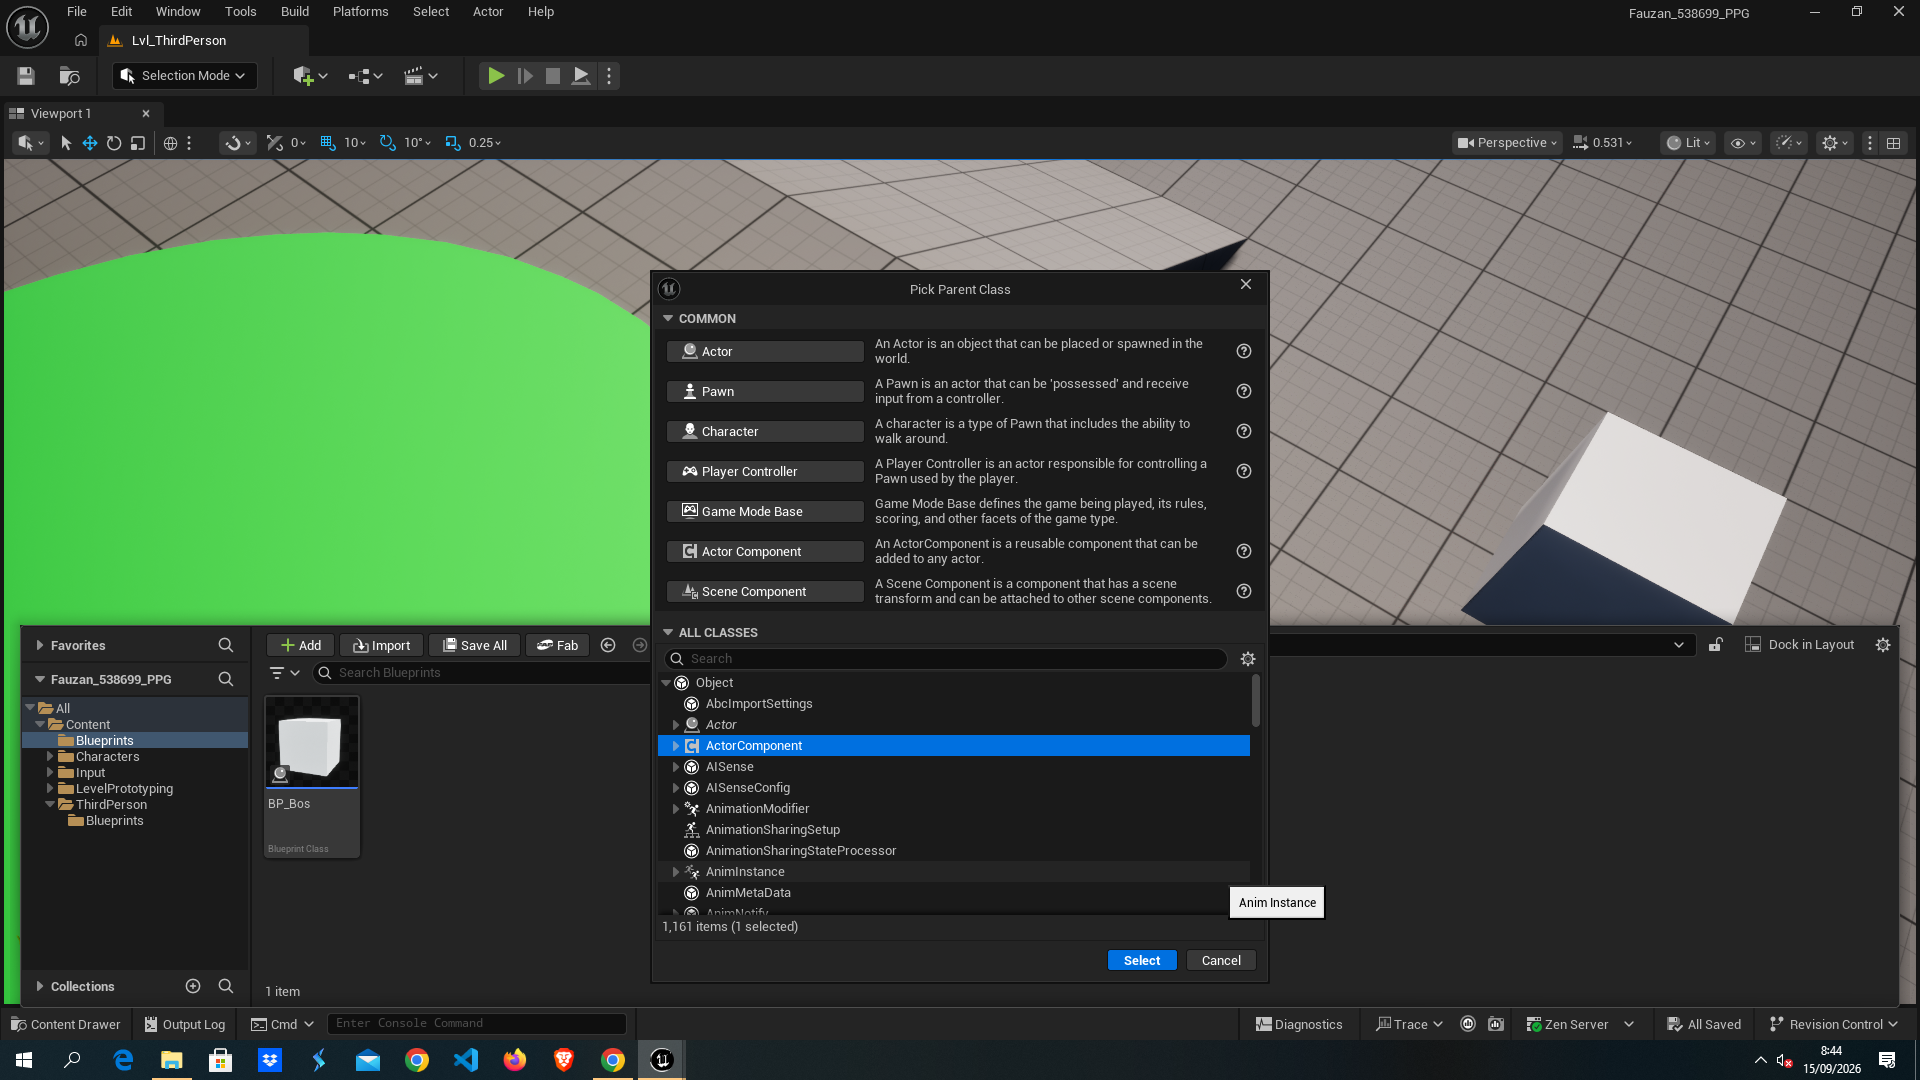
\includegraphics[width=0.8\textwidth]{resource/Dokumentasi/1.png}
  \caption{Pembuatan Blueprint Class bertipe Actor Component BPC\_Health}
  \label{fig:bpc-health-create}
\end{figure}

\par Berdasarkan Gambar \ref{fig:bpc-health-create}, langkah awal yang saya lakukan adalah membuat aset \textit{Blueprint Class} baru pada Content Drawer. Melalui menu klik kanan di area kerja direktori proyek atau menekan tombol \textit{+ Add}, saya memilih opsi \textit{Blueprint Class} yang memunculkan jendela dialog pemilihan kelas induk (\textit{Pick Parent Class}). Pada jendela ini, alih-alih memilih kelas \textit{Actor} biasa, saya memilih kelas \textit{Actor Component} sebagai basisnya. Aset yang baru terbentuk ini saya beri nama \texttt{BPC\_Health} dengan menggunakan prefiks standar \texttt{BPC\_} (\textit{Blueprint Component}) sesuai dengan konvensi penamaan resmi Unreal Engine untuk menandakan bahwa aset tersebut merupakan komponen logika modular yang dapat disematkan ke berbagai aktor di dalam permainan.

\begin{figure}[H]
  \centering
  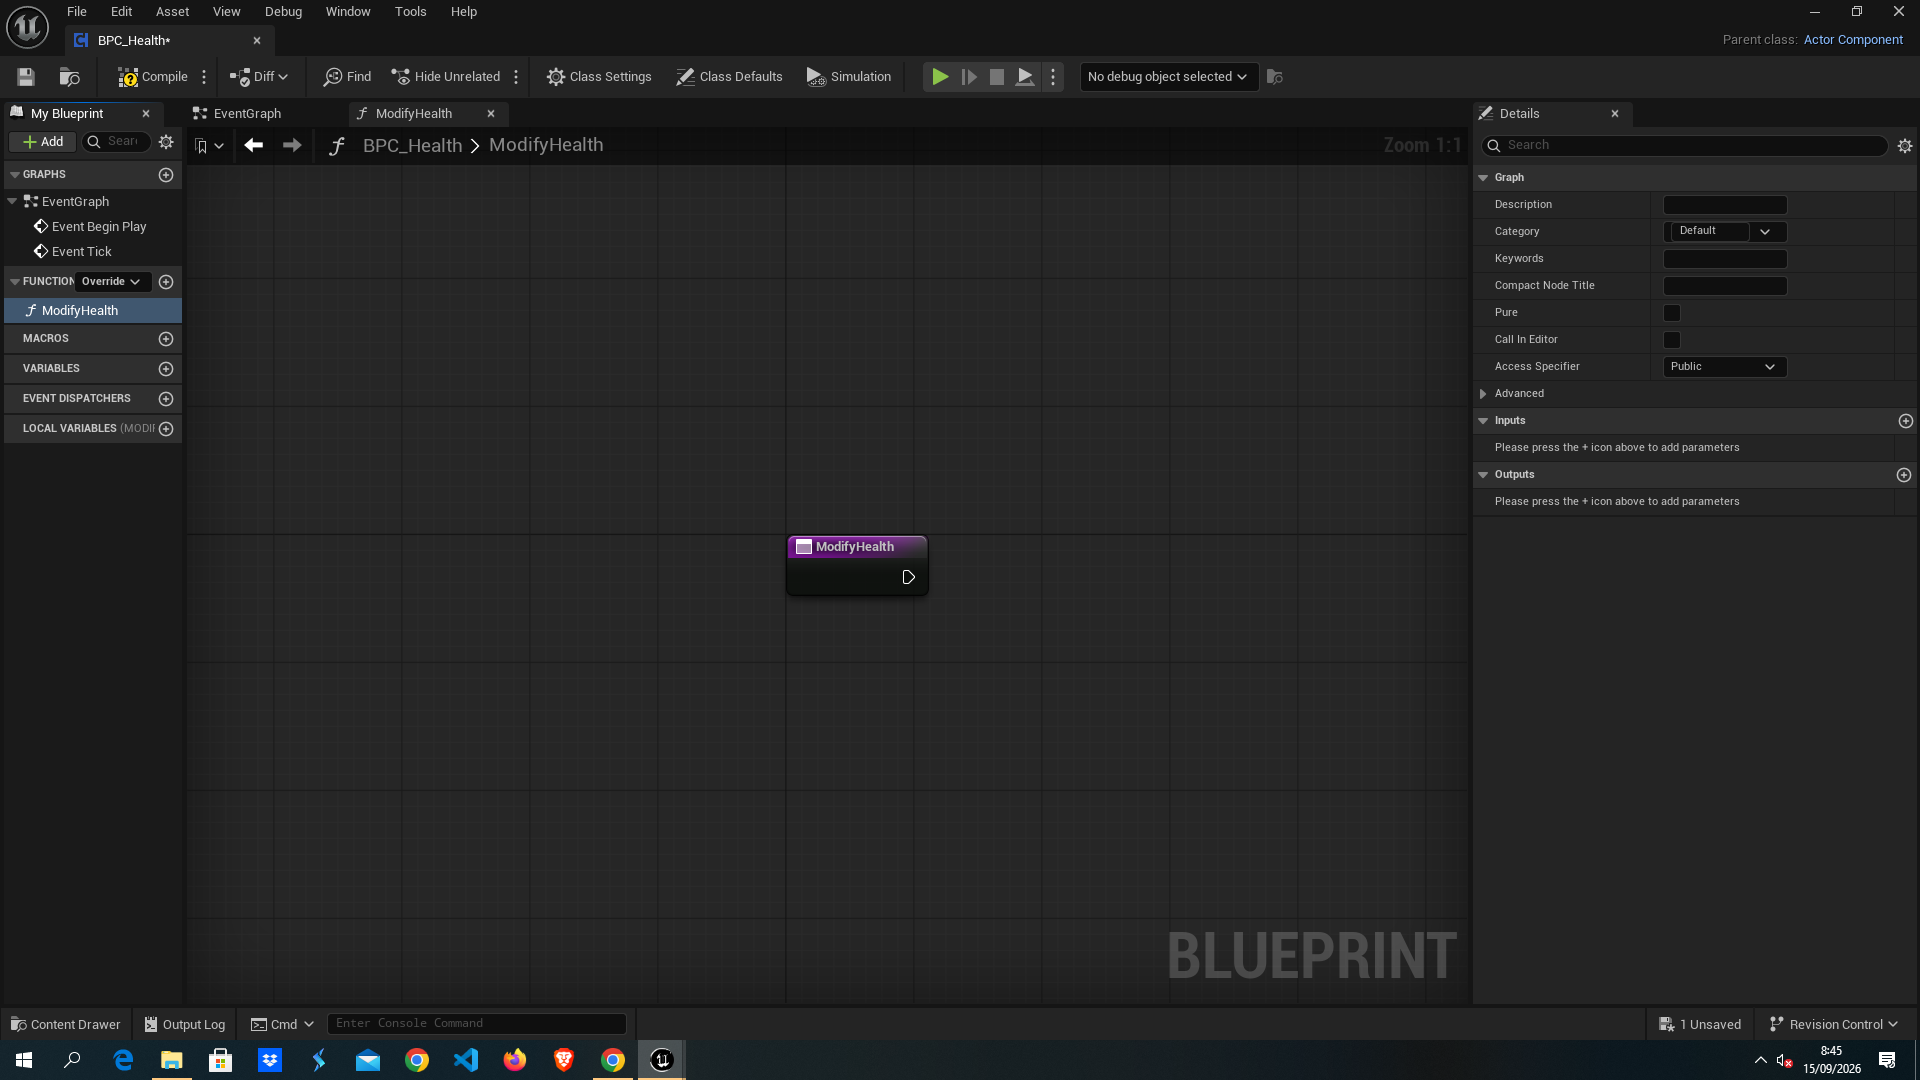
\includegraphics[width=0.8\textwidth]{resource/Dokumentasi/2.png}
  \caption{Deklarasi Variabel Health pada BPC\_Health}
  \label{fig:var-health}
\end{figure}

\par Setelah berkas \texttt{BPC\_Health} terbuka di editor, langkah selanjutnya adalah mendeklarasikan penampung data numerik status kesehatan sebagaimana diperlihatkan pada Gambar \ref{fig:var-health}. Pada panel \textit{My Blueprint} di sisi kiri, saya menuju ke bagian \textit{Variables} dan mengeklik tombol \textit{+ Add}. Variabel baru tersebut saya beri nama \texttt{Health} dan menyetel tipe datanya menjadi \textit{Float} (presisi tunggal) yang ditandai dengan kode warna hijau terang pada pin Unreal Engine. Nilai variabel ini berfungsi menyimpan jumlah darah aktual entitas saat permainan berjalan secara waktu nyata (\textit{runtime}). Setelah melakukan proses kompilasi awal, saya menetapkan nilai bawaannya (\textit{Default Value}) sebesar 100.0 pada panel \textit{Details} di sisi kanan editor.

\begin{figure}[H]
  \centering
  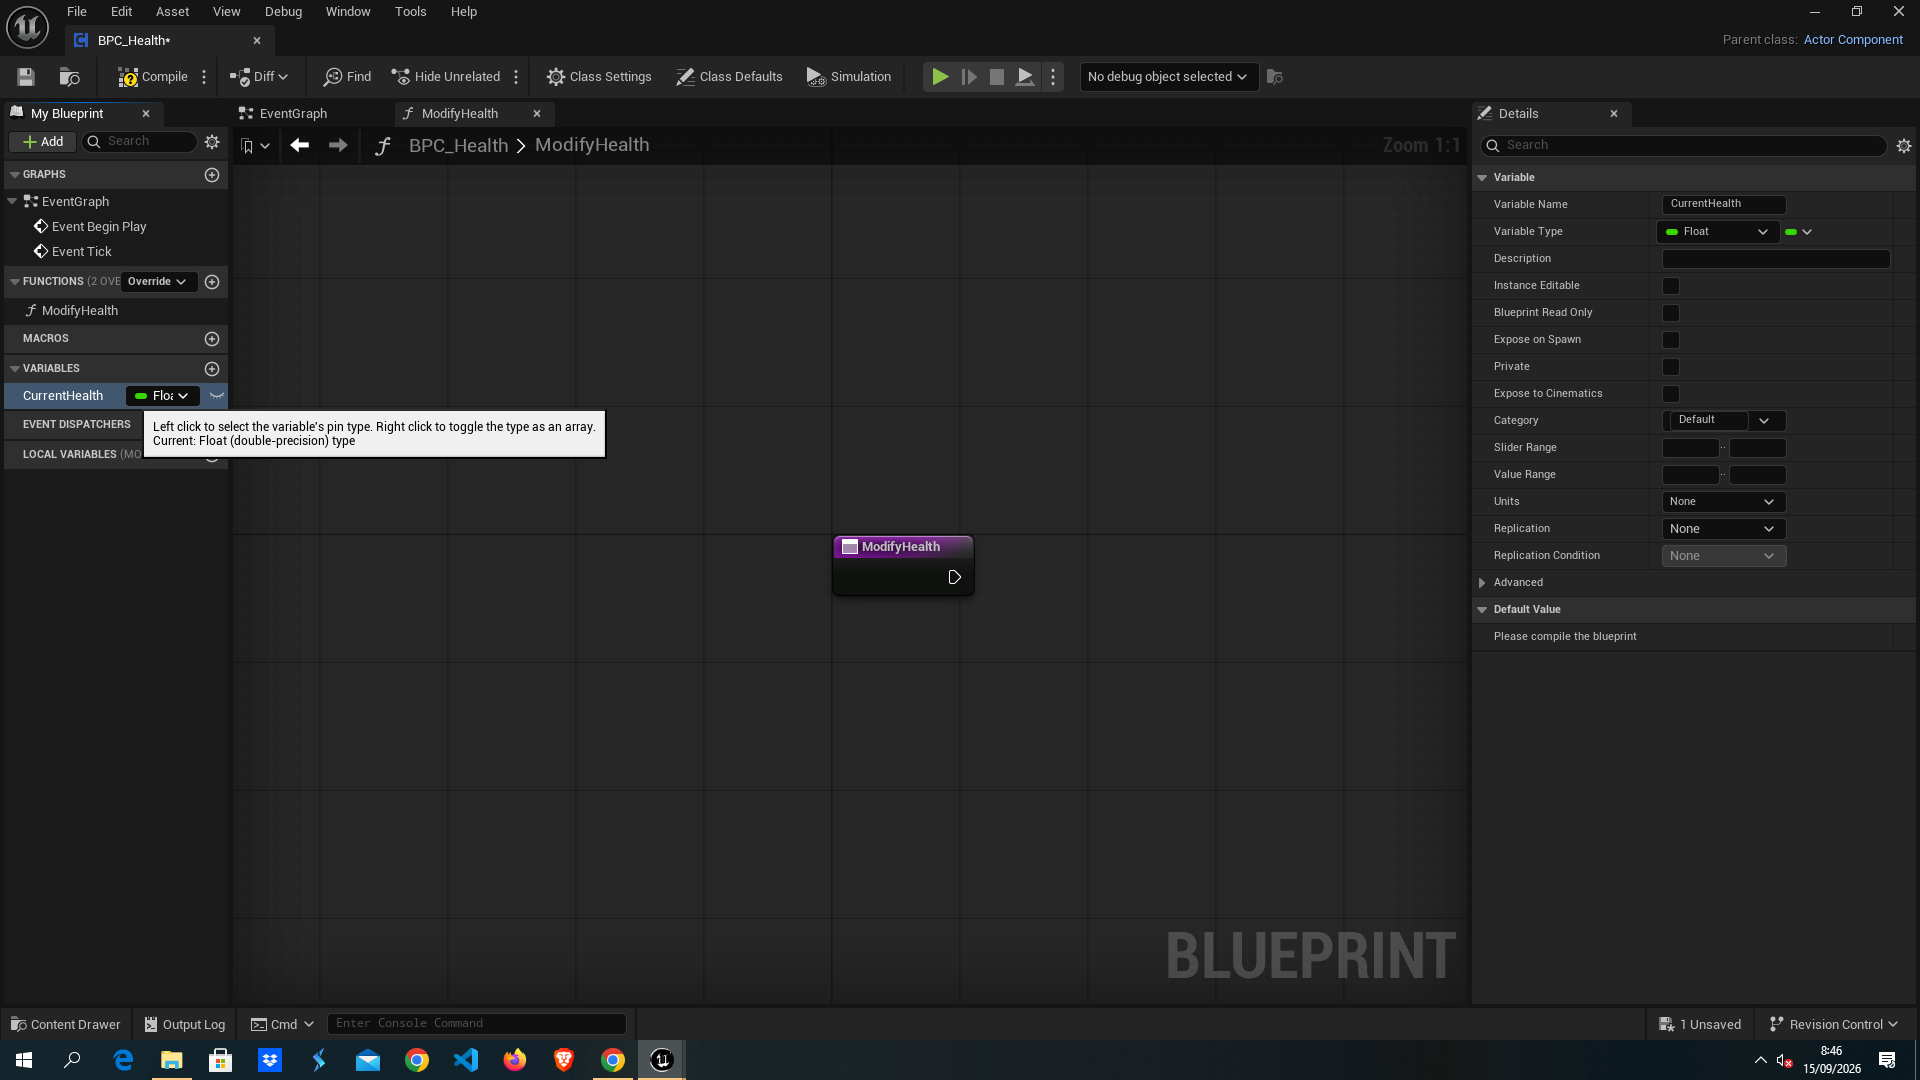
\includegraphics[width=0.8\textwidth]{resource/Dokumentasi/3.png}
  \caption{Deklarasi Variabel MaxHealth pada BPC\_Health}
  \label{fig:var-maxhealth}
\end{figure}

\par Melanjutkan pengelolaan atribut entitas, Gambar \ref{fig:var-maxhealth} memperlihatkan pembuatan variabel kedua yang saya namai \texttt{MaxHealth}. Variabel ini juga saya atur dengan tipe data \textit{Float} dan nilai bawaan sebesar 100.0 setelah proses kompilasi. Keberadaan variabel \texttt{MaxHealth} sangat esensial dalam arsitektur sistem permainan karena bertindak sebagai konstanta batas atas kapasitas maksimum kesehatan entitas. Nilai ini menjadi parameter acuan mutlak dalam operasi pembatasan matematis (\textit{clamping}) agar penambahan darah dari efek pemulihan tidak pernah melampaui kapasitas normal yang telah ditetapkan oleh desainer permainan.

\begin{figure}[H]
  \centering
  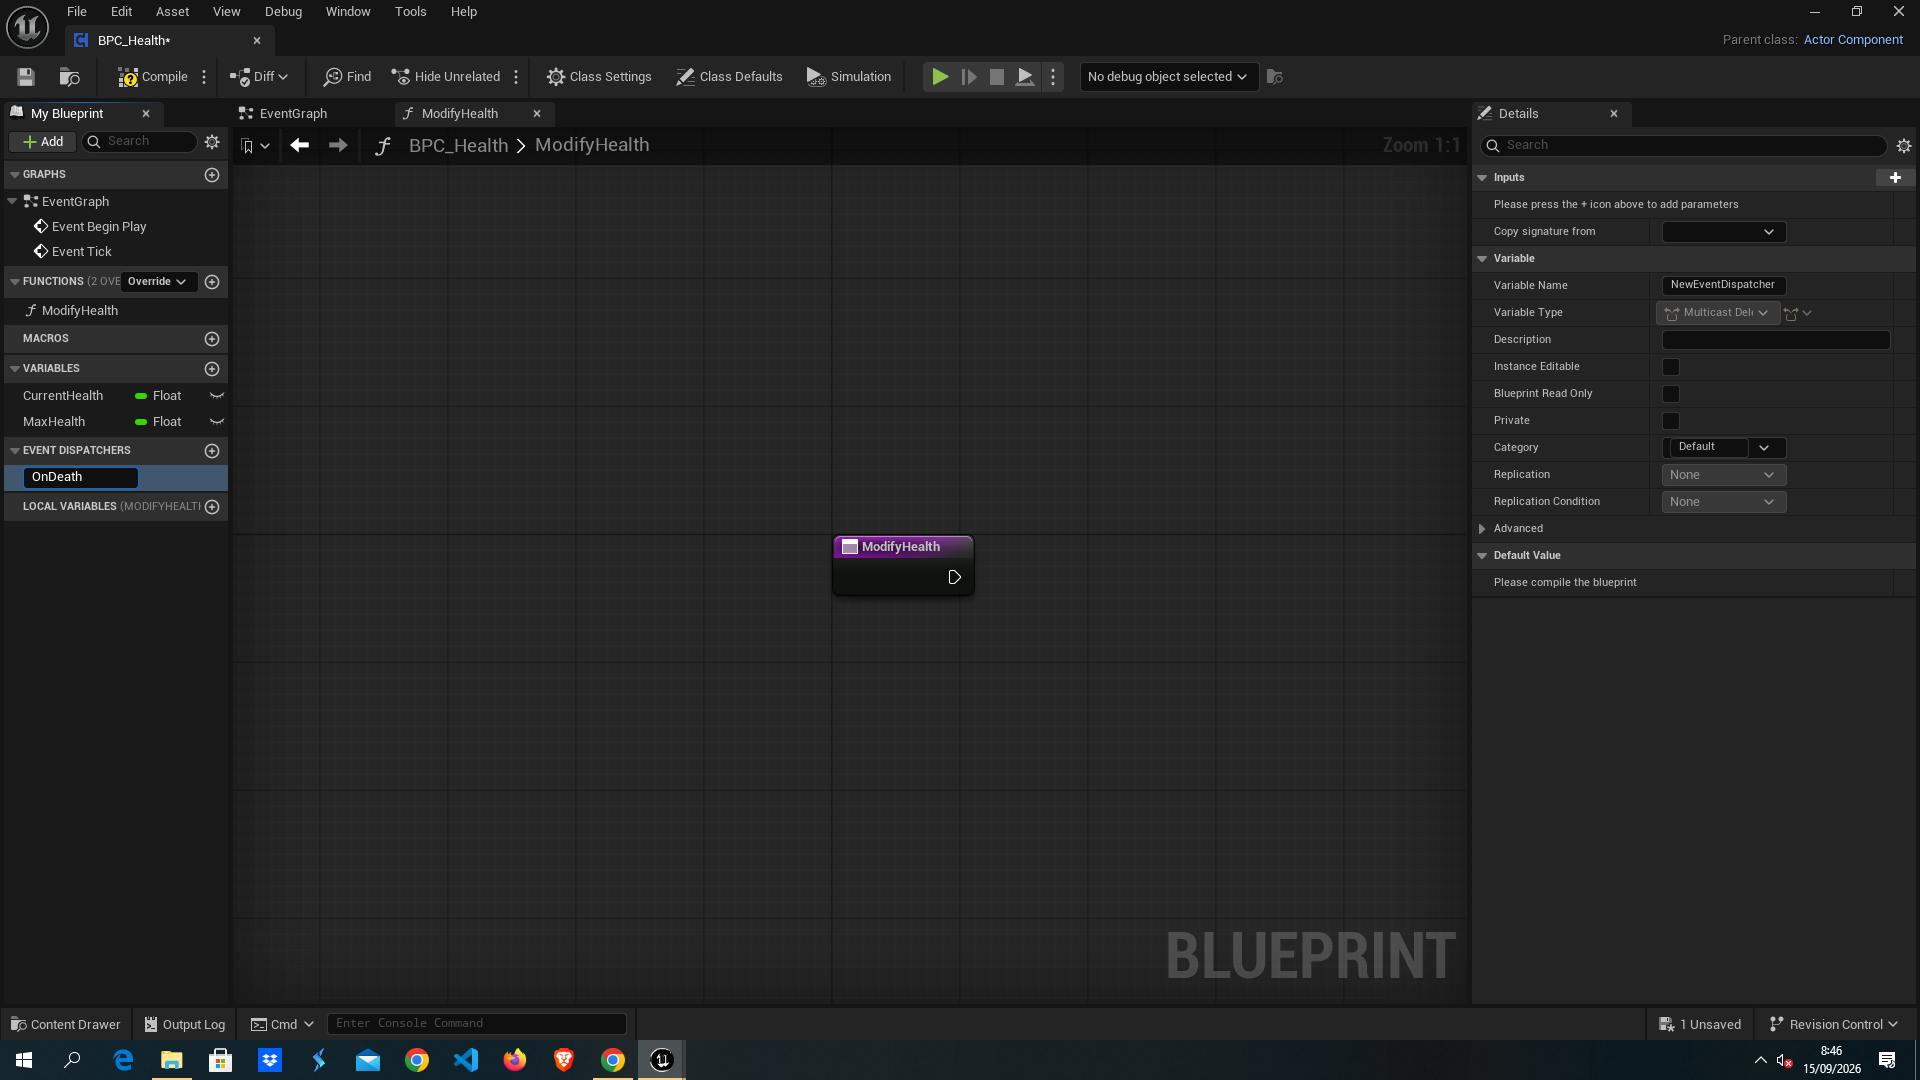
\includegraphics[width=0.8\textwidth]{resource/Dokumentasi/4.png}
  \caption{Pembuatan Event Dispatcher OnDeath}
  \label{fig:event-dispatcher-ondeath}
\end{figure}

\par Berdasarkan Gambar \ref{fig:event-dispatcher-ondeath}, saya kemudian merancang mekanisme komunikasi asinkron dengan membuat sebuah \textit{Event Dispatcher} baru bernama \texttt{OnDeath}. Pembuatan ini dilakukan melalui panel \textit{My Blueprint} pada kategori \textit{Event Dispatchers} dengan mengeklik tombol \textit{+ Add}. Pemanfaatan \textit{Event Dispatcher} bertujuan menerapkan paradigma arsitektur berbasis kejadian (\textit{event-driven architecture}), di mana komponen \texttt{BPC\_Health} dapat menyiarkan sinyal kematian secara independen tanpa perlu mengetahui secara langsung kelas aktor mana saja yang mendengarkannya, sehingga mencegah terjadinya keterikatan langsung (\textit{tight coupling}) maupun dependensi sirkular antar-kelas.

\begin{figure}[H]
  \centering
  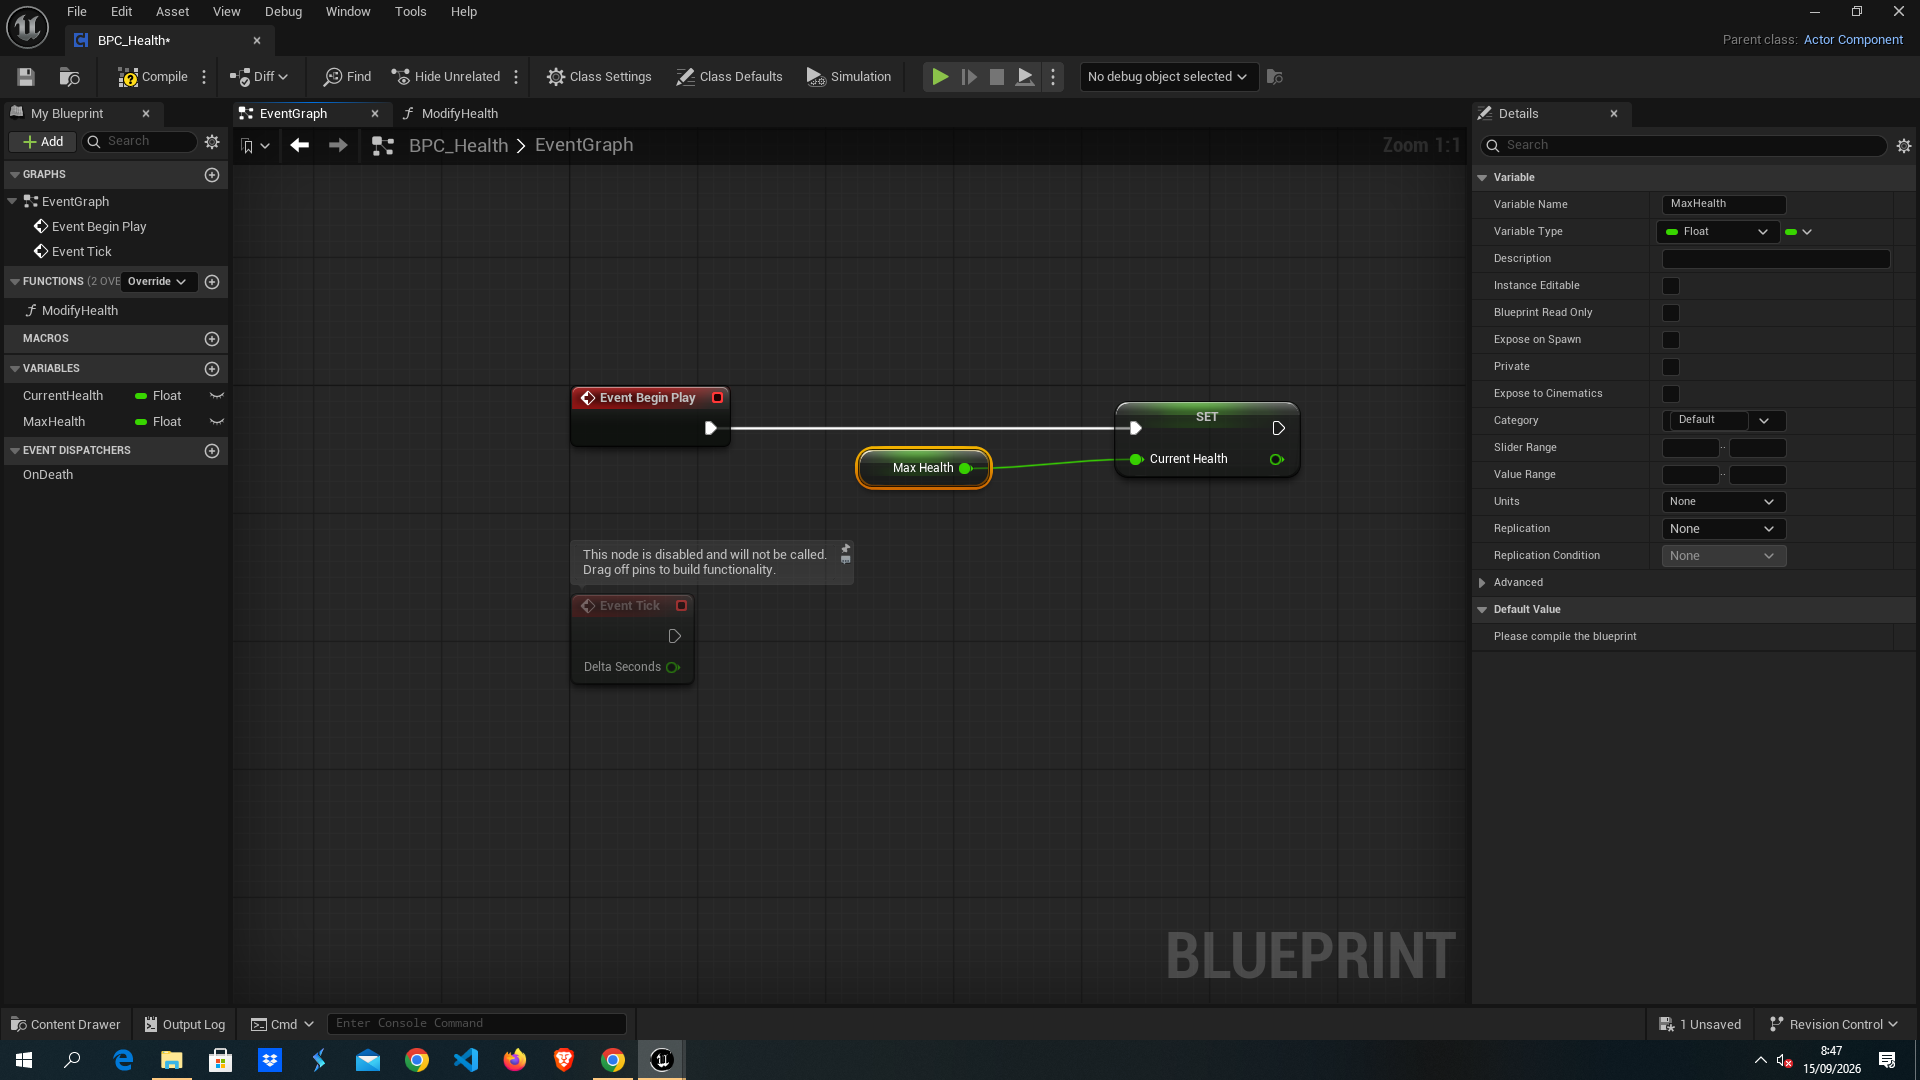
\includegraphics[width=0.8\textwidth]{resource/Dokumentasi/5.png}
  \caption{Pembuatan Fungsi Kustom ModifyHealth}
  \label{fig:func-modifyhealth}
\end{figure}

\par Langkah berikutnya yang saya laksanakan adalah merancang fungsi pengendali nilai kesehatan, seperti tampak pada Gambar \ref{fig:func-modifyhealth}. Pada panel \textit{My Blueprint} kategori \textit{Functions}, saya menambahkan sebuah fungsi kustom baru yang diberi nama \texttt{ModifyHealth}. Melalui panel \textit{Details} fungsi tersebut, saya menambahkan parameter masukan (\textit{Inputs}) bertipe data \textit{Float} dengan nama \texttt{Amount}. Fungsi ini dirancang sebagai satu-satunya gerbang enkapsulasi untuk memanipulasi status kesehatan entitas, di mana nilai masukan positif akan merepresentasikan pemulihan darah (\textit{healing}), sedangkan nilai negatif akan merepresentasikan pengurangan darah akibat serangan atau kerusakan (\textit{damage}).

\begin{figure}[H]
  \centering
  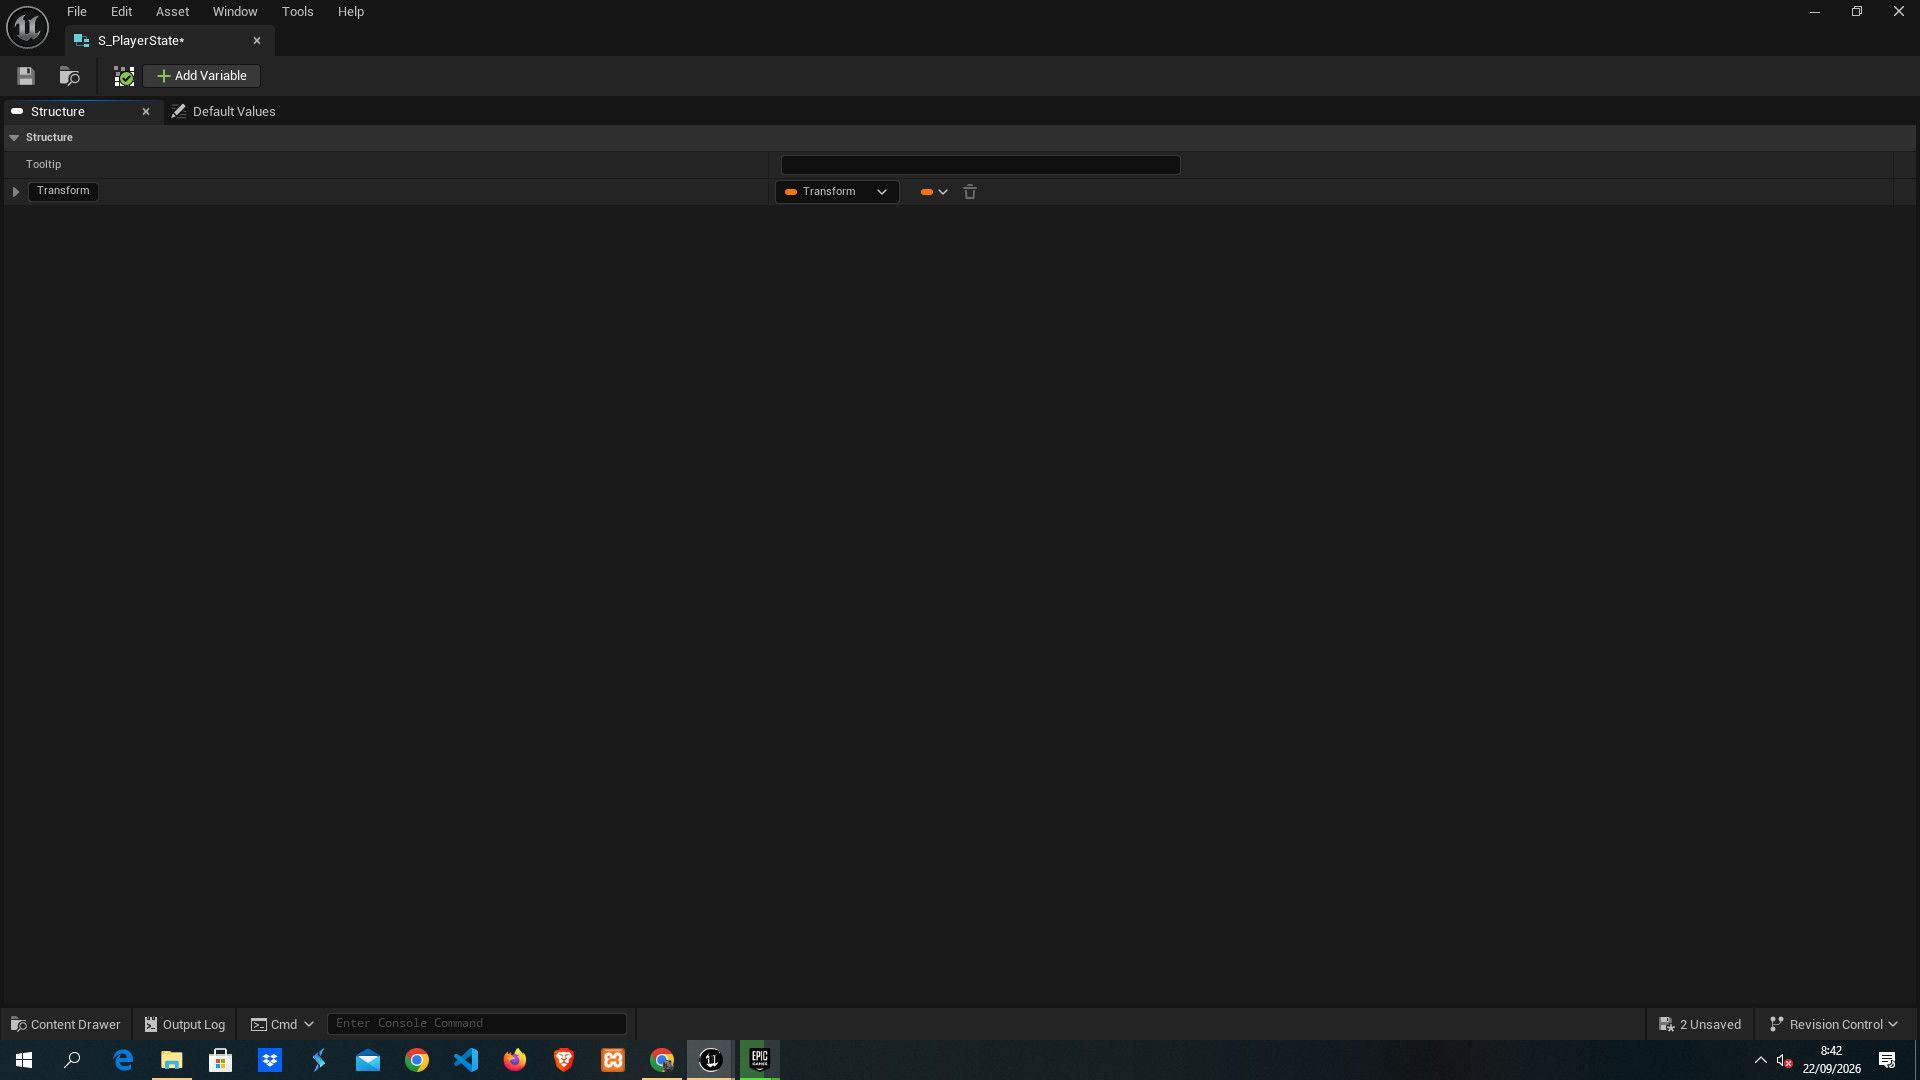
\includegraphics[width=0.8\textwidth]{resource/Dokumentasi/6.png}
  \caption{Implementasi Logika Kalkulasi dan Clamping pada ModifyHealth}
  \label{fig:modifyhealth-clamping}
\end{figure}

\par Pada Gambar \ref{fig:modifyhealth-clamping}, saya menyusun alur logika matematika visual di dalam lembar kerja fungsi \texttt{ModifyHealth}. Saya mengambil nilai variabel \texttt{Health} saat ini melalui node \textit{getter} dan menjumlahkannya dengan parameter masukan \texttt{Amount} menggunakan operator penambahan (\textit{Add Float + Float}). Untuk mencegah terjadinya anomali nilai, hasil penjumlahan tersebut dialirkan menuju pin masukan node \texttt{Clamp (Float)}. Saya menyetel batas minimum (\textit{Min}) pada nilai 0.0 dan menghubungkan batas maksimum (\textit{Max}) ke variabel \textit{getter} \texttt{MaxHealth}. Keluaran dari node pembatas ini kemudian disimpan kembali ke dalam variabel \texttt{Health} melalui node \textit{setter}, menjamin bahwa nilai kesehatan akan selalu berada dalam rentang valid antara 0.0 hingga 100.0.

\begin{figure}[H]
  \centering
  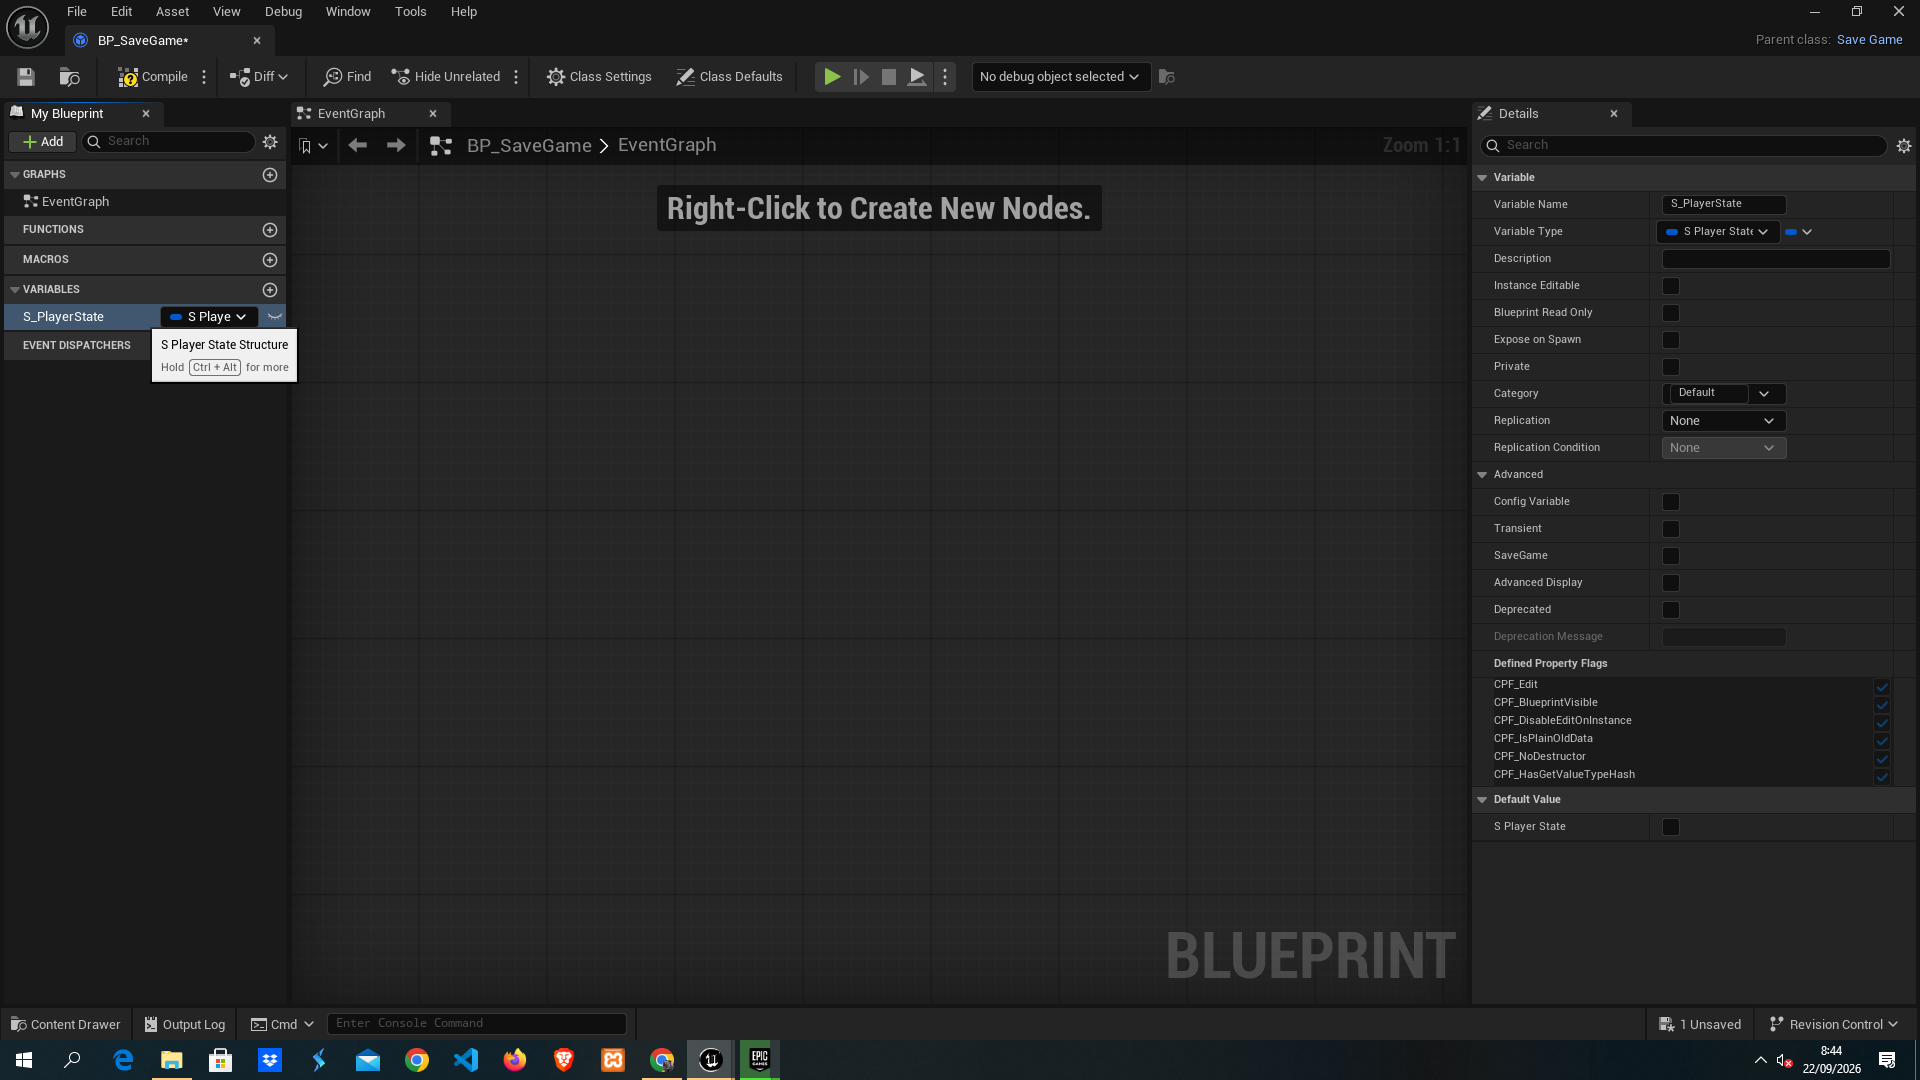
\includegraphics[width=0.8\textwidth]{resource/Dokumentasi/7.png}
  \caption{Pengecekan Kondisi Kematian dan Pemanggilan OnDeath}
  \label{fig:modifyhealth-branch-ondeath}
\end{figure}

\par Melengkapi logika fungsi \texttt{ModifyHealth}, Gambar \ref{fig:modifyhealth-branch-ondeath} memperlihatkan penambahan evaluasi kondisi untuk mendeteksi kematian entitas. Tepat setelah node \textit{setter} \texttt{Health}, saya menambahkan node percabangan \texttt{Branch}. Pin kondisi (\textit{Condition}) dihubungkan dengan operator pembanding \texttt{Less Equal (Float <= Float)} yang mengevaluasi apakah nilai \texttt{Health} telah bernilai kurang dari atau sama dengan 0.0. Apabila kondisi tersebut terpenuhi (\textit{True}), alur eksekusi langsung memicu node \texttt{Call OnDeath}. Tindakan ini memancarkan sinyal delegasi bahwa entitas telah kehabisan darah kepada seluruh sistem atau aktor yang telah mendaftarkan diri sebagai pendengar (\textit{listener}).

\subsection{Integrasi Actor Component dan Penanganan Event Kematian Karakter}

\par Setelah logika modular pada komponen kesehatan \texttt{BPC\_Health} selesai dibangun dan dikompilasi secara sempurna, tahapan berikutnya adalah mengintegrasikan komponen tersebut ke dalam kelas karakter pemain utama (\texttt{BP\_ThirdPersonCharacter}) serta menyusun skema respons visual saat karakter mengalami peristiwa kematian.

\begin{figure}[H]
  \centering
  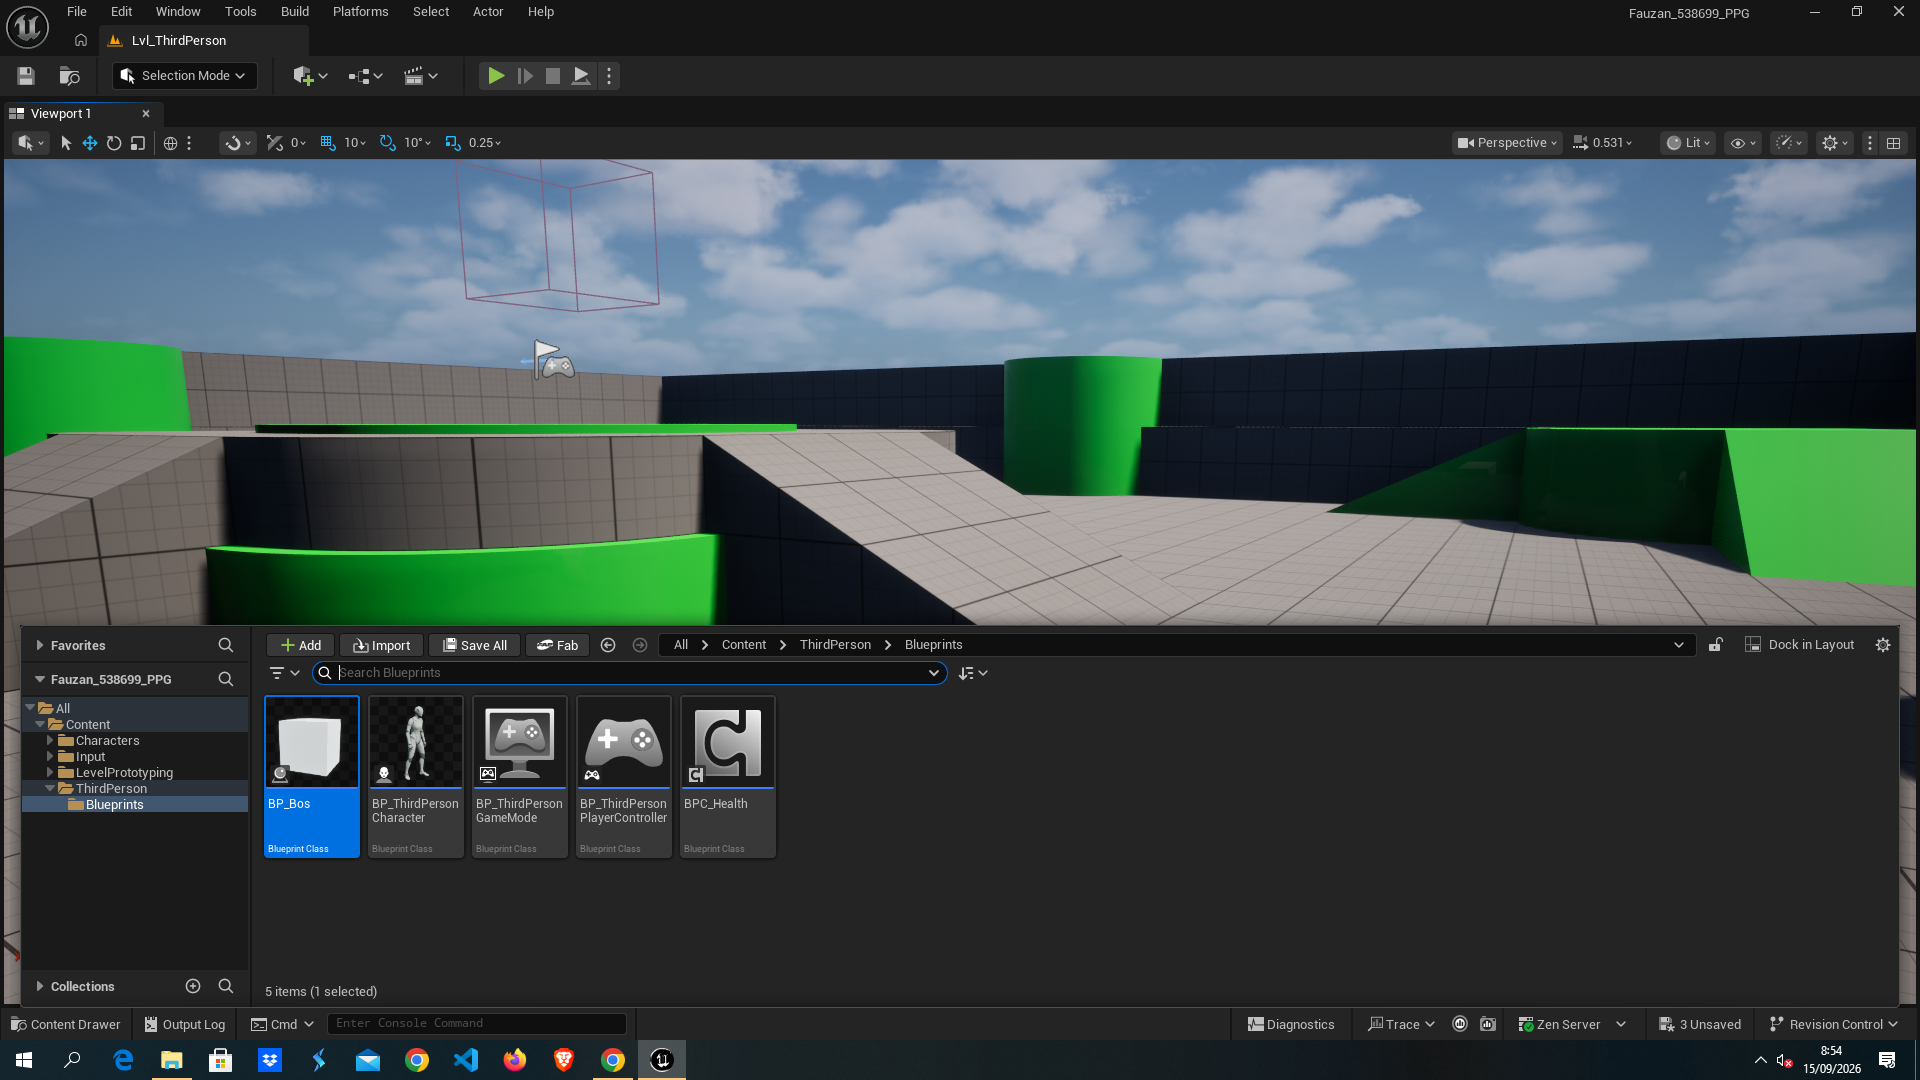
\includegraphics[width=0.8\textwidth]{resource/Dokumentasi/8.png}
  \caption{Membuka Event Graph BP\_ThirdPersonCharacter}
  \label{fig:open-thirdpersoncharacter}
\end{figure}

\par Berdasarkan Gambar \ref{fig:open-thirdpersoncharacter}, saya membuka aset karakter \texttt{BP\_ThirdPersonCharacter} di dalam folder ThirdPerson. Setelah jendela editor terbuka, saya beralih ke tab \textit{Event Graph} untuk memeriksa lembar kerja logika serta mempersiapkan penyematan komponen kesehatan yang telah dibuat.

\begin{figure}[H]
  \centering
  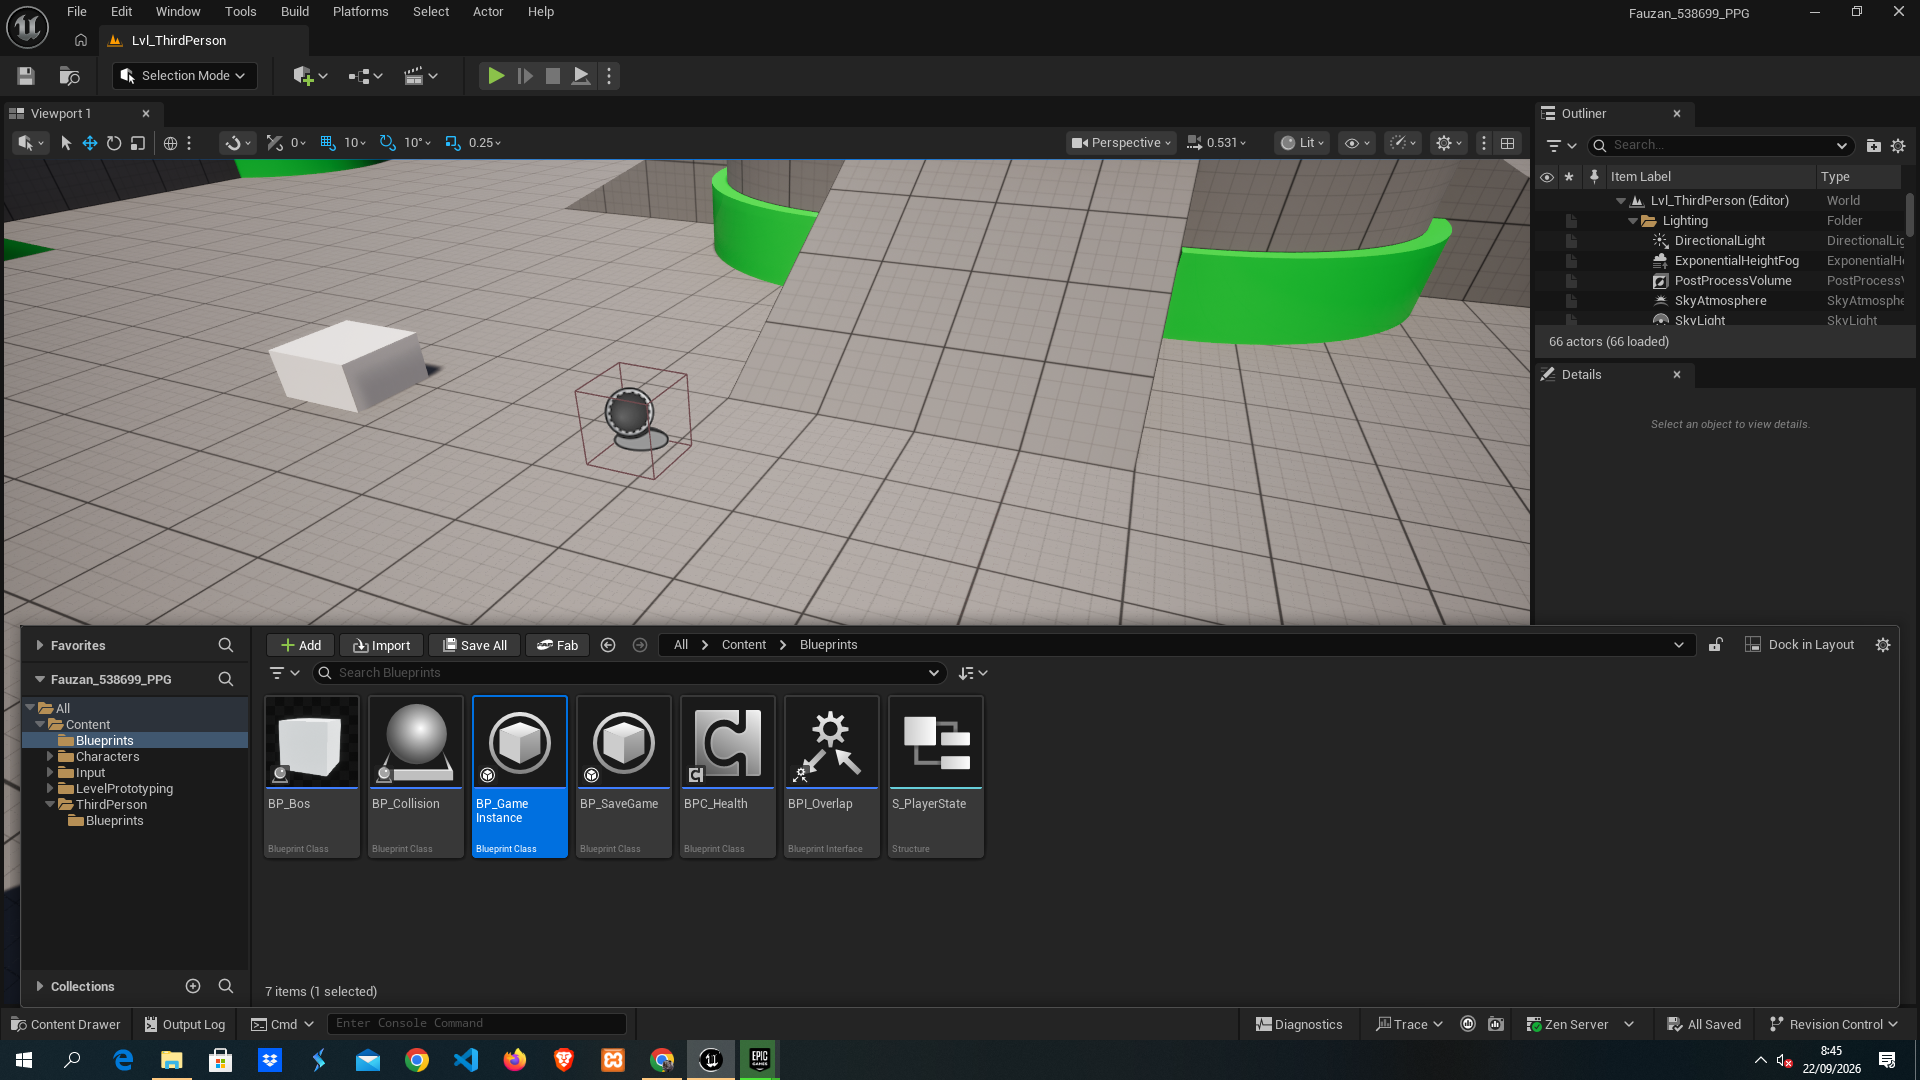
\includegraphics[width=0.8\textwidth]{resource/Dokumentasi/9.png}
  \caption{Penyematan Komponen BPC\_Health ke BP\_ThirdPersonCharacter}
  \label{fig:add-bpc-health-component}
\end{figure}

\par Pada Gambar \ref{fig:add-bpc-health-component}, saya menyematkan komponen \texttt{BPC\_Health} ke dalam hierarki karakter pemain. Pada panel \textit{Components} yang terletak di pojok kiri atas jendela editor, saya mengeklik tombol \textit{+ Add}, mengetikkan kata kunci \texttt{BPC\_Health} pada bilah pencarian, dan memilih komponen tersebut. Melalui prinsip komposisi (\textit{composition over inheritance}), karakter pemain kini secara instan memiliki seluruh kapabilitas pengelolaan kesehatan, variabel status, fungsi perhitungan, dan pemancar sinyal kematian tanpa perlu menulis ulang logika tersebut di dalam grafik karakter.

\begin{figure}[H]
  \centering
  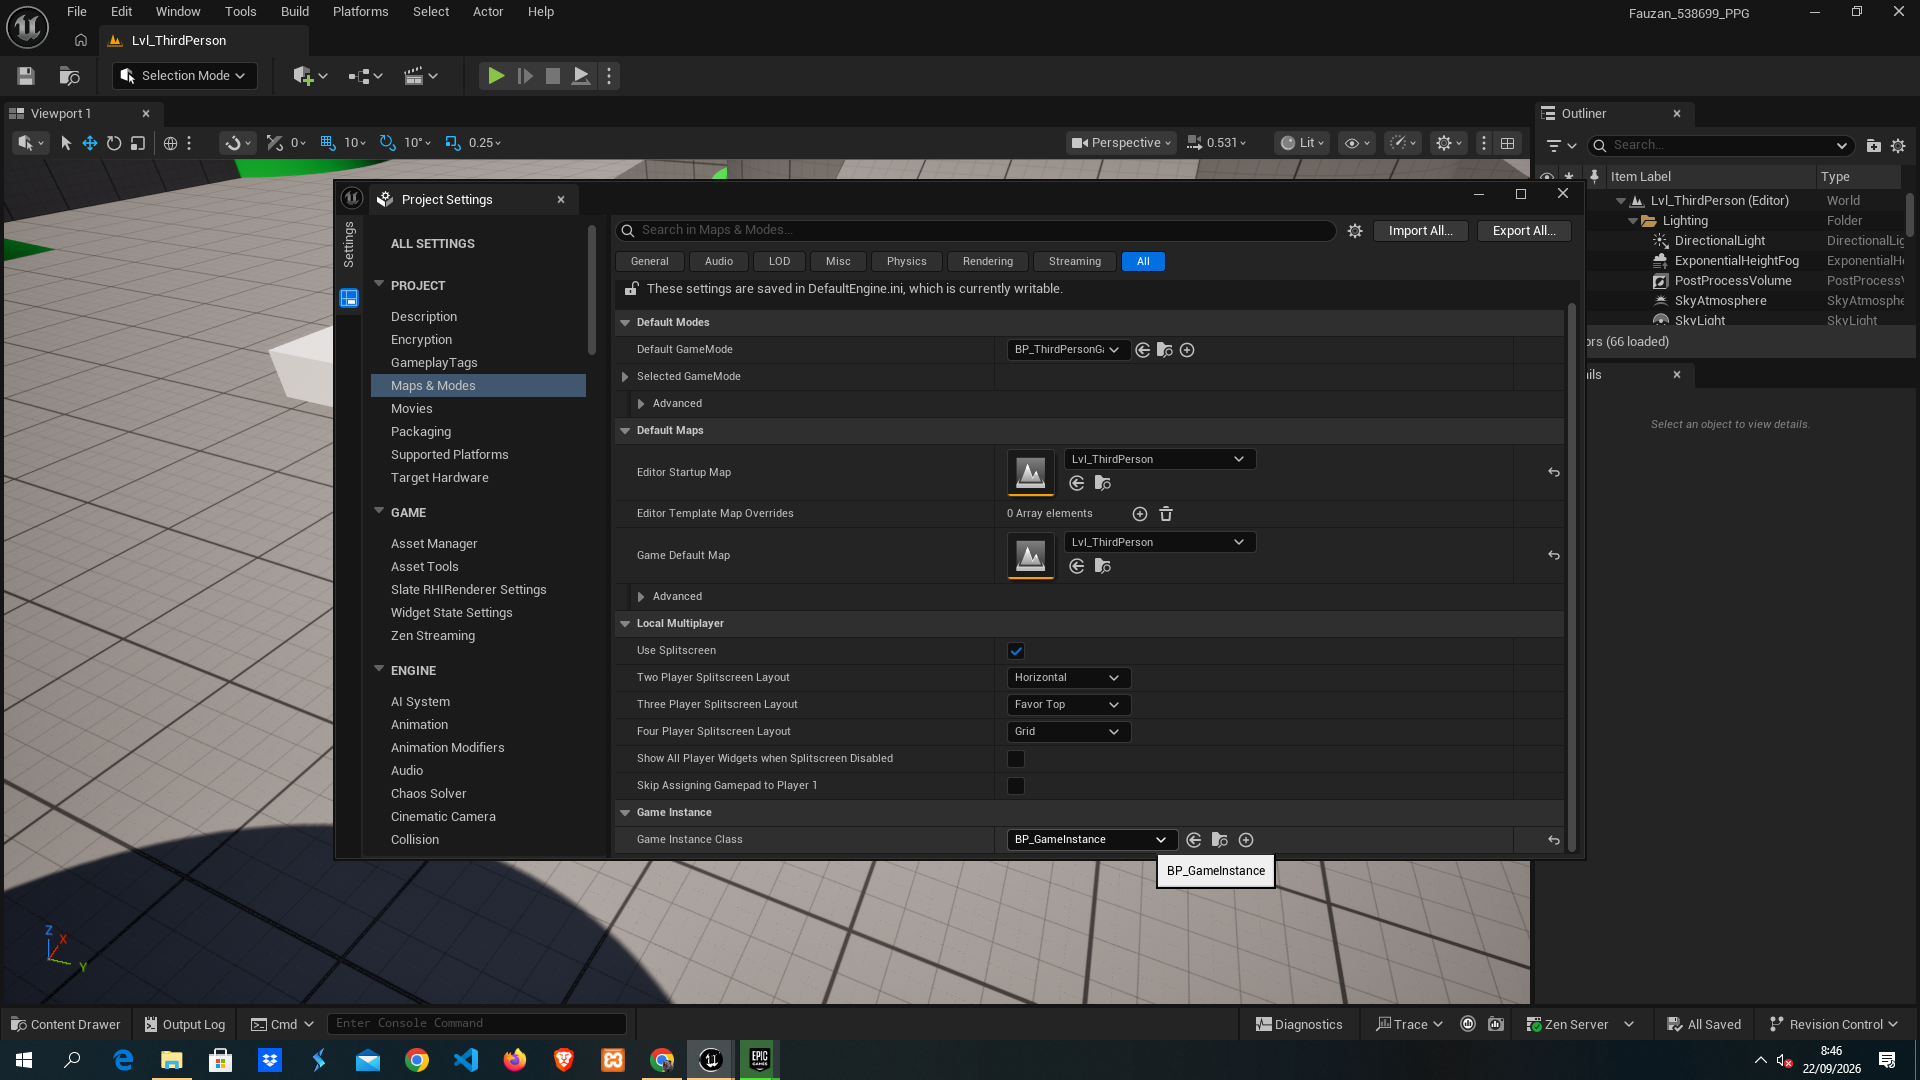
\includegraphics[width=0.8\textwidth]{resource/Dokumentasi/10.png}
  \caption{Pemanggilan Node Assign On Death pada BPC\_Health}
  \label{fig:assign-ondeath}
\end{figure}

\par Langkah berlanjut dengan mengonfigurasi penanganan sinyal kematian, seperti diperlihatkan pada Gambar \ref{fig:assign-ondeath}. Saya menyeret referensi komponen \texttt{BPC\_Health} dari panel \textit{Components} ke atas kanvas kerja \textit{Event Graph}. Dari pin keluaran referensi komponen tersebut, saya menarik kabel eksekusi dan mencari instruksi \texttt{Assign On Death}. Tindakan ini secara otomatis mengenerasikan dua buah node yang saling terhubung: sebuah node fungsi \texttt{Bind Event to OnDeath} dan sebuah node \textit{Custom Event} baru yang langsung tersambung ke pin delegasi \textit{Event}.

\begin{figure}[H]
  \centering
  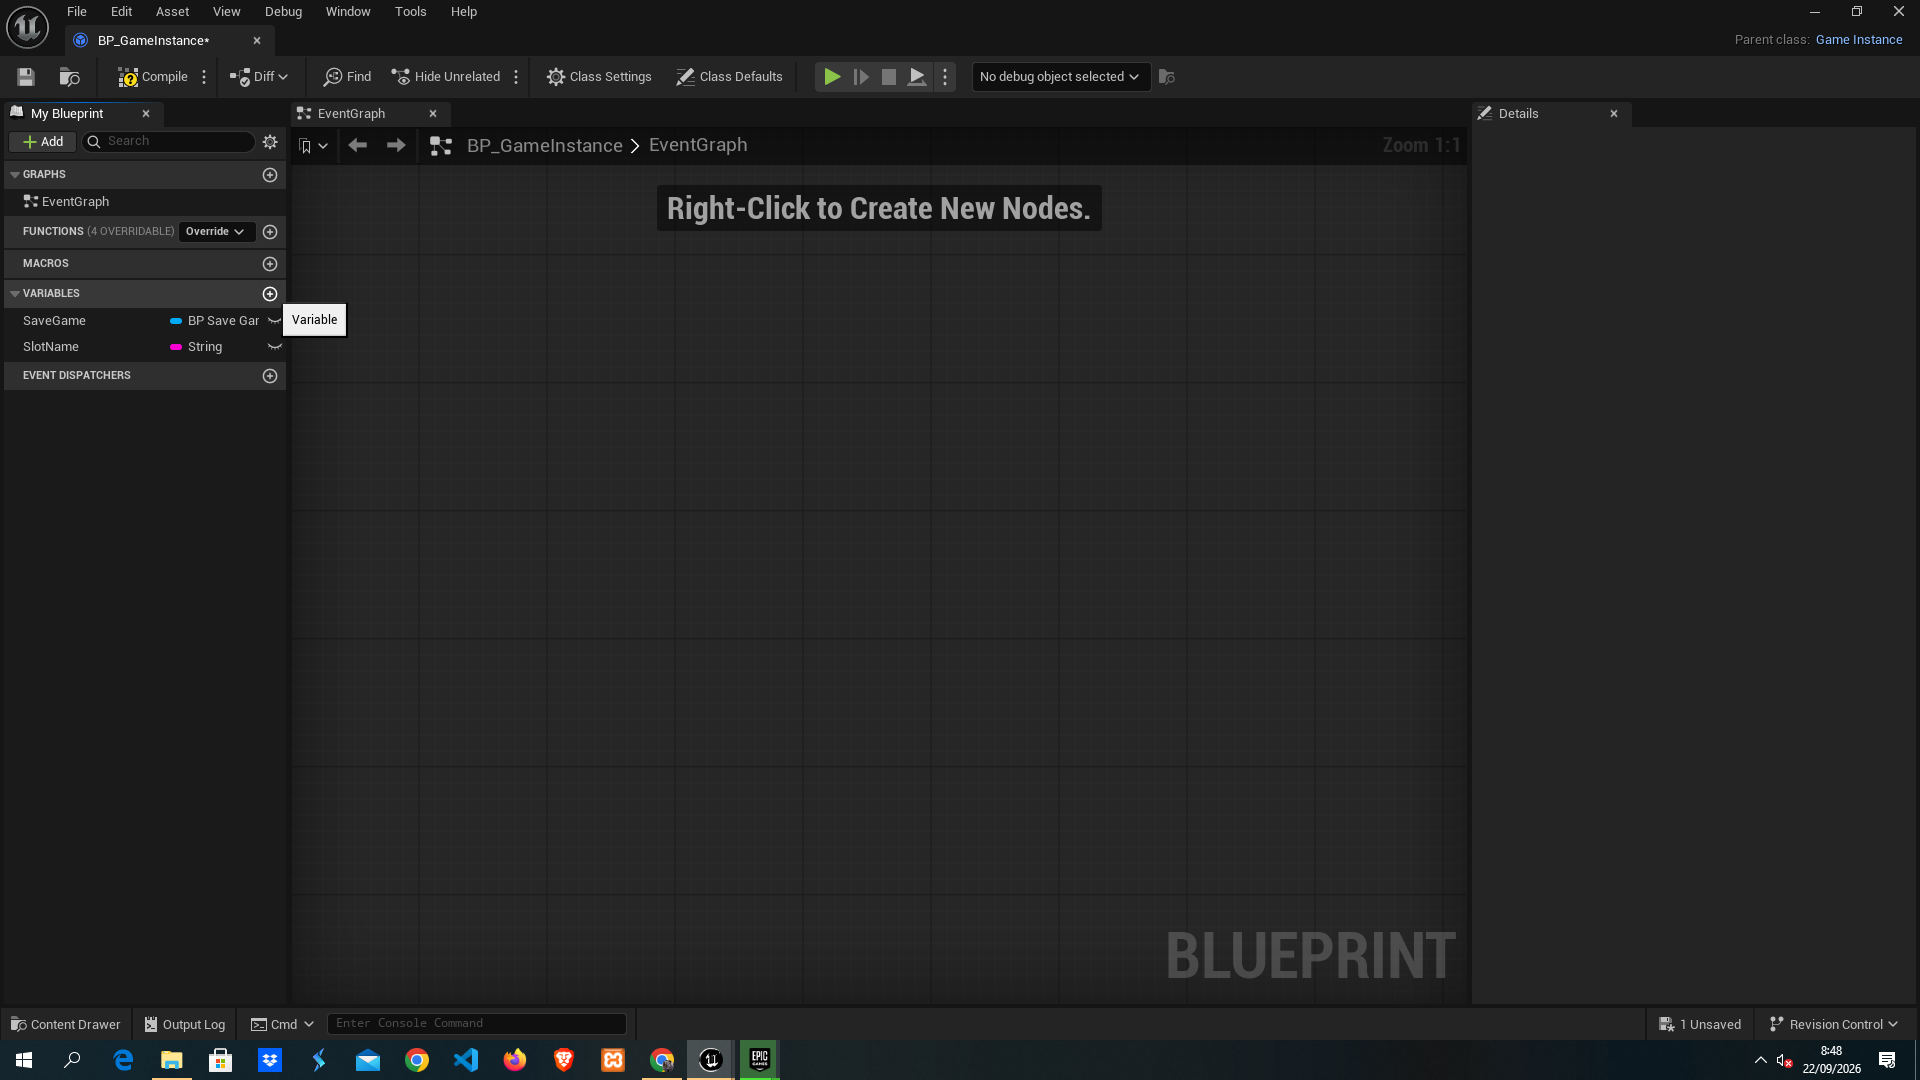
\includegraphics[width=0.8\textwidth]{resource/Dokumentasi/11.png}
  \caption{Menghubungkan Event BeginPlay ke Bind Event to OnDeath}
  \label{fig:bind-beginplay}
\end{figure}

\par Berdasarkan Gambar \ref{fig:bind-beginplay}, saya menyambungkan pin eksekusi dari node bawaan \textit{Event BeginPlay} milik \texttt{BP\_ThirdPersonCharacter} menuju ke pin eksekusi masukan pada node \texttt{Bind Event to OnDeath}. Konfigurasi ini menjamin bahwa sesaat setelah karakter diinisialisasi ke dalam dunia permainan saat awal sesi dijalankan, sistem karakter telah secara aktif mengikat dan mendaftarkan diri sebagai pendengar resmi terhadap sinyal kejadian kematian yang dipancarkan oleh komponen \texttt{BPC\_Health}.

\begin{figure}[H]
  \centering
  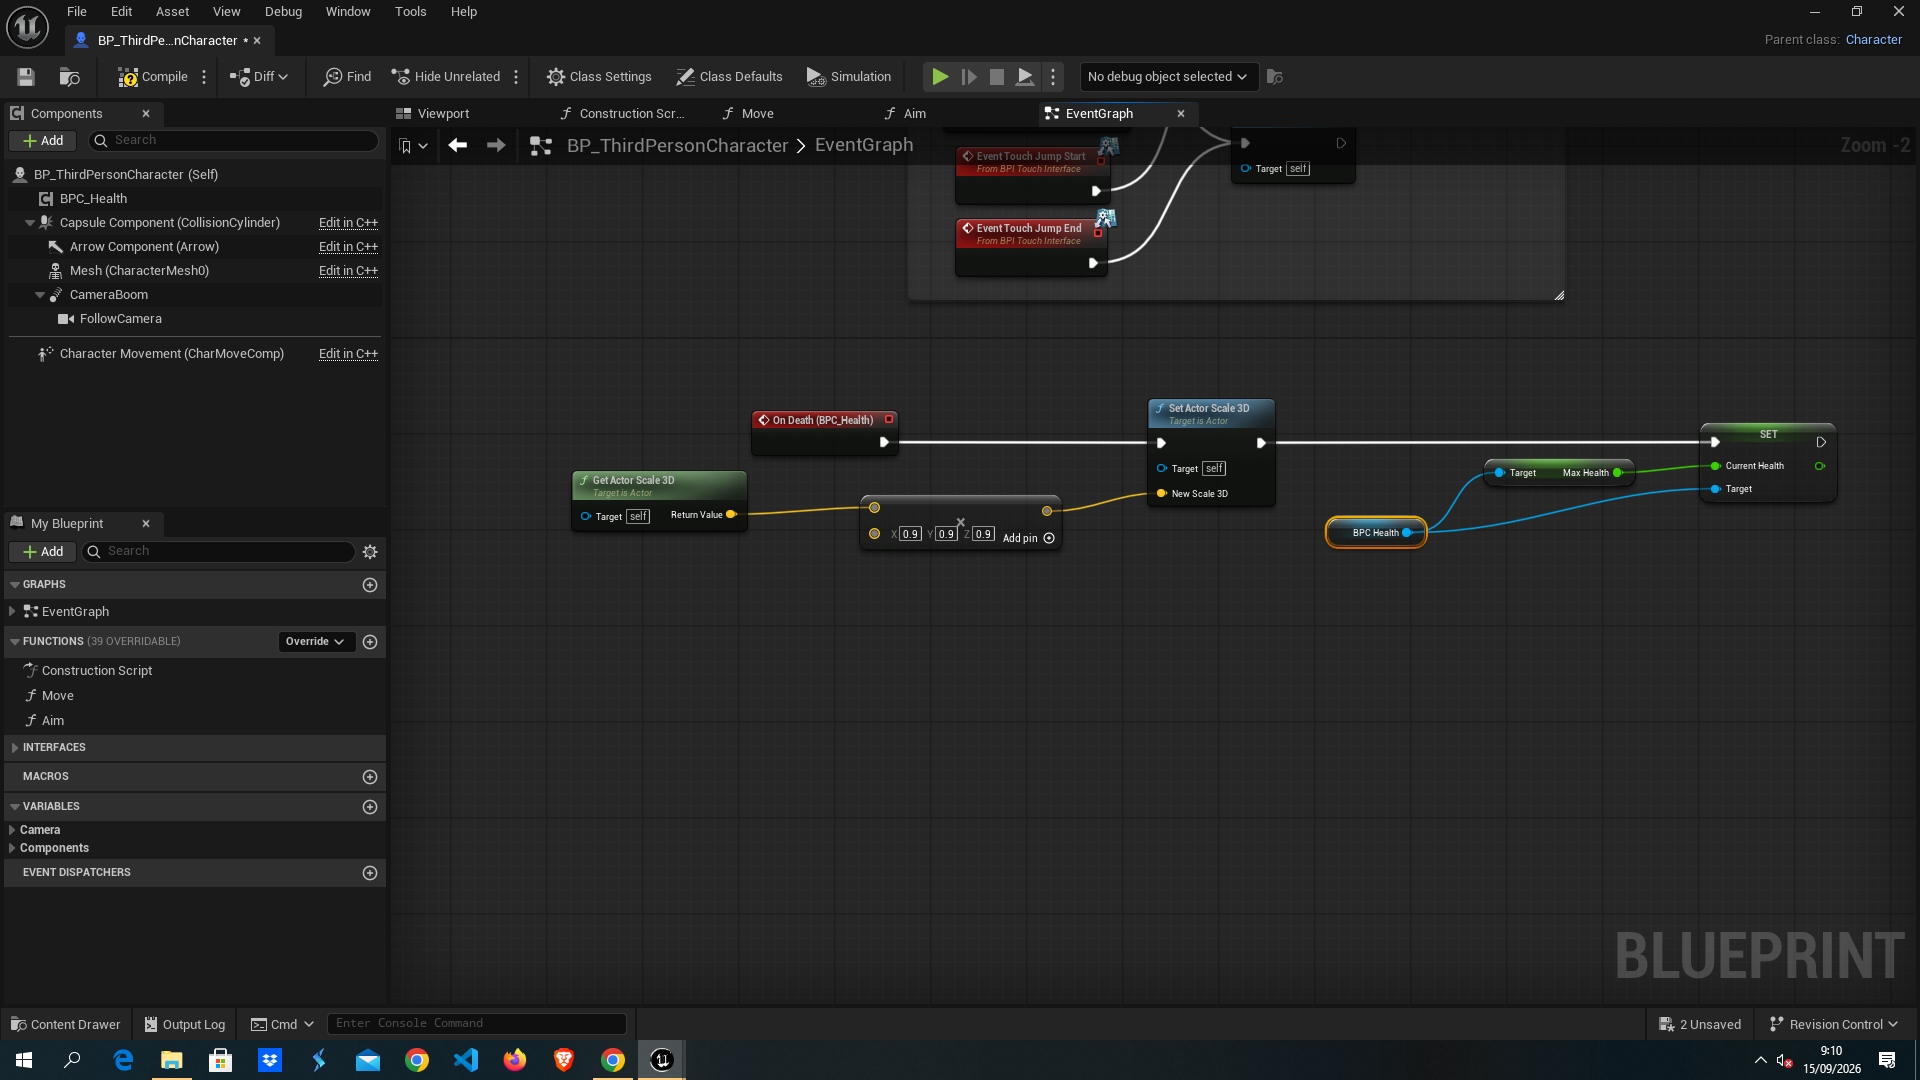
\includegraphics[width=0.8\textwidth]{resource/Dokumentasi/12.png}
  \caption{Implementasi Set Actor Scale 3D pada Event Respons OnDeath}
  \label{fig:set-actor-scale-death}
\end{figure}

\par Pada Gambar \ref{fig:set-actor-scale-death}, saya menyusun respons visual terhadap kematian karakter pada alur \textit{Custom Event} yang terikat dengan \texttt{OnDeath}. Dari pin eksekusi \textit{Custom Event} tersebut, saya memanggil node transformasi spasial \texttt{Set Actor Scale 3D}. Pin \textit{Target} dibiarkan merujuk ke \texttt{self} (aktor karakter itu sendiri), dan nilai pada parameter masukan \texttt{New Scale 3D} diatur menjadi nilai konstan 0.9 pada sumbu X, Y, dan Z. Melalui implementasi ini, saat karakter kehabisan darah dan sinyal kematian dipancarkan, ukuran tubuh karakter akan menyusut secara instan menjadi 90 persen dari ukuran aslinya sebagai umpan balik visual (\textit{visual feedback}) yang jelas bagi pemain bahwa karakter telah gugur.

\subsection{Pembuatan dan Implementasi Blueprint Interface (BPI\_Overlap)}

\par Untuk menghubungkan interaksi antara objek perintang di dalam dunia permainan dengan karakter pemain secara efisien, saya mengimplementasikan antarmuka \textit{Blueprint Interface}. Penggunaan antarmuka ini bertujuan mewujudkan komunikasi terkopel rendah (\textit{loosely coupled}), sehingga objek pemicu tabrakan dapat mengirimkan instruksi pengurangan darah ke sembarang aktor tanpa perlu melakukan operasi pengecekan tipe kelas secara langsung (\textit{hard casting}).

\begin{figure}[H]
  \centering
  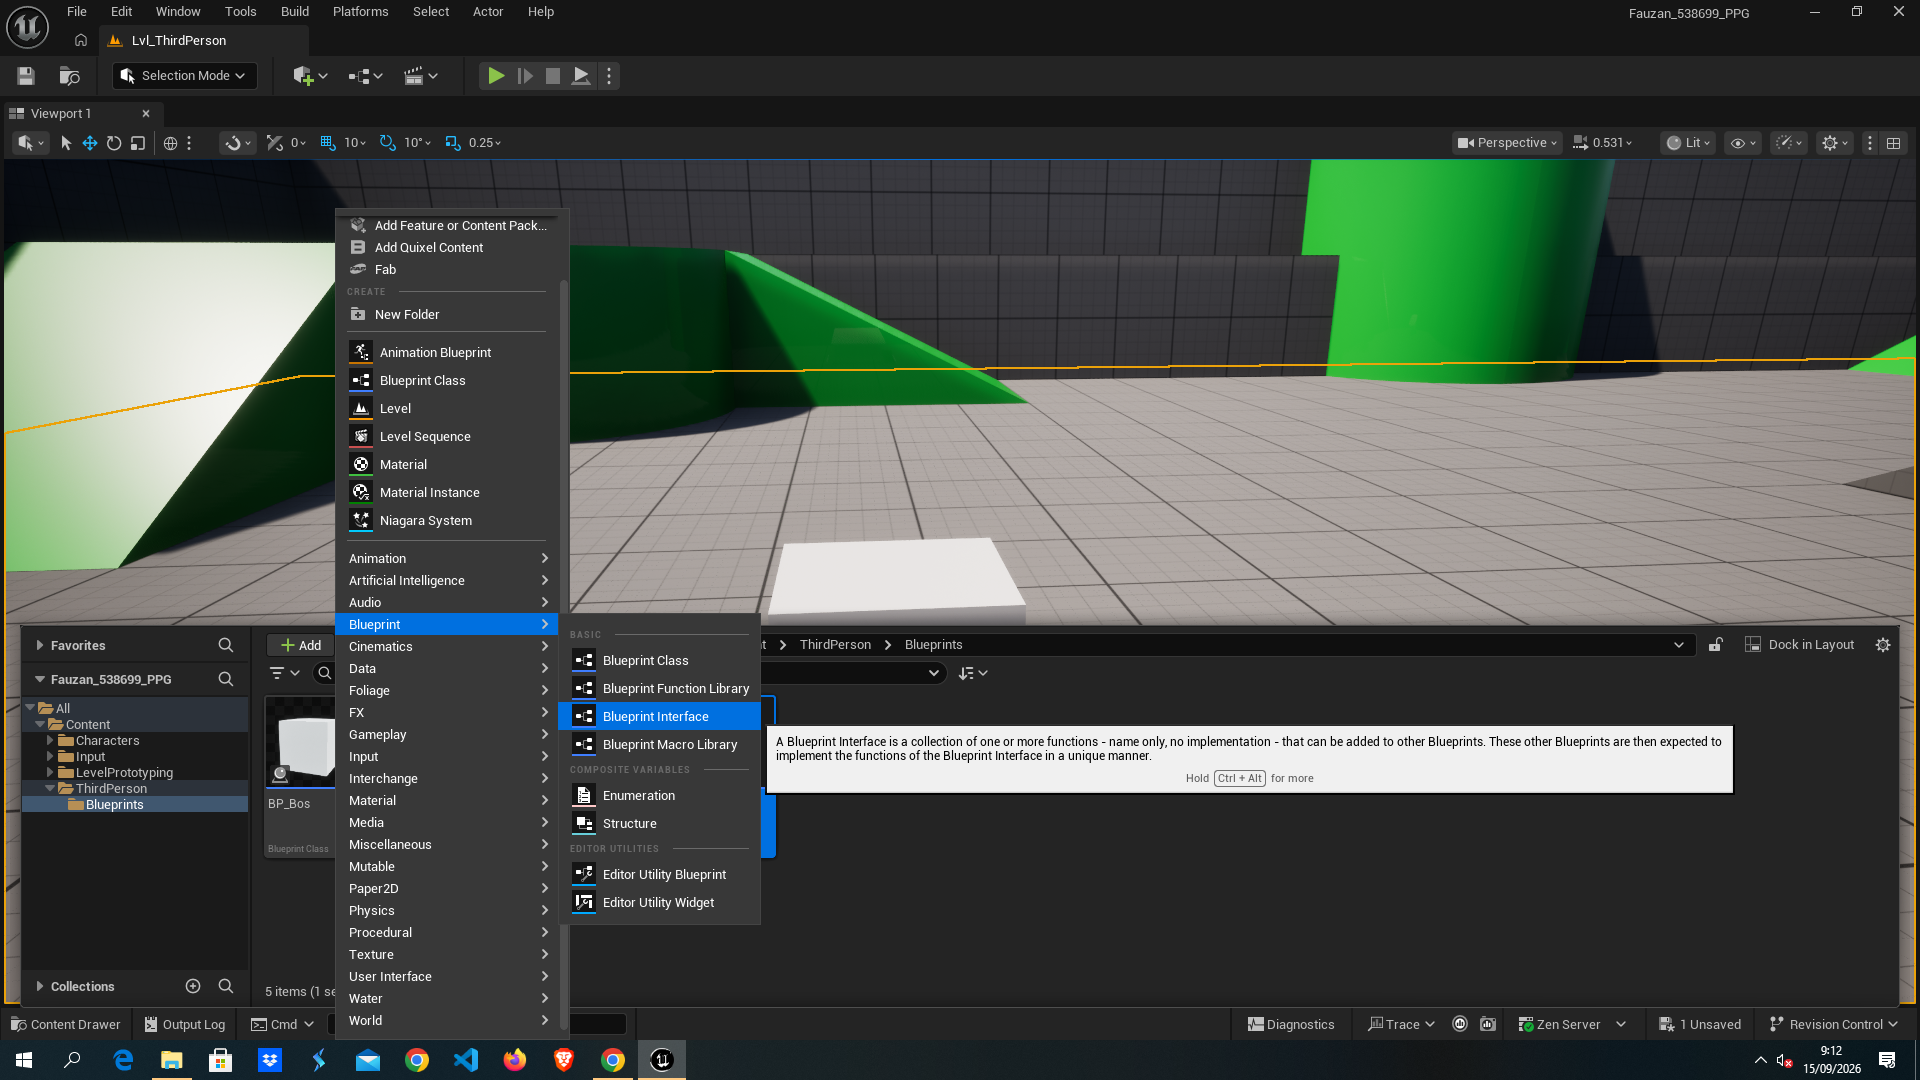
\includegraphics[width=0.8\textwidth]{resource/Dokumentasi/13.png}
  \caption{Pembuatan Blueprint Interface BPI\_Overlap}
  \label{fig:create-bpi-overlap}
\end{figure}

\par Berdasarkan Gambar \ref{fig:create-bpi-overlap}, saya membuat sebuah aset baru bertipe \textit{Blueprint Interface} di Content Drawer. Dengan mengeklik kanan pada area kosong peramban berkas, saya menavigasi ke subkategori \textit{Blueprints} dan memilih menu \textit{Blueprint Interface}. Aset antarmuka yang baru terbentuk tersebut saya beri nama \texttt{BPI\_Overlap} sesuai dengan konvensi penamaan standar berawalan \texttt{BPI\_}, yang difungsikan sebagai kontrak antarmuka universal bagi seluruh objek yang terlibat dalam peristiwa tabrakan overlap.

\begin{figure}[H]
  \centering
  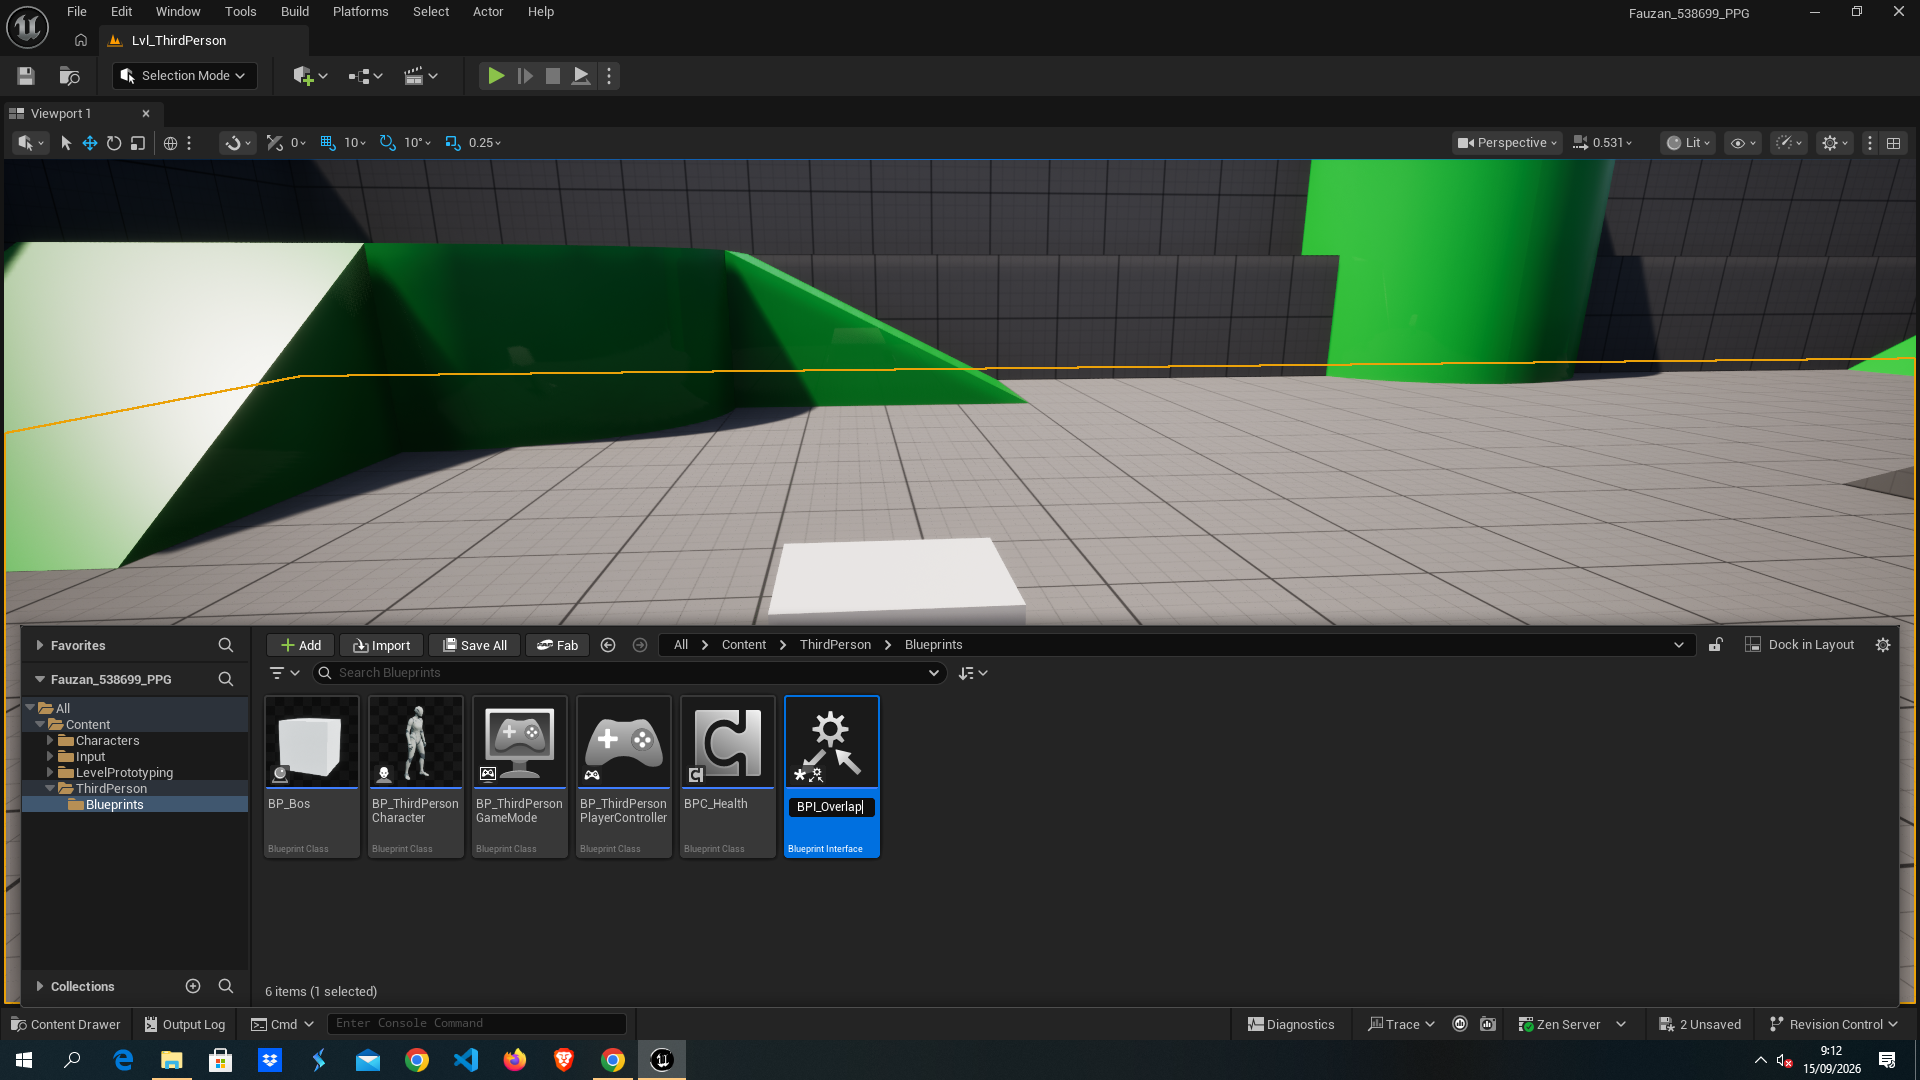
\includegraphics[width=0.8\textwidth]{resource/Dokumentasi/14.png}
  \caption{Pembuatan Deklarasi Fungsi TakeDamage pada BPI\_Overlap}
  \label{fig:bpi-takedamage-func}
\end{figure}

\par Pada Gambar \ref{fig:bpi-takedamage-func}, saya membuka editor aset \texttt{BPI\_Overlap} dan mengamati panel \textit{Functions} di sebelah kiri. Secara baku, sebuah antarmuka menyediakan satu fungsi kosong; saya mengubah nama fungsi tersebut menjadi \texttt{TakeDamage}. Perlu ditegaskan bahwa di dalam sebuah \textit{Blueprint Interface}, fungsi yang dideklarasikan murni bertindak sebagai tanda tangan metode (\textit{method signature}) tanpa memuat badan implementasi visual scripting apapun di dalamnya.

\begin{figure}[H]
  \centering
  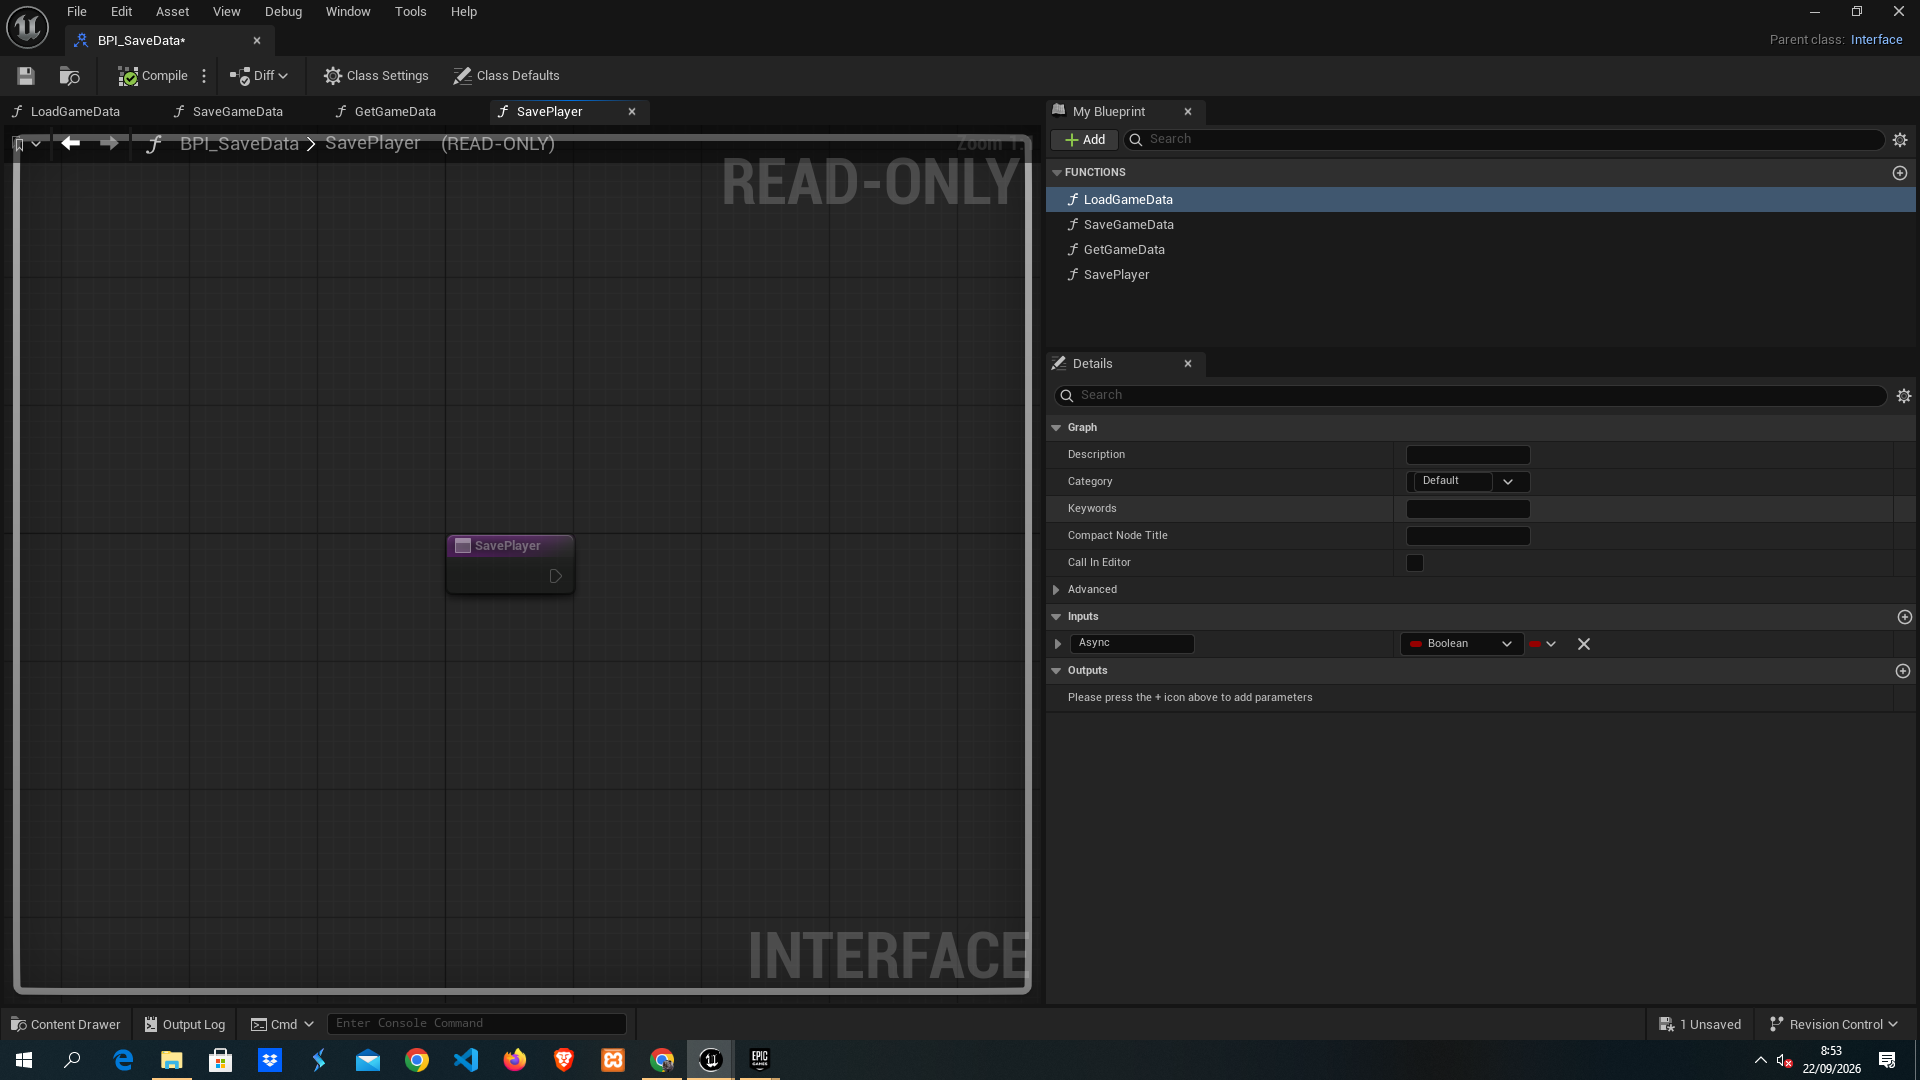
\includegraphics[width=0.8\textwidth]{resource/Dokumentasi/15.png}
  \caption{Konfigurasi Parameter Masukan AmountDamage pada TakeDamage}
  \label{fig:bpi-takedamage-input}
\end{figure}

\par Melanjutkan perancangan kontrak antarmuka, Gambar \ref{fig:bpi-takedamage-input} memperlihatkan konfigurasi parameter masukan pada fungsi \texttt{TakeDamage}. Melalui panel \textit{Details} di sisi kanan editor, saya mengeklik tombol \textit{+ Add} pada kategori \textit{Inputs}, lalu memberi nama parameter masukan tersebut \texttt{AmountDamage} dengan tipe data \textit{Float}. Argumen numerik ini dirancang secara khusus untuk mengalirkan data besaran nilai kerusakan dari aktor pemancar sinyal tabrakan menuju ke aktor target penerima interaksi.

\begin{figure}[H]
  \centering
  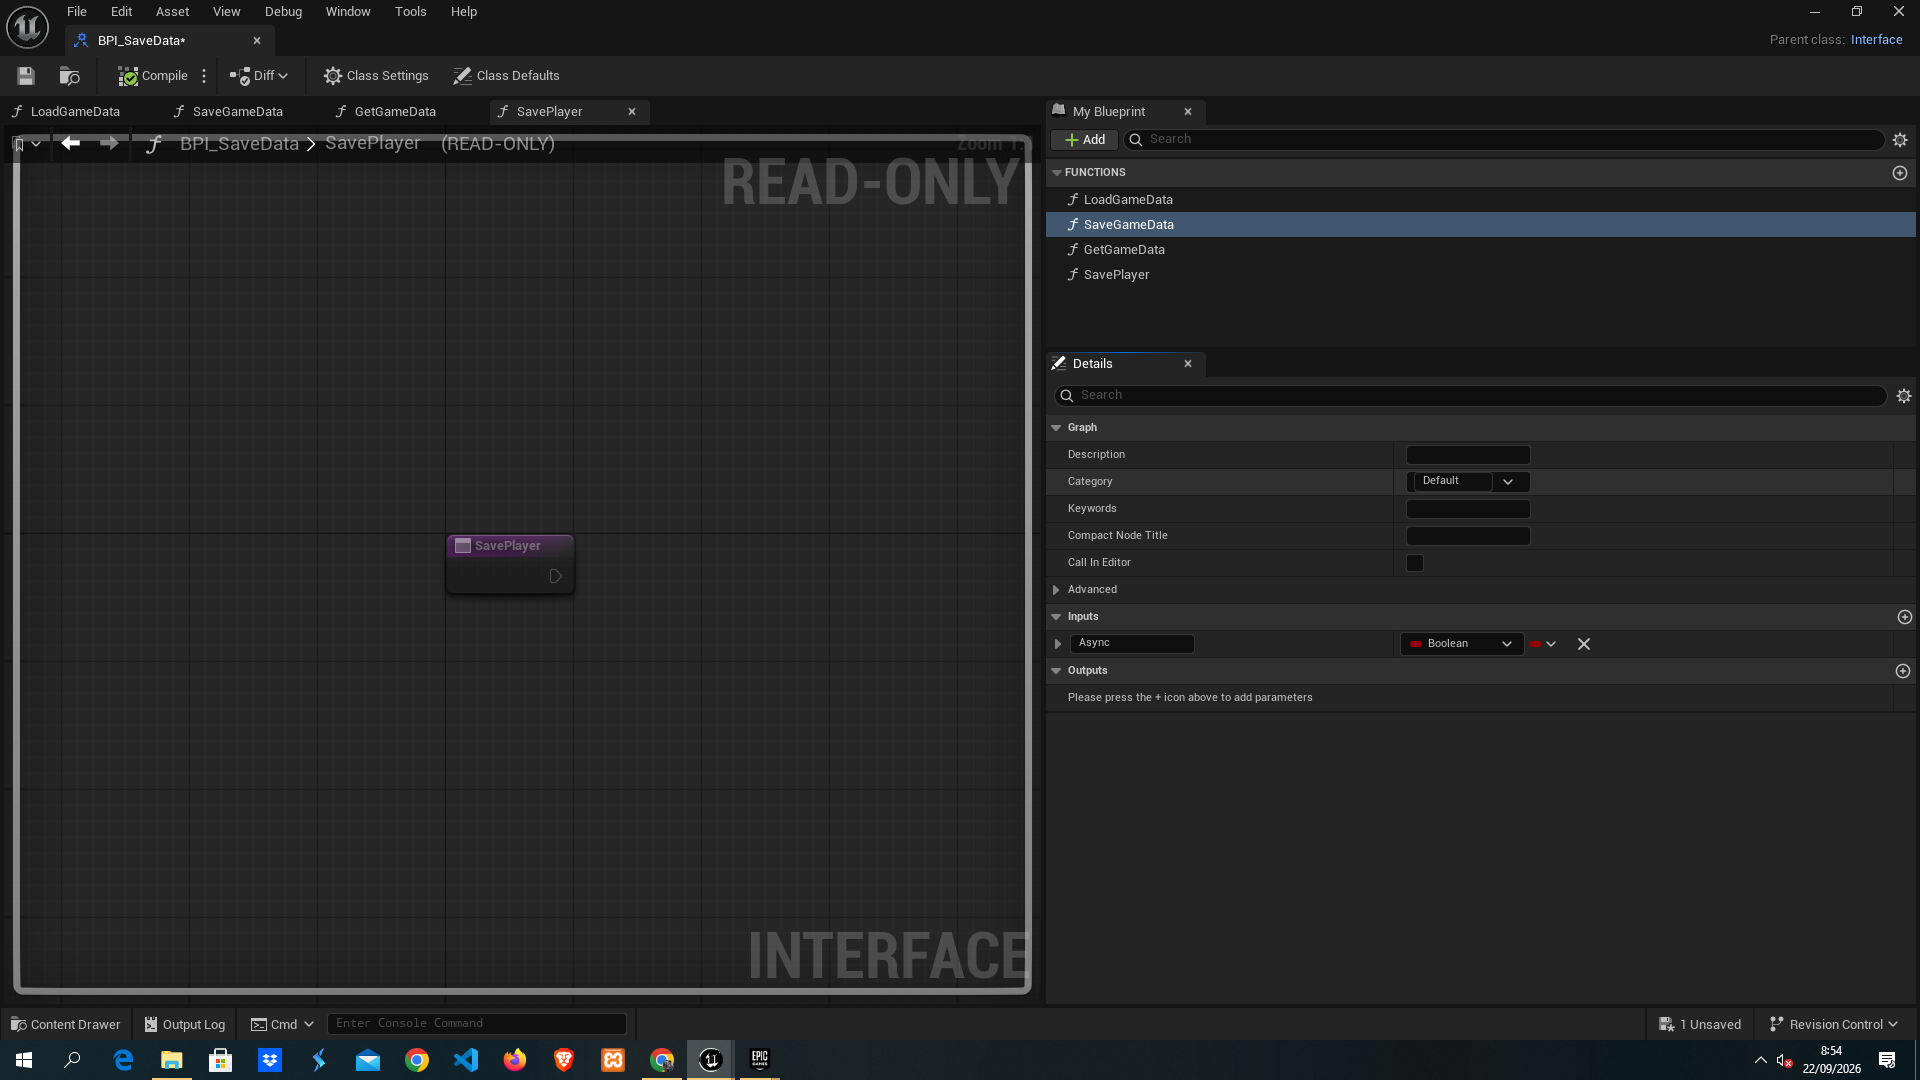
\includegraphics[width=0.8\textwidth]{resource/Dokumentasi/16.png}
  \caption{Kompilasi dan Penyimpanan Aset BPI\_Overlap}
  \label{fig:bpi-compile}
\end{figure}

\par Berdasarkan Gambar \ref{fig:bpi-compile}, setelah mendeklarasikan fungsi dan parameter masukannya, saya menekan tombol \textit{Compile} dan \textit{Save} pada bilah alat kerja utama editor antarmuka. Tanda centang hijau pada tombol kompilasi mengonfirmasikan bahwa struktur kontrak antarmuka \texttt{BPI\_Overlap} telah berhasil terdaftar secara valid dalam basis data proyek Unreal Engine dan siap diimplementasikan oleh kelas-kelas aktor dalam permainan.

\begin{figure}[H]
  \centering
  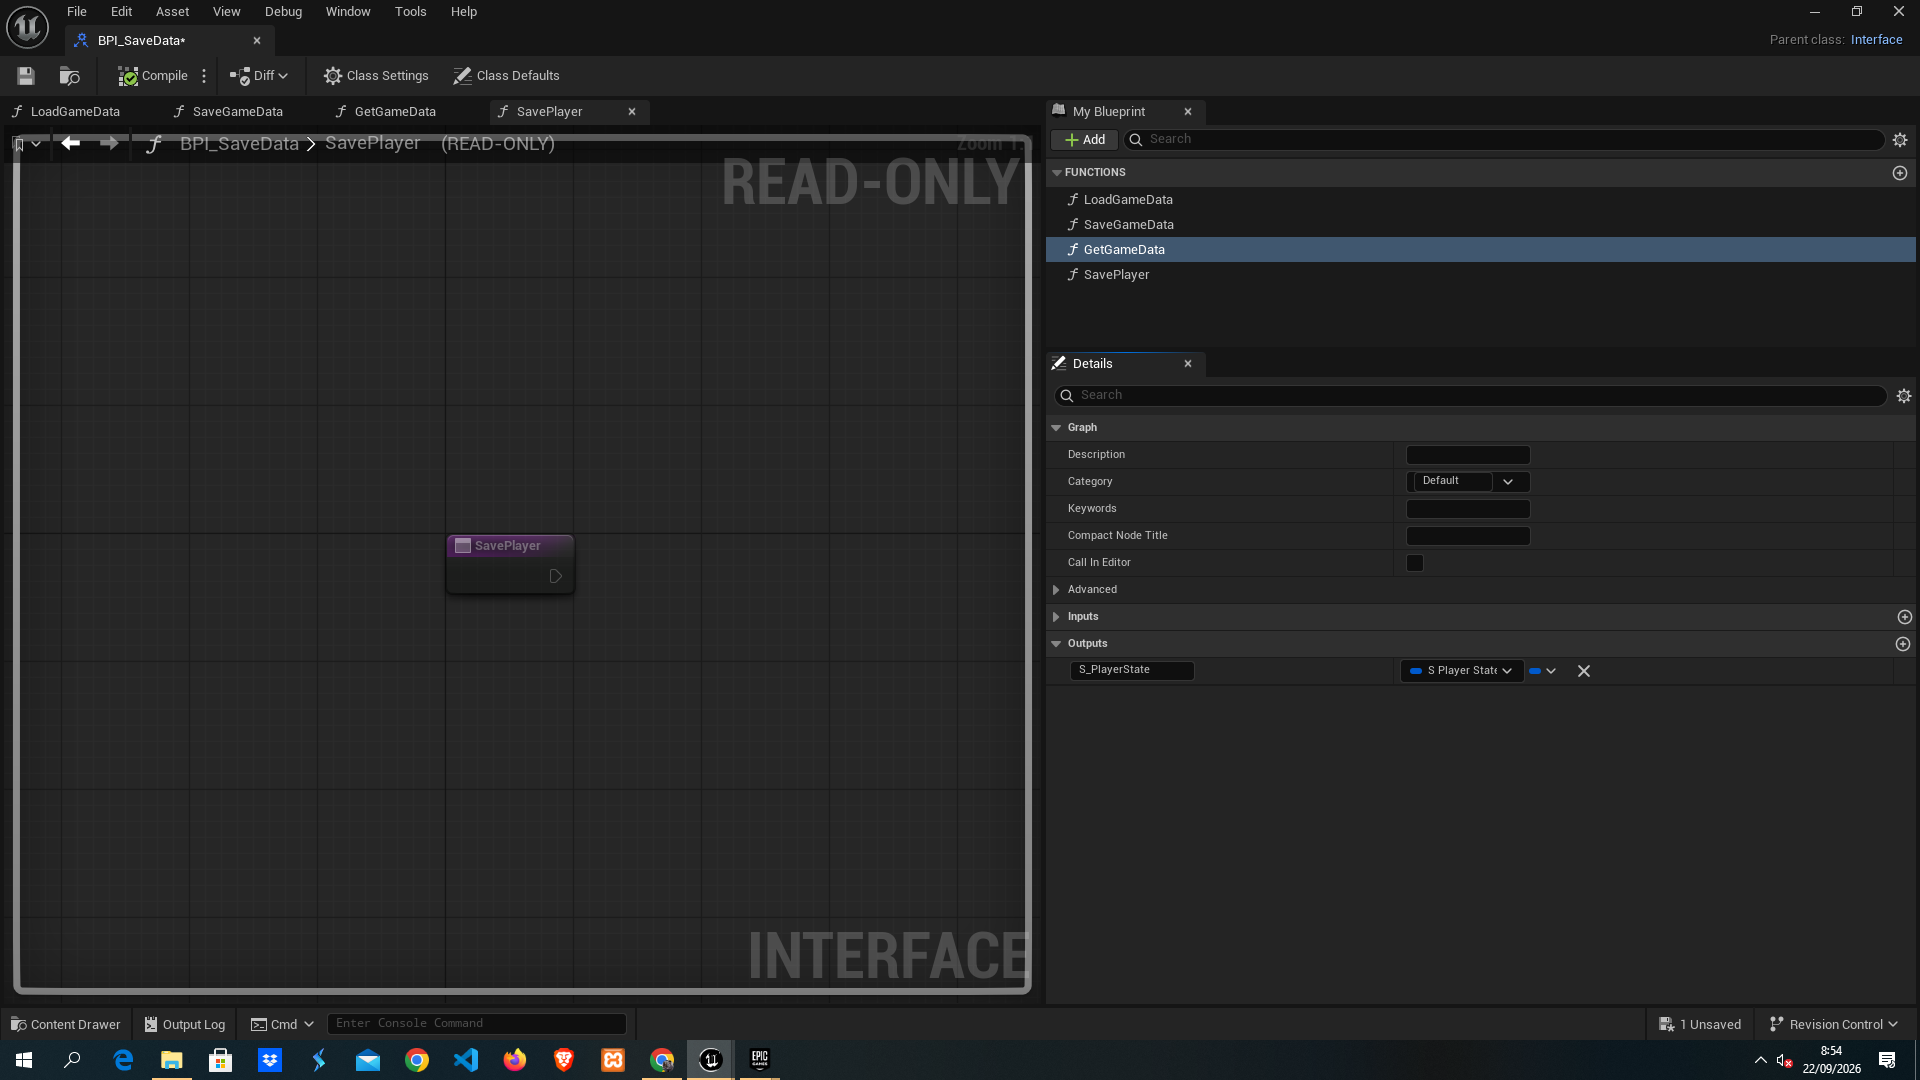
\includegraphics[width=0.8\textwidth]{resource/Dokumentasi/17.png}
  \caption{Membuka Pengaturan Class Settings pada BP\_ThirdPersonCharacter}
  \label{fig:open-class-settings}
\end{figure}

\par Pada Gambar \ref{fig:open-class-settings}, saya kembali membuka editor karakter \texttt{BP\_ThirdPersonCharacter} dan mengeklik tombol \textit{Class Settings} pada bilah alat kerja utama di bagian atas kanvas kerja. Aksi ini mengalihkan panel \textit{Details} di sisi kanan layar untuk menampilkan properti konfigurasi kelas secara mendasar, termasuk pengaturan kelas induk, opsi replikasi jaringan, serta daftar antarmuka yang diadopsi oleh karakter.

\begin{figure}[H]
  \centering
  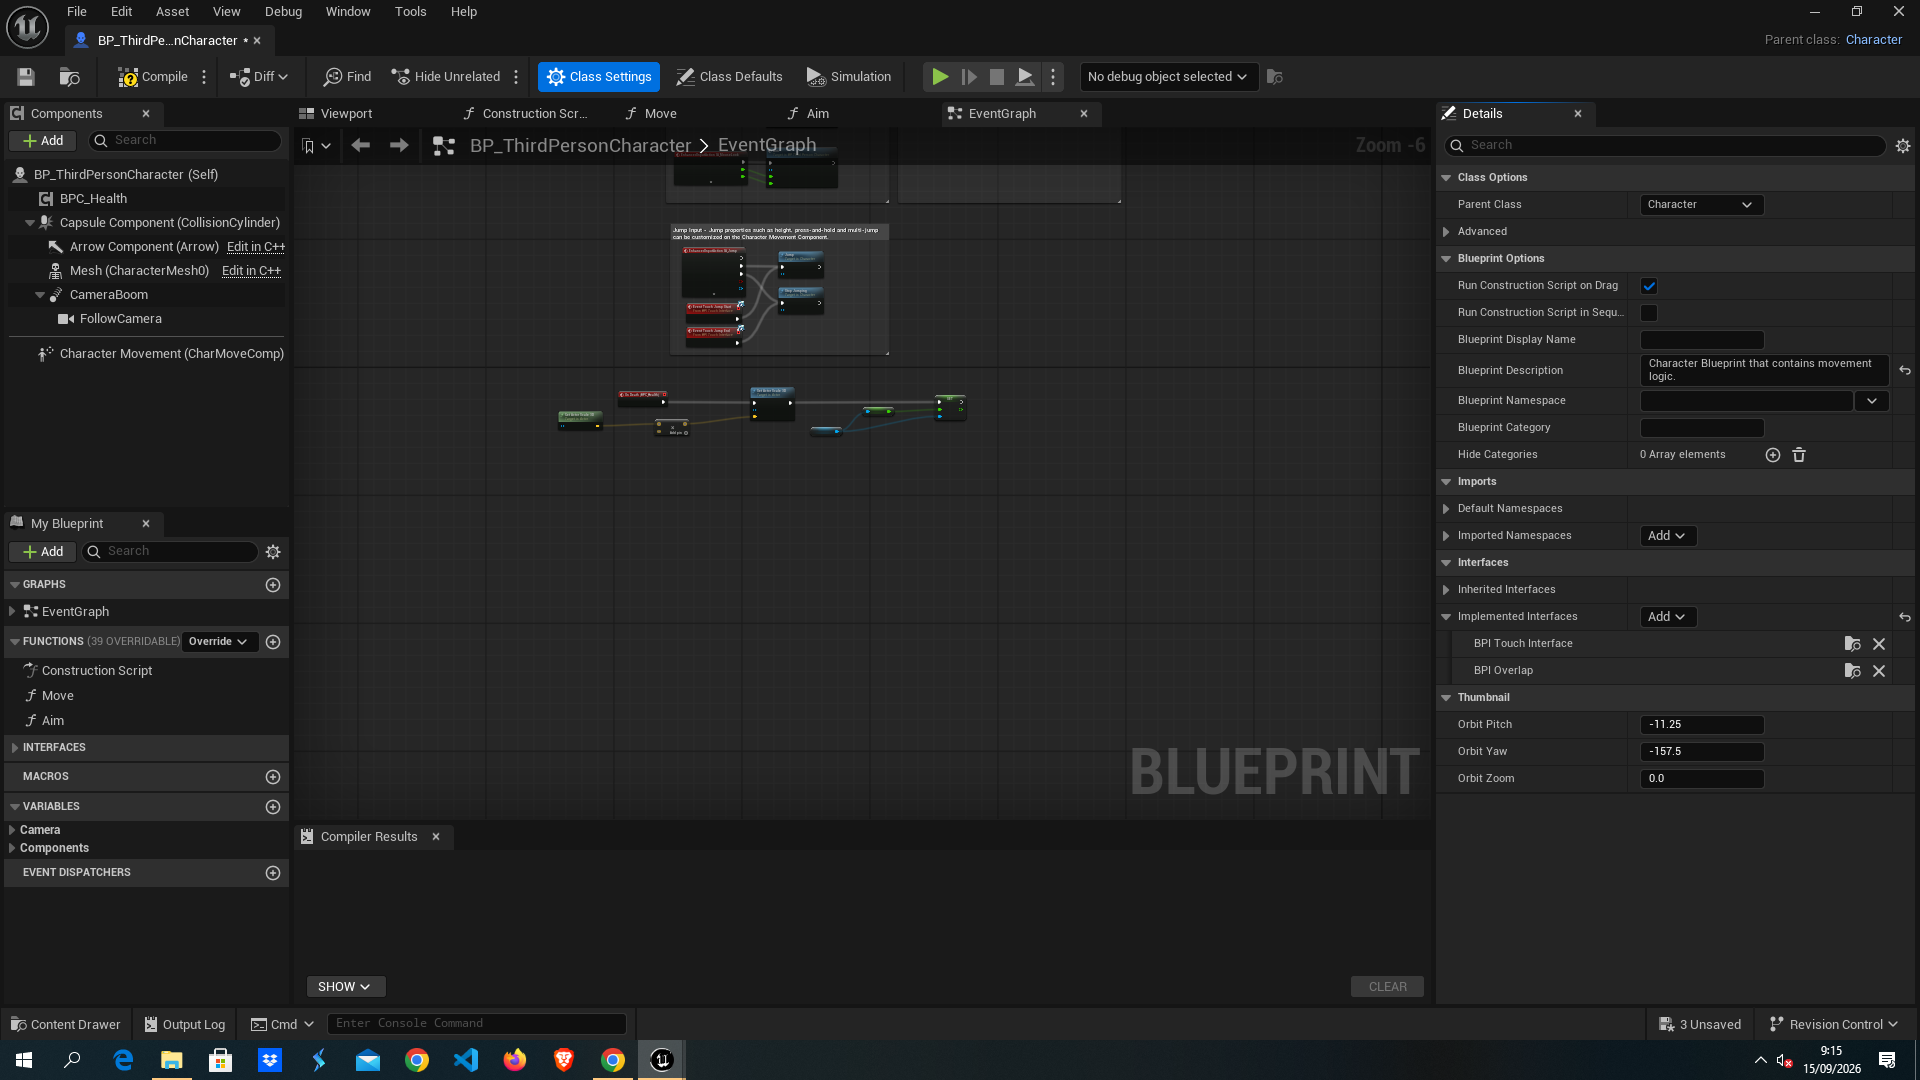
\includegraphics[width=0.8\textwidth]{resource/Dokumentasi/18.png}
  \caption{Menambahkan BPI\_Overlap ke Implemented Interfaces}
  \label{fig:add-implemented-interface}
\end{figure}

\par Langkah berlanjut dengan mendaftarkan kontrak antarmuka pada karakter sebagaimana ditunjukkan pada Gambar \ref{fig:add-implemented-interface}. Pada panel \textit{Details > Interfaces}, saya menekan tombol \textit{Add} di sebelah daftar \textit{Implemented Interfaces}, kemudian mencari dan memilih aset \texttt{BPI\_Overlap}. Dengan menambahkan antarmuka ini, \texttt{BP\_ThirdPersonCharacter} secara resmi terdaftar sebagai kelas yang mampu mengenali dan merespons pesan fungsi yang dikirimkan melalui saluran \texttt{BPI\_Overlap}.

\begin{figure}[H]
  \centering
  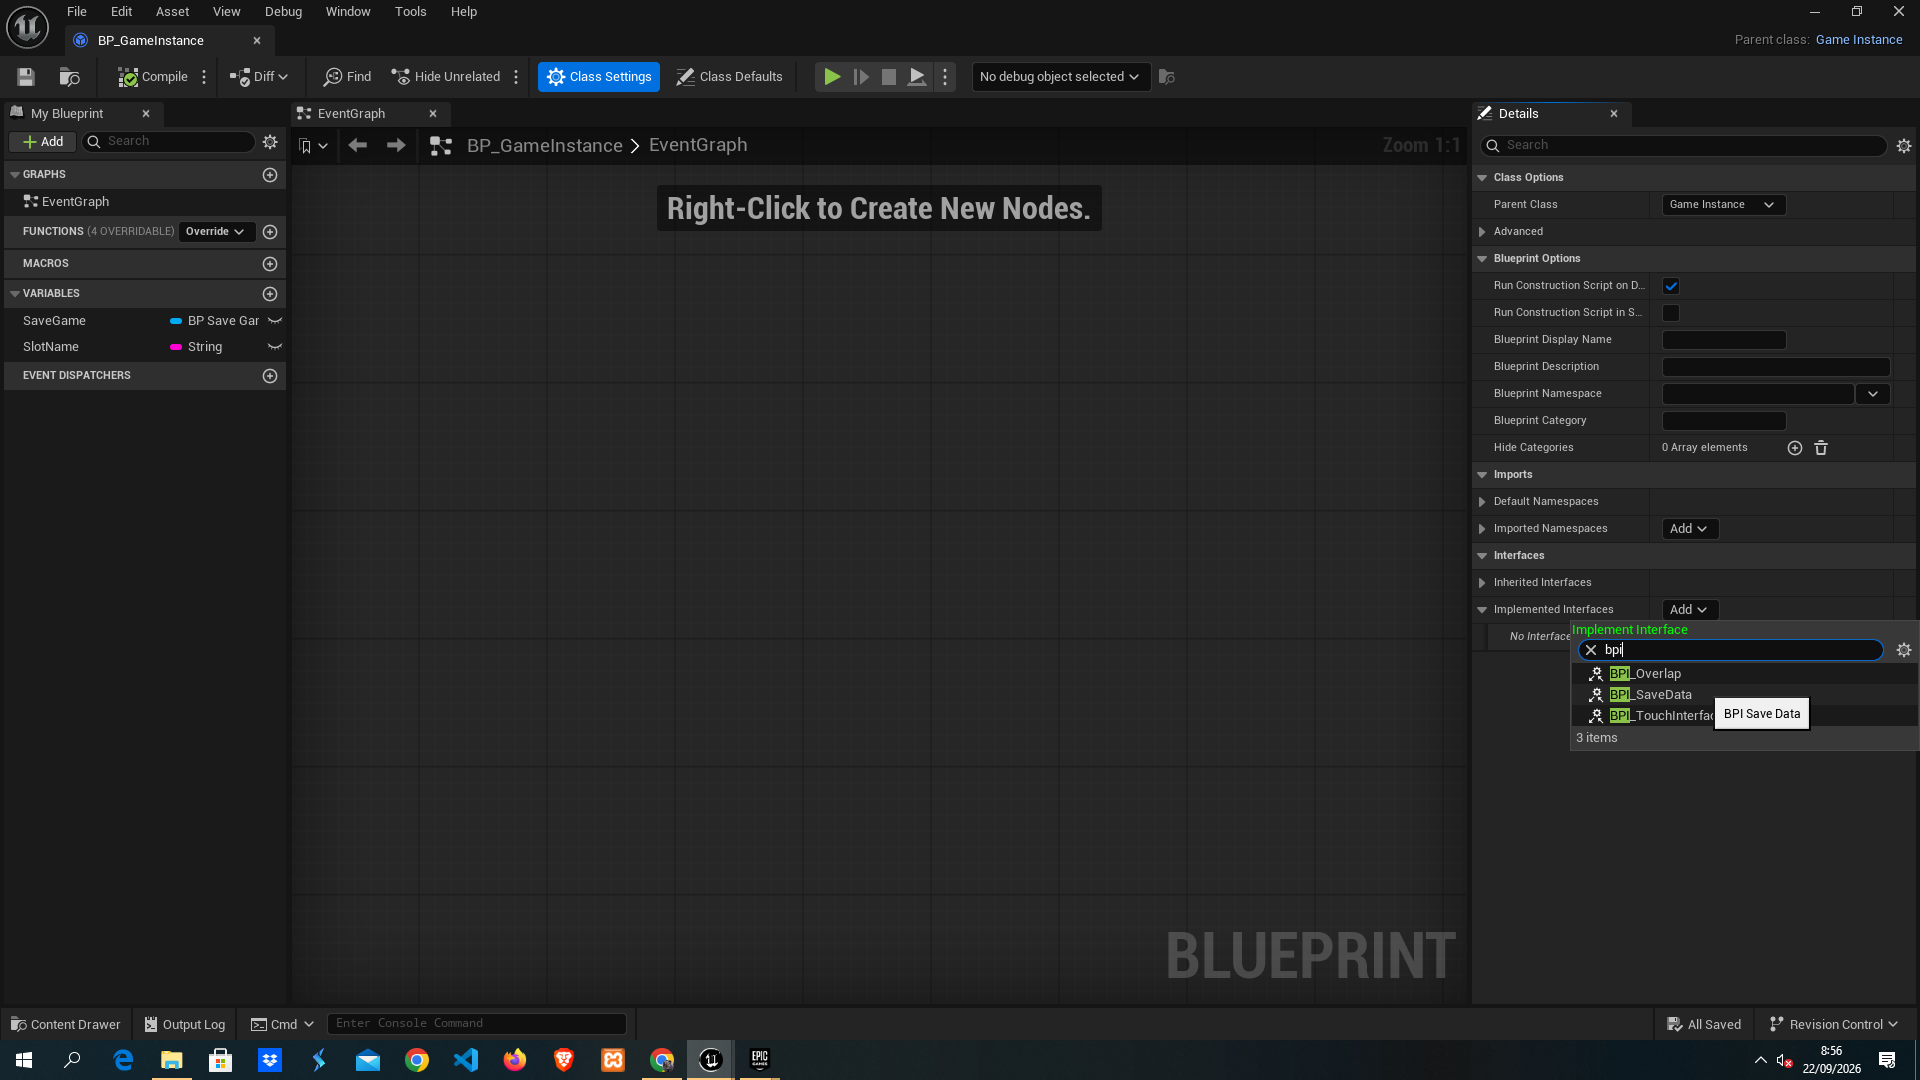
\includegraphics[width=0.8\textwidth]{resource/Dokumentasi/19.png}
  \caption{Implementasi Event TakeDamage pada Event Graph Karakter}
  \label{fig:implement-event-takedamage}
\end{figure}

\par Berdasarkan Gambar \ref{fig:implement-event-takedamage}, setelah antarmuka terdaftar, saya beralih kembali ke \textit{Event Graph} milik \texttt{BP\_ThirdPersonCharacter}. Melalui menu konteks klik kanan, saya menavigasi ke kategori \textit{Add Event for Interface} dan memilih node \texttt{Event TakeDamage}. Node kejadian ini memiliki ikon panah antarmuka berwarna kuning di sudut kiri atasnya dan menyediakan pin keluaran parameter \texttt{AmountDamage} yang siap memproses nilai kerusakan setiap kali pesan antarmuka dipanggil oleh objek lain.

\begin{figure}[H]
  \centering
  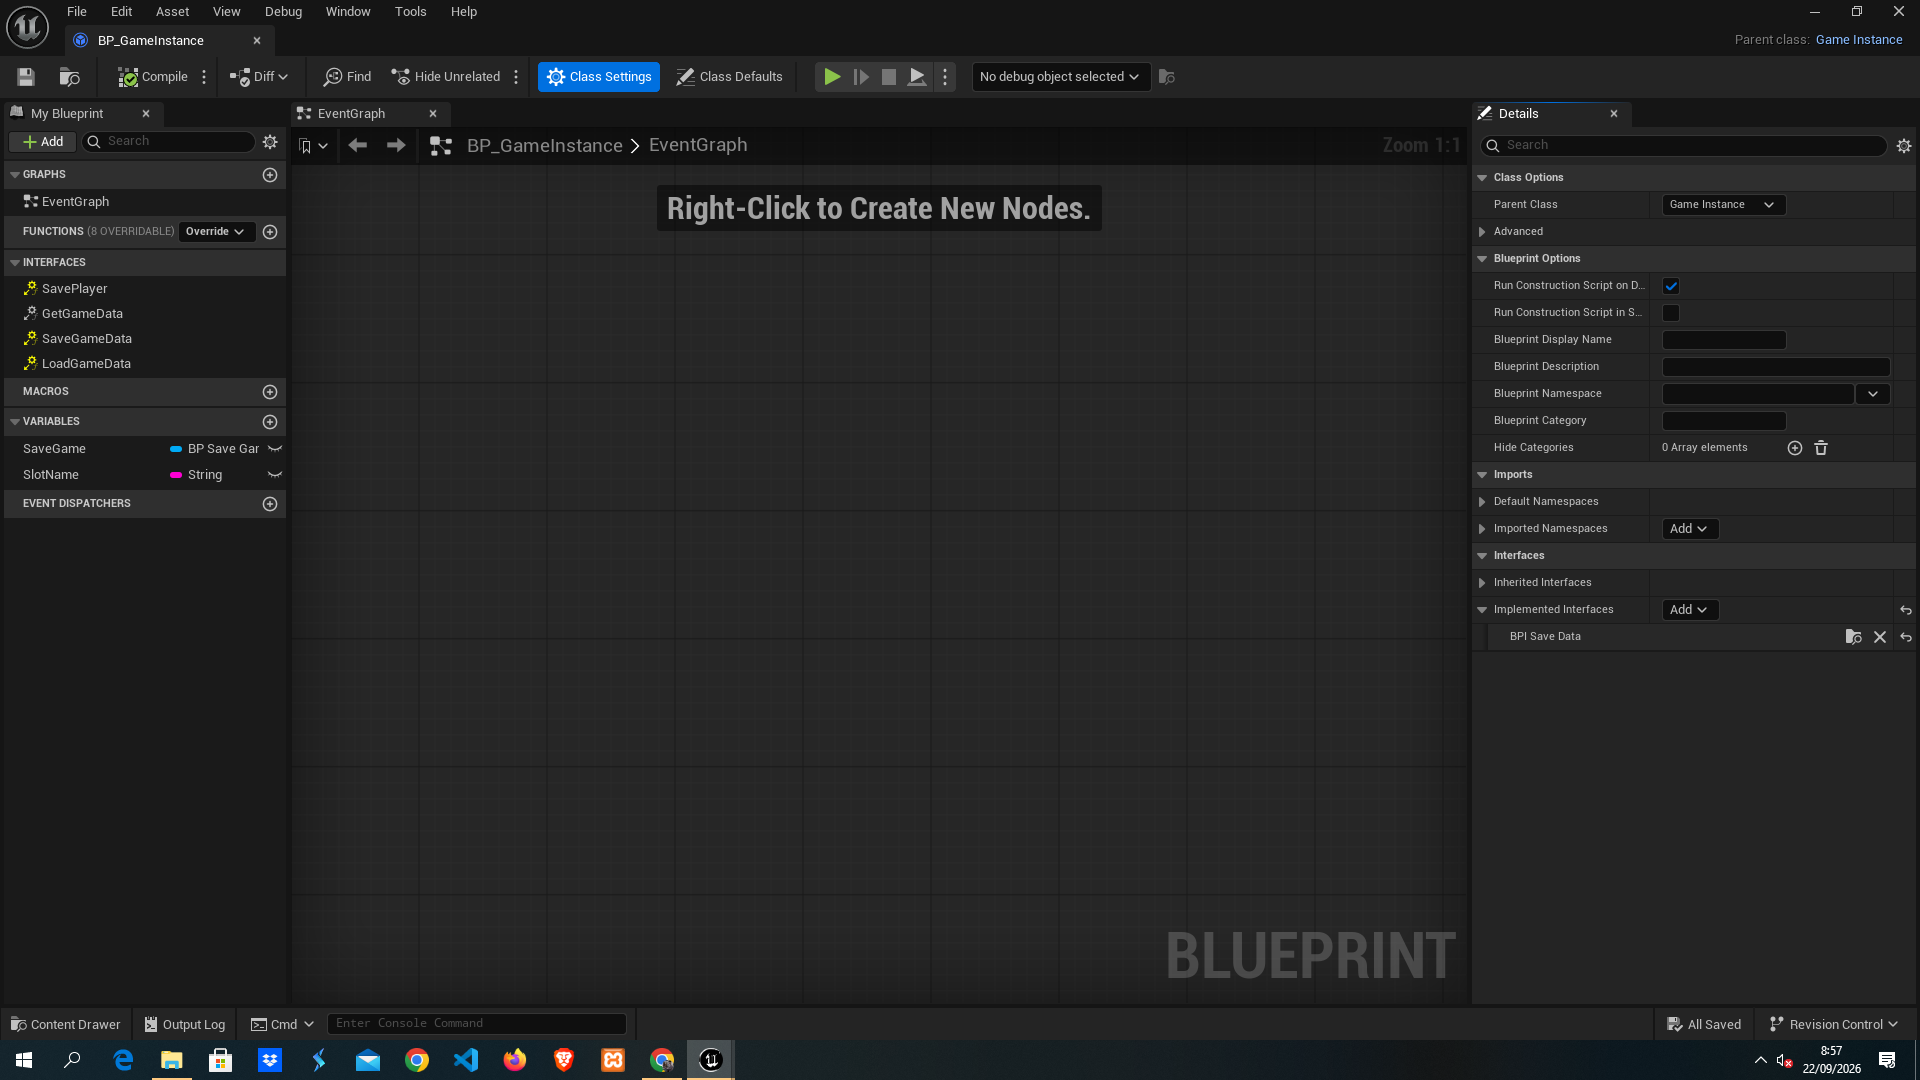
\includegraphics[width=0.8\textwidth]{resource/Dokumentasi/20.png}
  \caption{Menghubungkan Event TakeDamage ke ModifyHealth Milik BPC\_Health}
  \label{fig:connect-takedamage-modifyhealth}
\end{figure}

\par Pada Gambar \ref{fig:connect-takedamage-modifyhealth}, saya menghubungkan alur eksekusi dari node \texttt{Event TakeDamage} menuju ke fungsi \texttt{ModifyHealth} milik komponen \texttt{BPC\_Health}. Karena parameter \texttt{AmountDamage} membawa nilai positif sedangkan pengurangan kesehatan memerlukan masukan bernilai negatif, saya menghubungkan pin \texttt{AmountDamage} ke operator perkalian (\textit{Multiply Float * Float}) dan mengalikannya dengan angka konstan -1.0. Hasil pembalikan tanda tersebut kemudian dialirkan ke pin input \texttt{Amount} pada node \texttt{ModifyHealth}, sehingga setiap pesan kerusakan yang diterima karakter akan langsung memicu pengurangan nilai darah secara akurat.

\subsection{Perancangan Aktor Pemicu Tabrakan (BP\_Collision) dan Pengaturan Visibilitas Box}

\par Pada subbab ini, saya merancang sebuah entitas aktor mandiri dalam bentuk objek pemicu tabrakan (\texttt{BP\_Collision}). Aktor ini bertindak sebagai perangkap lingkungan yang mendeteksi keberadaan karakter pemain di dalam ruang spasialnya dan secara otomatis memancarkan pesan kerusakan melalui kontrak antarmuka yang telah dibuat sebelumnya.

\begin{figure}[H]
  \centering
  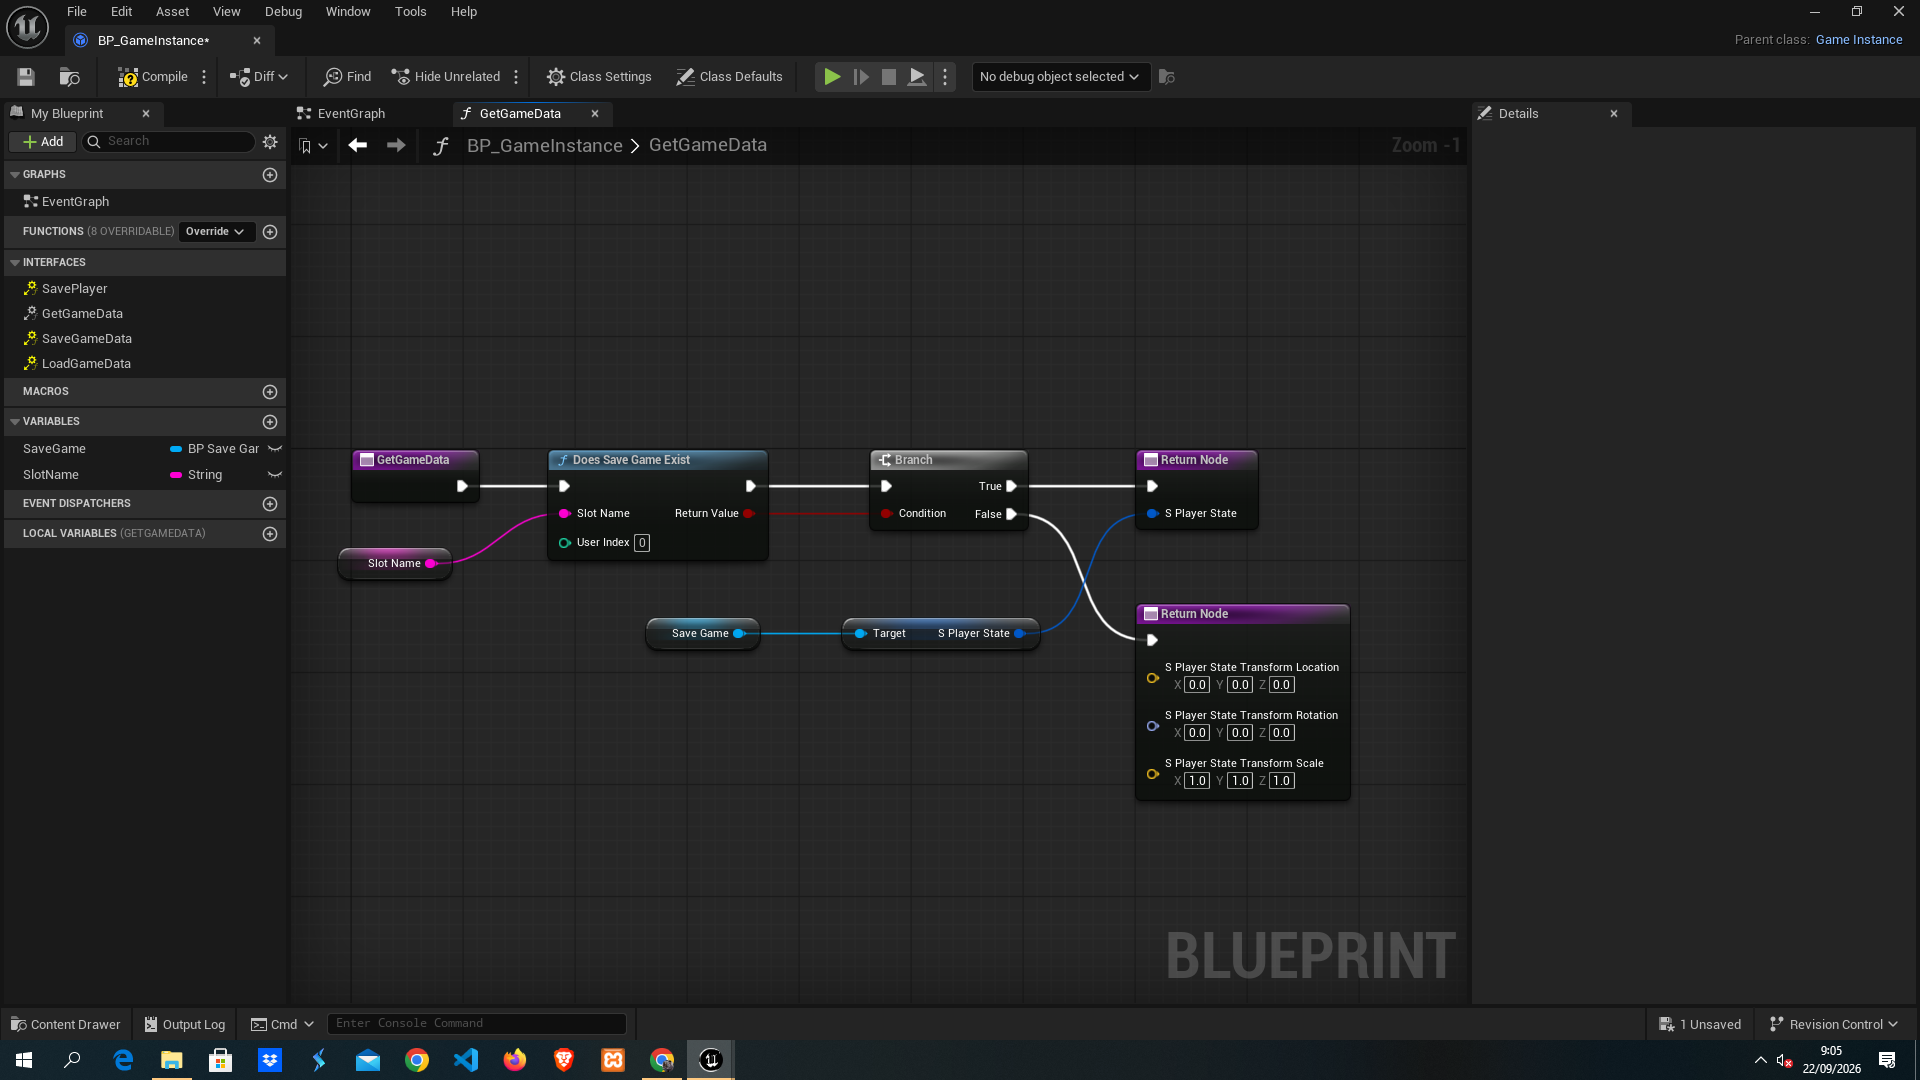
\includegraphics[width=0.8\textwidth]{resource/Dokumentasi/21.png}
  \caption{Pembuatan Blueprint Class Baru Bertipe Actor BP\_Collision}
  \label{fig:create-bp-collision}
\end{figure}

\par Berdasarkan Gambar \ref{fig:create-bp-collision}, saya membuat sebuah \textit{Blueprint Class} baru berbasis kelas induk \textit{Actor} melalui menu klik kanan pada Content Drawer. Aset objek lingkungan ini saya beri nama \texttt{BP\_Collision} dengan menggunakan prefiks \texttt{BP\_}. Aktor ini dirancang murni sebagai volume pemicu tabrakan tanpa membutuhkan komponen jaring poligon statis (\textit{static mesh}) yang rumit.

\begin{figure}[H]
  \centering
  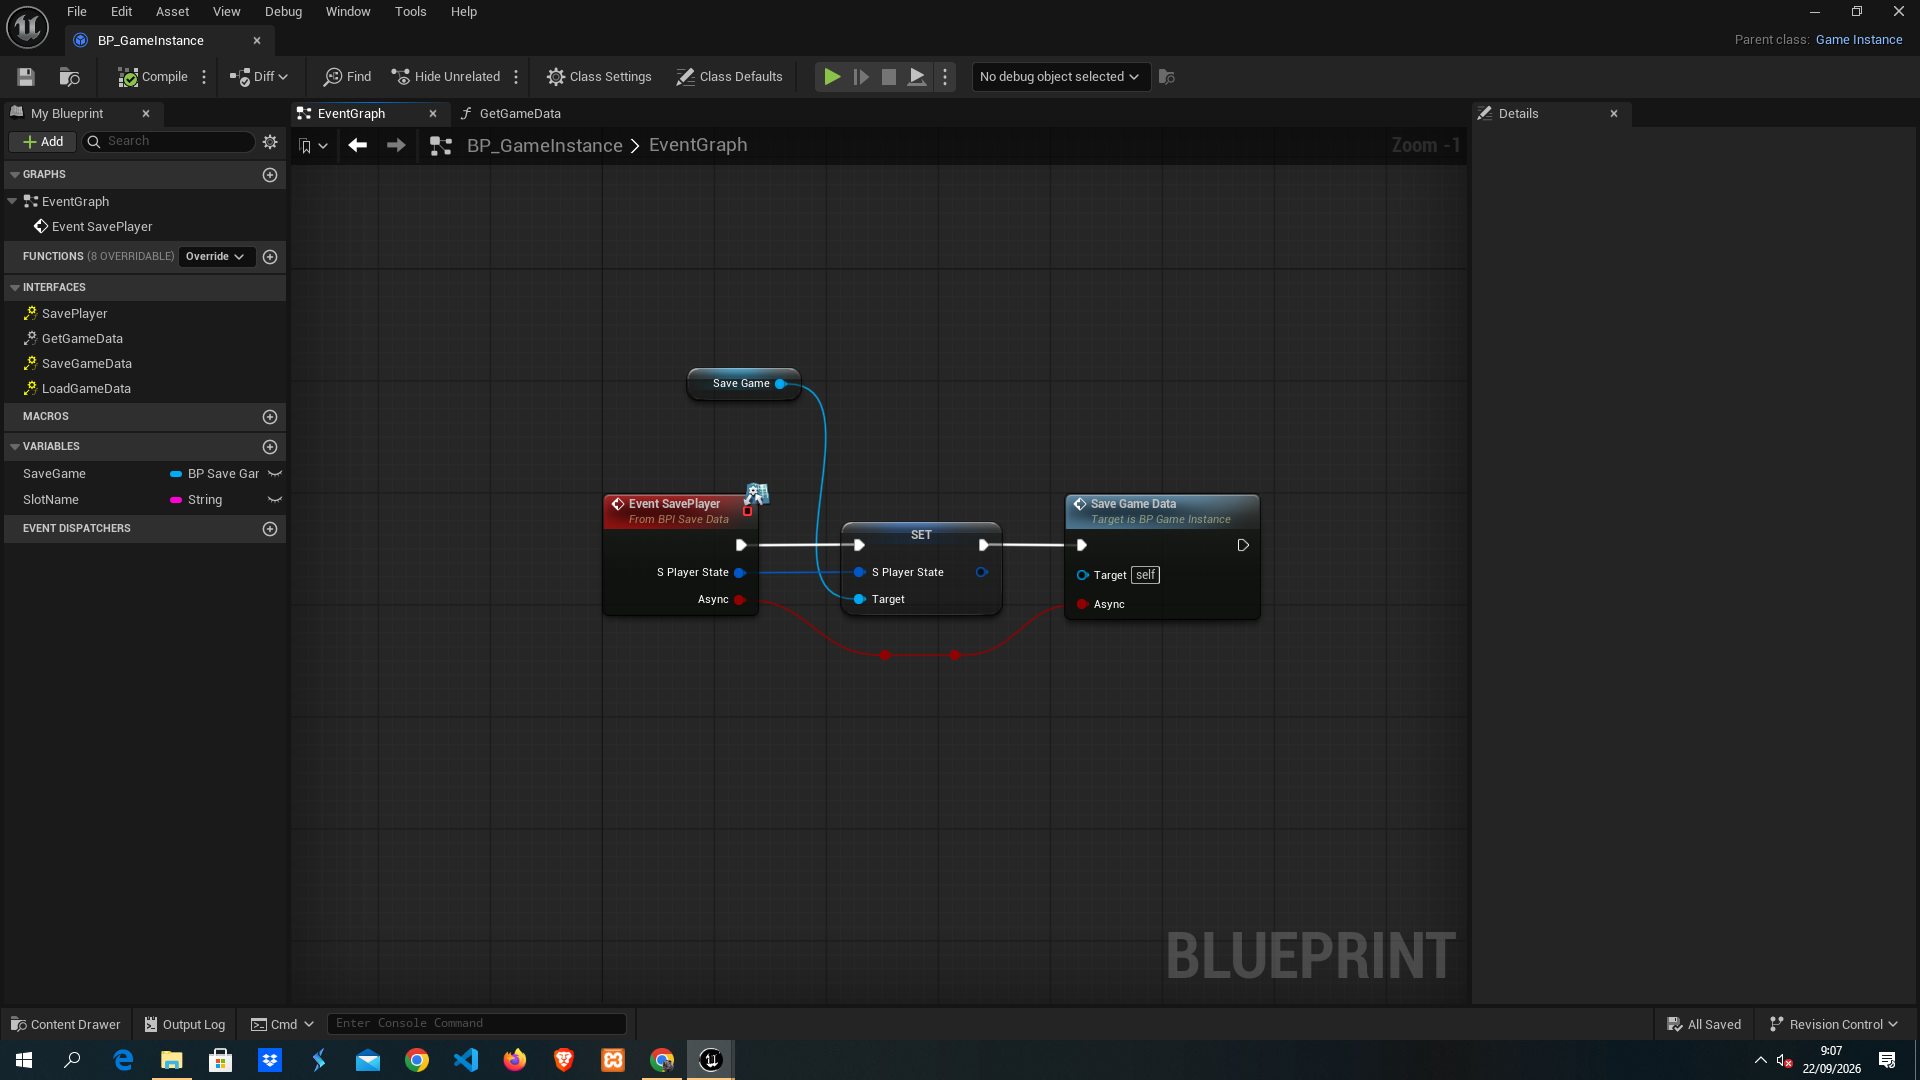
\includegraphics[width=0.8\textwidth]{resource/Dokumentasi/22.png}
  \caption{Tampilan Awal Viewport BP\_Collision}
  \label{fig:viewport-bp-collision-initial}
\end{figure}

\par Pada Gambar \ref{fig:viewport-bp-collision-initial}, saya membuka editor \texttt{BP\_Collision} dan memeriksa tampilan tab \textit{Viewport}. Pada kondisi awal pembuatan, aktor ini hanya memuat sebuah komponen bawaan sistem bernama \texttt{DefaultSceneRoot} berupa bola putih kecil yang berfungsi sebagai titik acuan transformasi spasial koordinat tiga dimensi (lokasi, rotasi, dan skala) tanpa adanya batas fisik tabrakan maupun representasi visual apapun.

\begin{figure}[H]
  \centering
  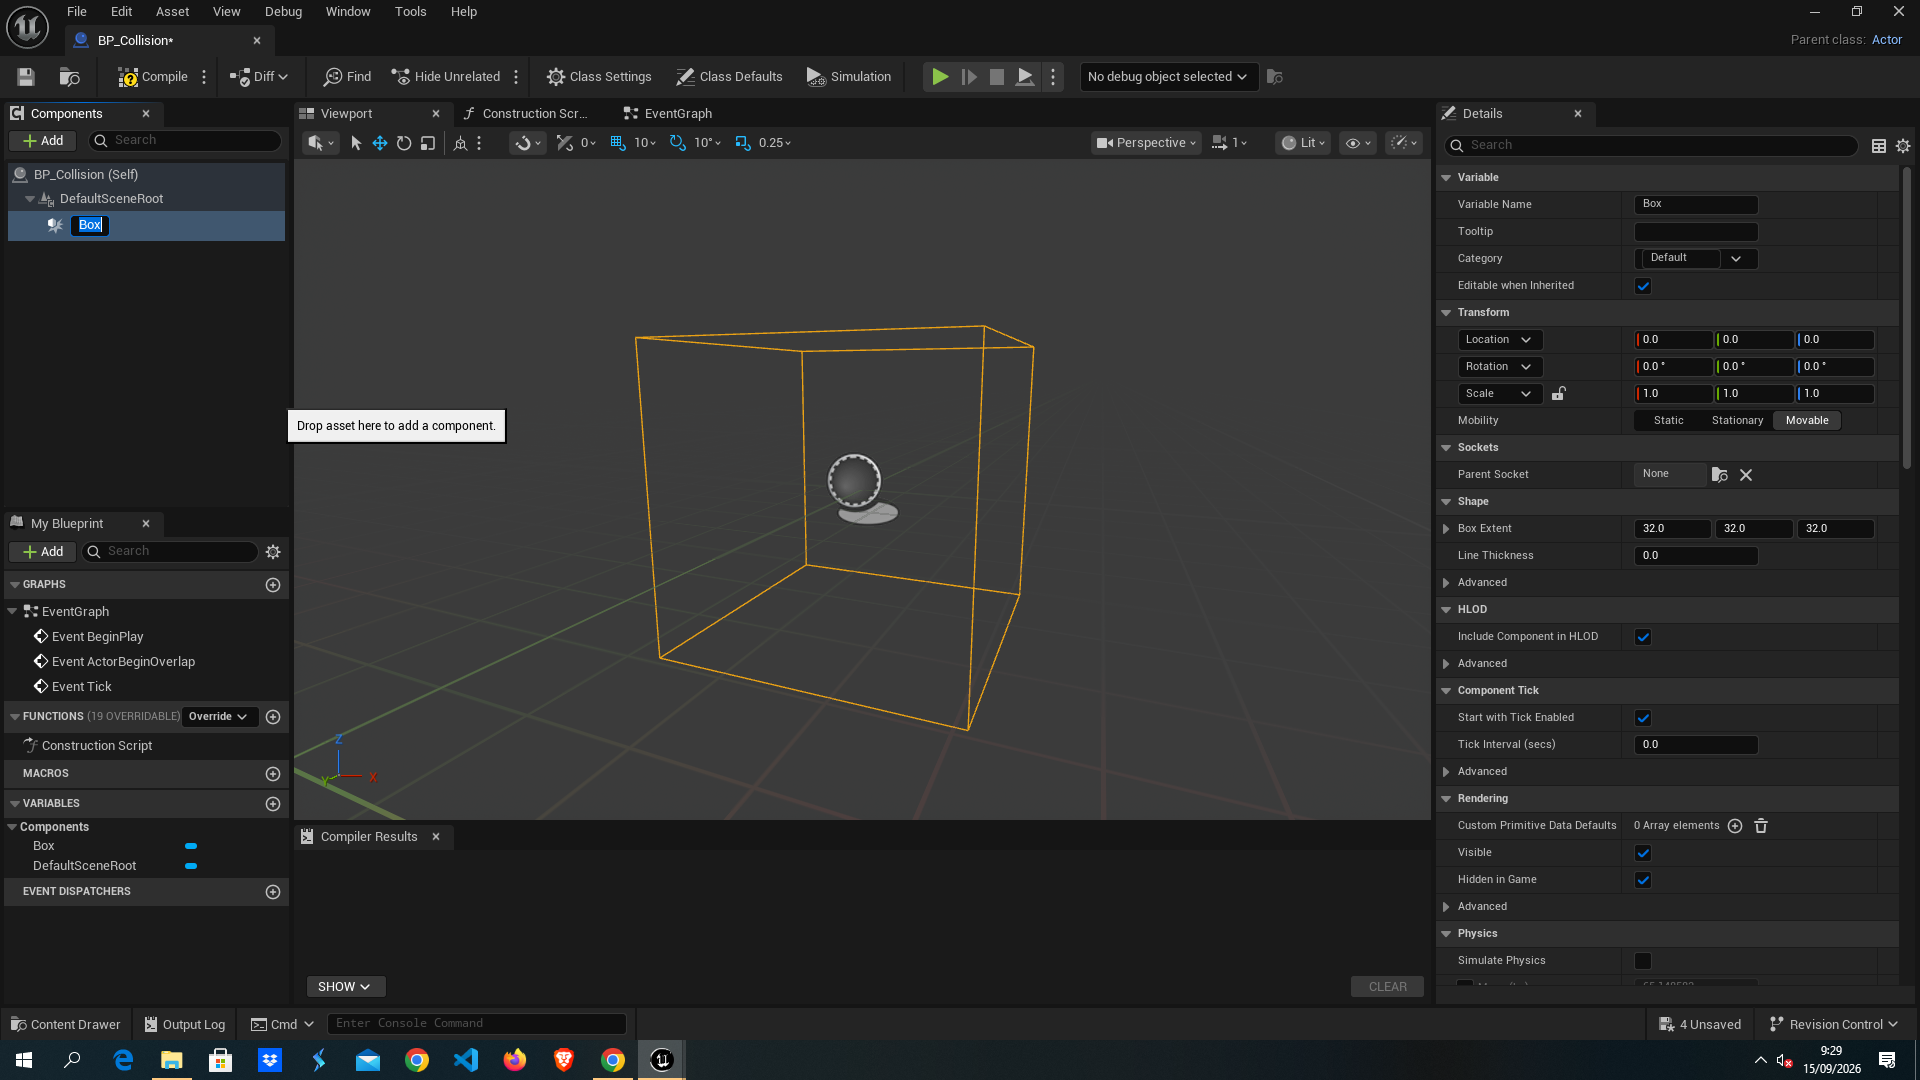
\includegraphics[width=0.8\textwidth]{resource/Dokumentasi/23.png}
  \caption{Penambahan Komponen Box Collision pada BP\_Collision}
  \label{fig:add-box-collision-component}
\end{figure}

\par Langkah berlanjut dengan menambahkan volume pembatas spasial, seperti diperlihatkan pada Gambar \ref{fig:add-box-collision-component}. Pada panel \textit{Components}, saya mengeklik tombol \textit{+ Add}, mencari komponen tabrakan \textit{Box Collision}, dan memberi nama komponen tersebut \texttt{Box}. Komponen ini menghasilkan volume batas tiga dimensi berupa kerangka kawat transparan (\textit{wireframe box}) yang mampu membangkitkan peristiwa tumpang tindih fisik (\textit{overlap event}) seketika batas geometrisnya dilewati oleh aktor lain di dalam permainan.

\begin{figure}[H]
  \centering
  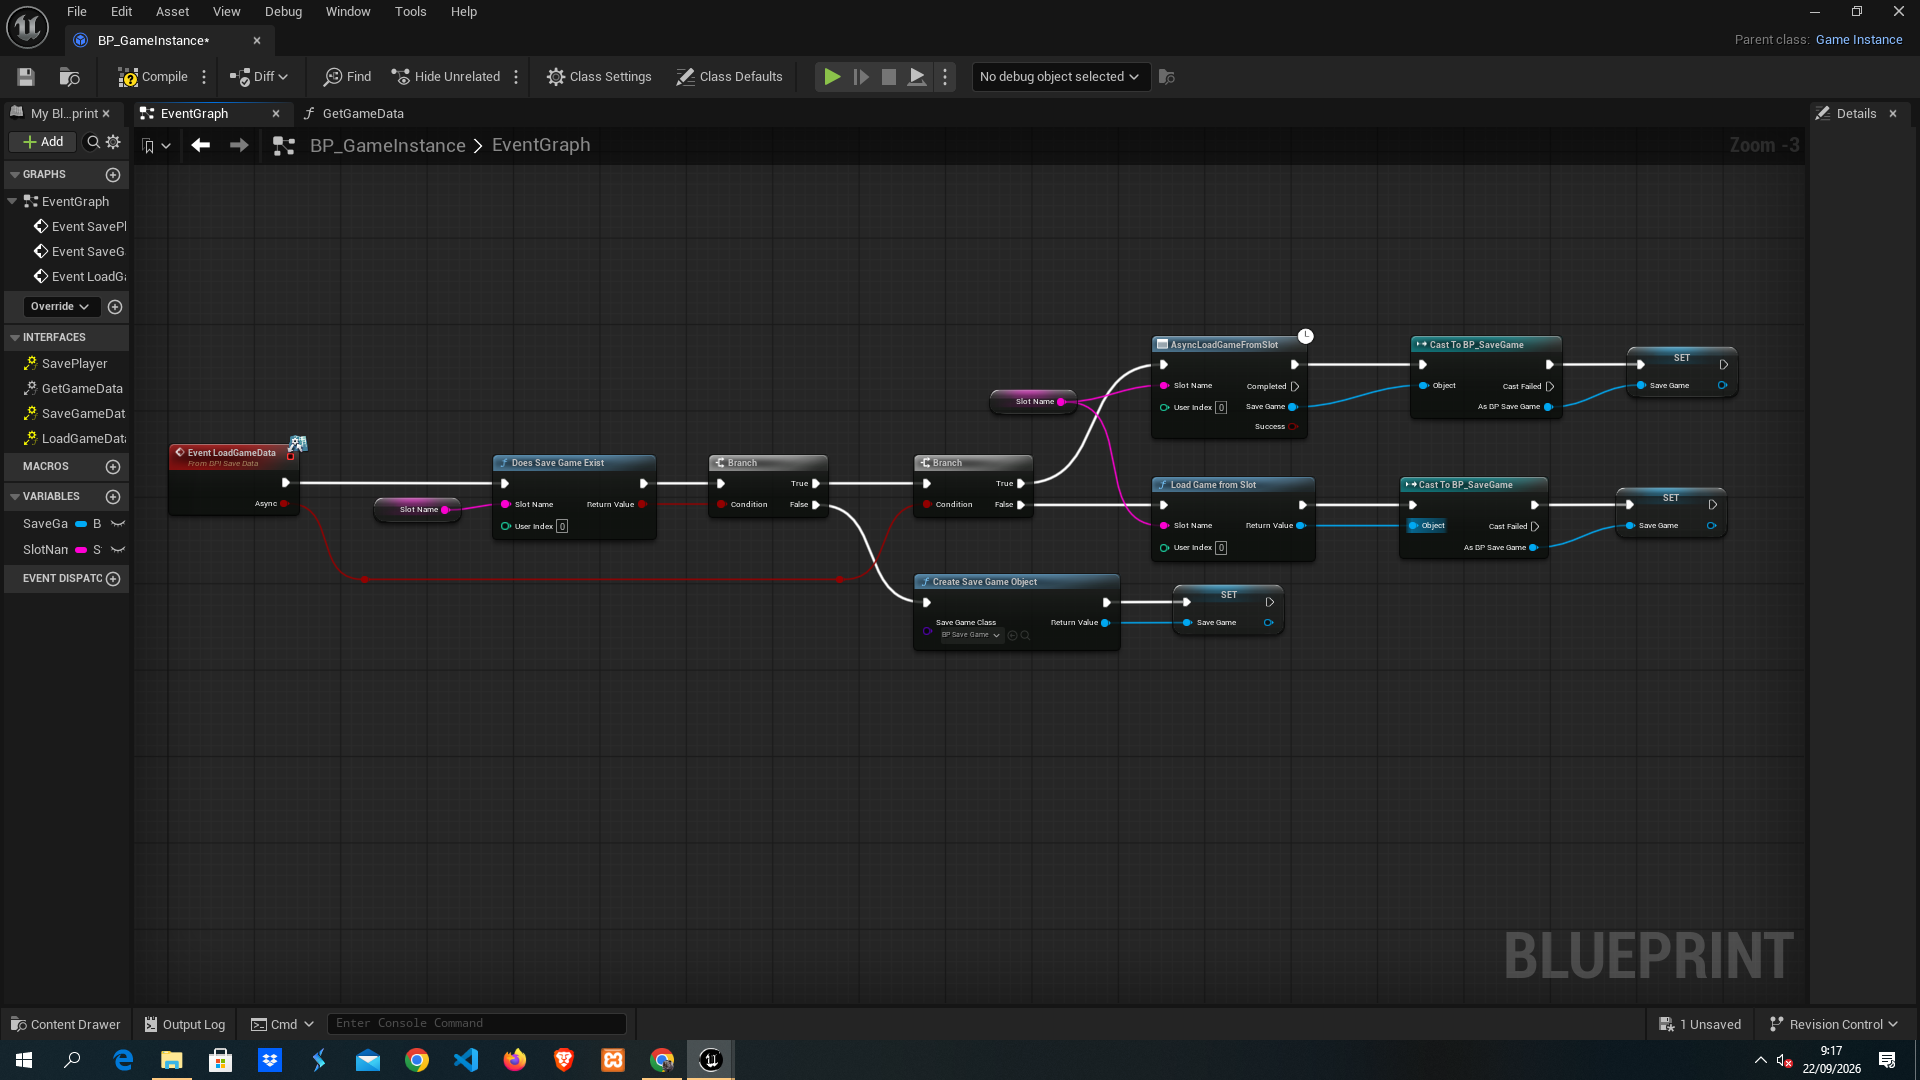
\includegraphics[width=0.8\textwidth]{resource/Dokumentasi/24.png}
  \caption{Navigasi ke Event Graph dan Pemilihan Komponen Box}
  \label{fig:select-box-component-graph}
\end{figure}

\par Berdasarkan Gambar \ref{fig:select-box-component-graph}, saya beralih dari tab \textit{Viewport} menuju ke lembar kerja \textit{Event Graph} pada editor \texttt{BP\_Collision}. Saya memastikan komponen \texttt{Box} tetap dalam kondisi terseleksi aktif pada panel \textit{Components} di sisi kiri atas. Hal ini bertujuan agar menu konteks klik kanan pada kanvas \textit{Event Graph} secara otomatis menampilkan daftar fungsi kejadian tabrakan yang secara spesifik dimiliki oleh komponen kotak tabrakan tersebut.

\begin{figure}[H]
  \centering
  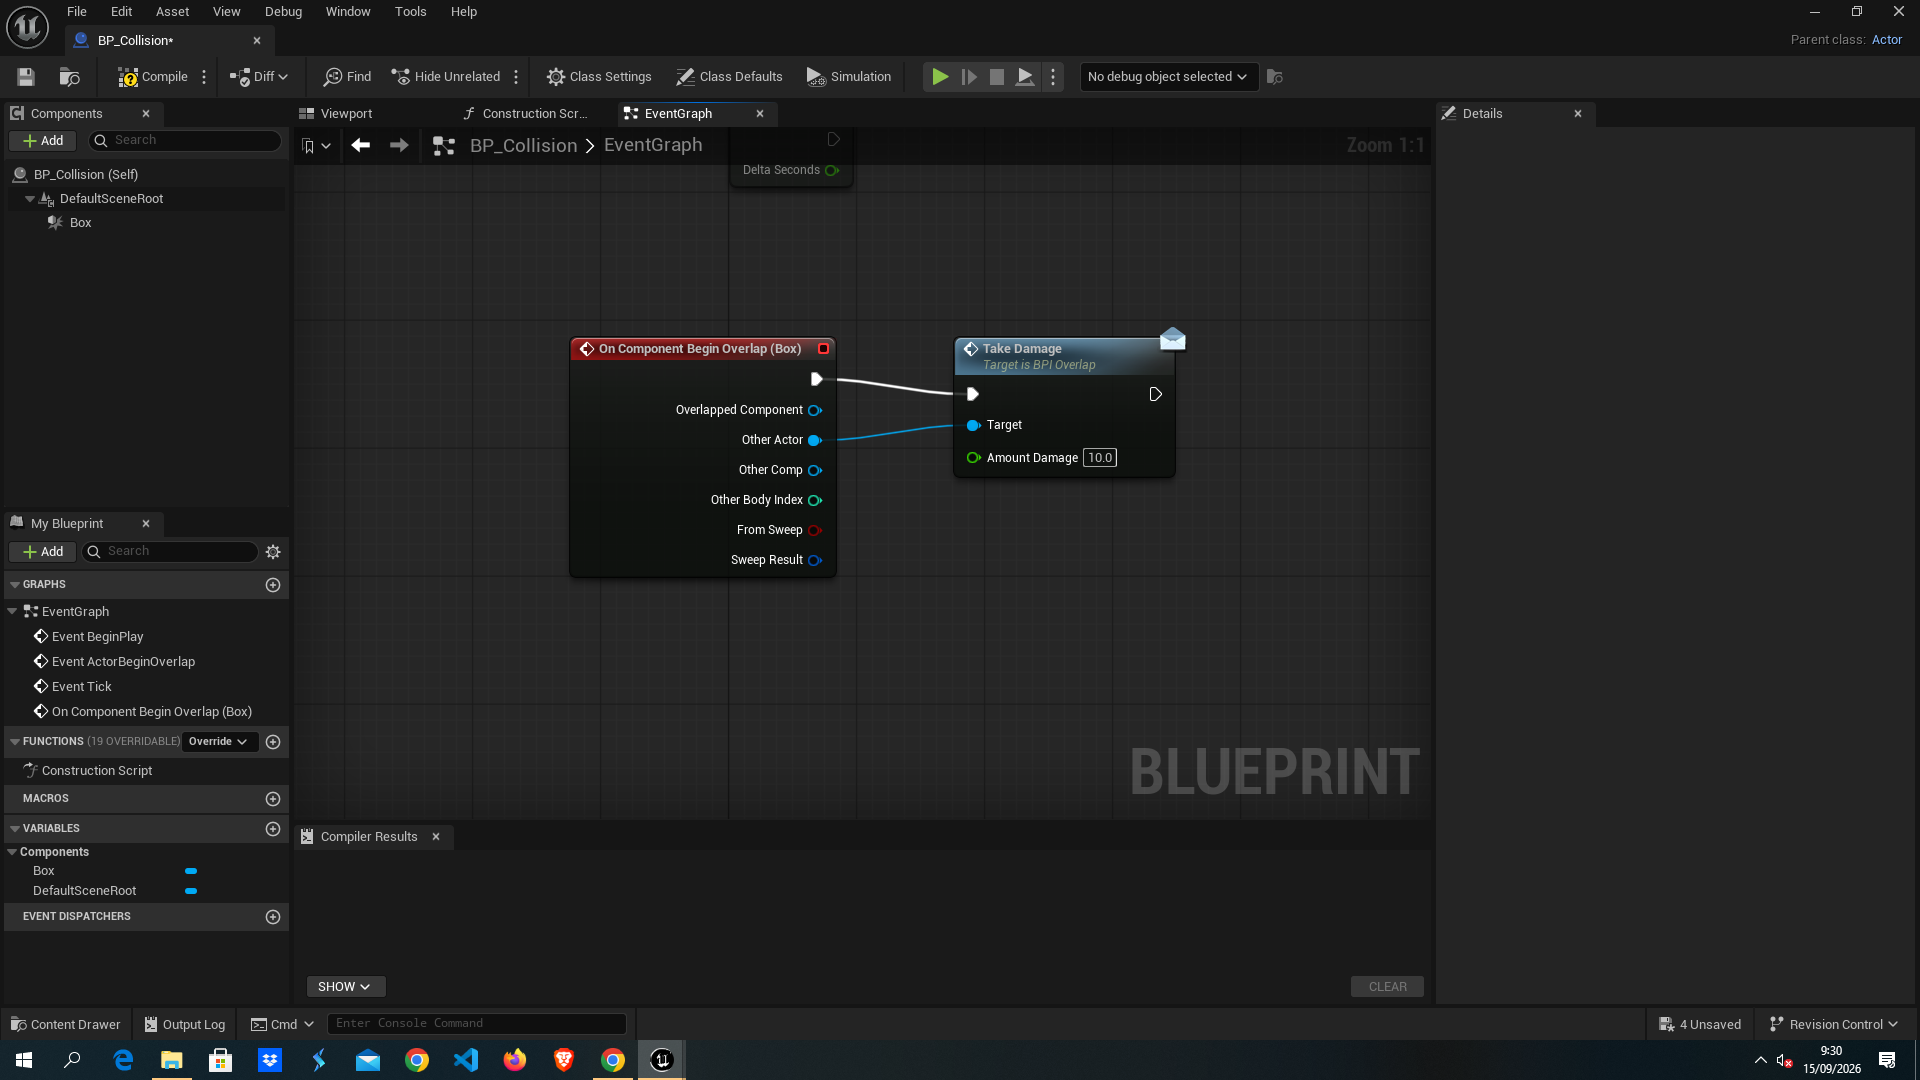
\includegraphics[width=0.8\textwidth]{resource/Dokumentasi/25.png}
  \caption{Penambahan Event On Component Begin Overlap (Box)}
  \label{fig:add-on-begin-overlap-event}
\end{figure}

\par Pada Gambar \ref{fig:add-on-begin-overlap-event}, saya mengeklik kanan pada kanvas kerja dan memilih menu \textit{Add Event for Box > Add On Component Begin Overlap}. Node kejadian \texttt{On Component Begin Overlap (Box)} ini bertindak sebagai sensor pemicu utama yang akan langsung mengeksekusi alur perintah logika seketika ada batas fisik dari aktor luar yang mulai memasuki volume pembatas dari kotak tabrakan \texttt{Box}.

\begin{figure}[H]
  \centering
  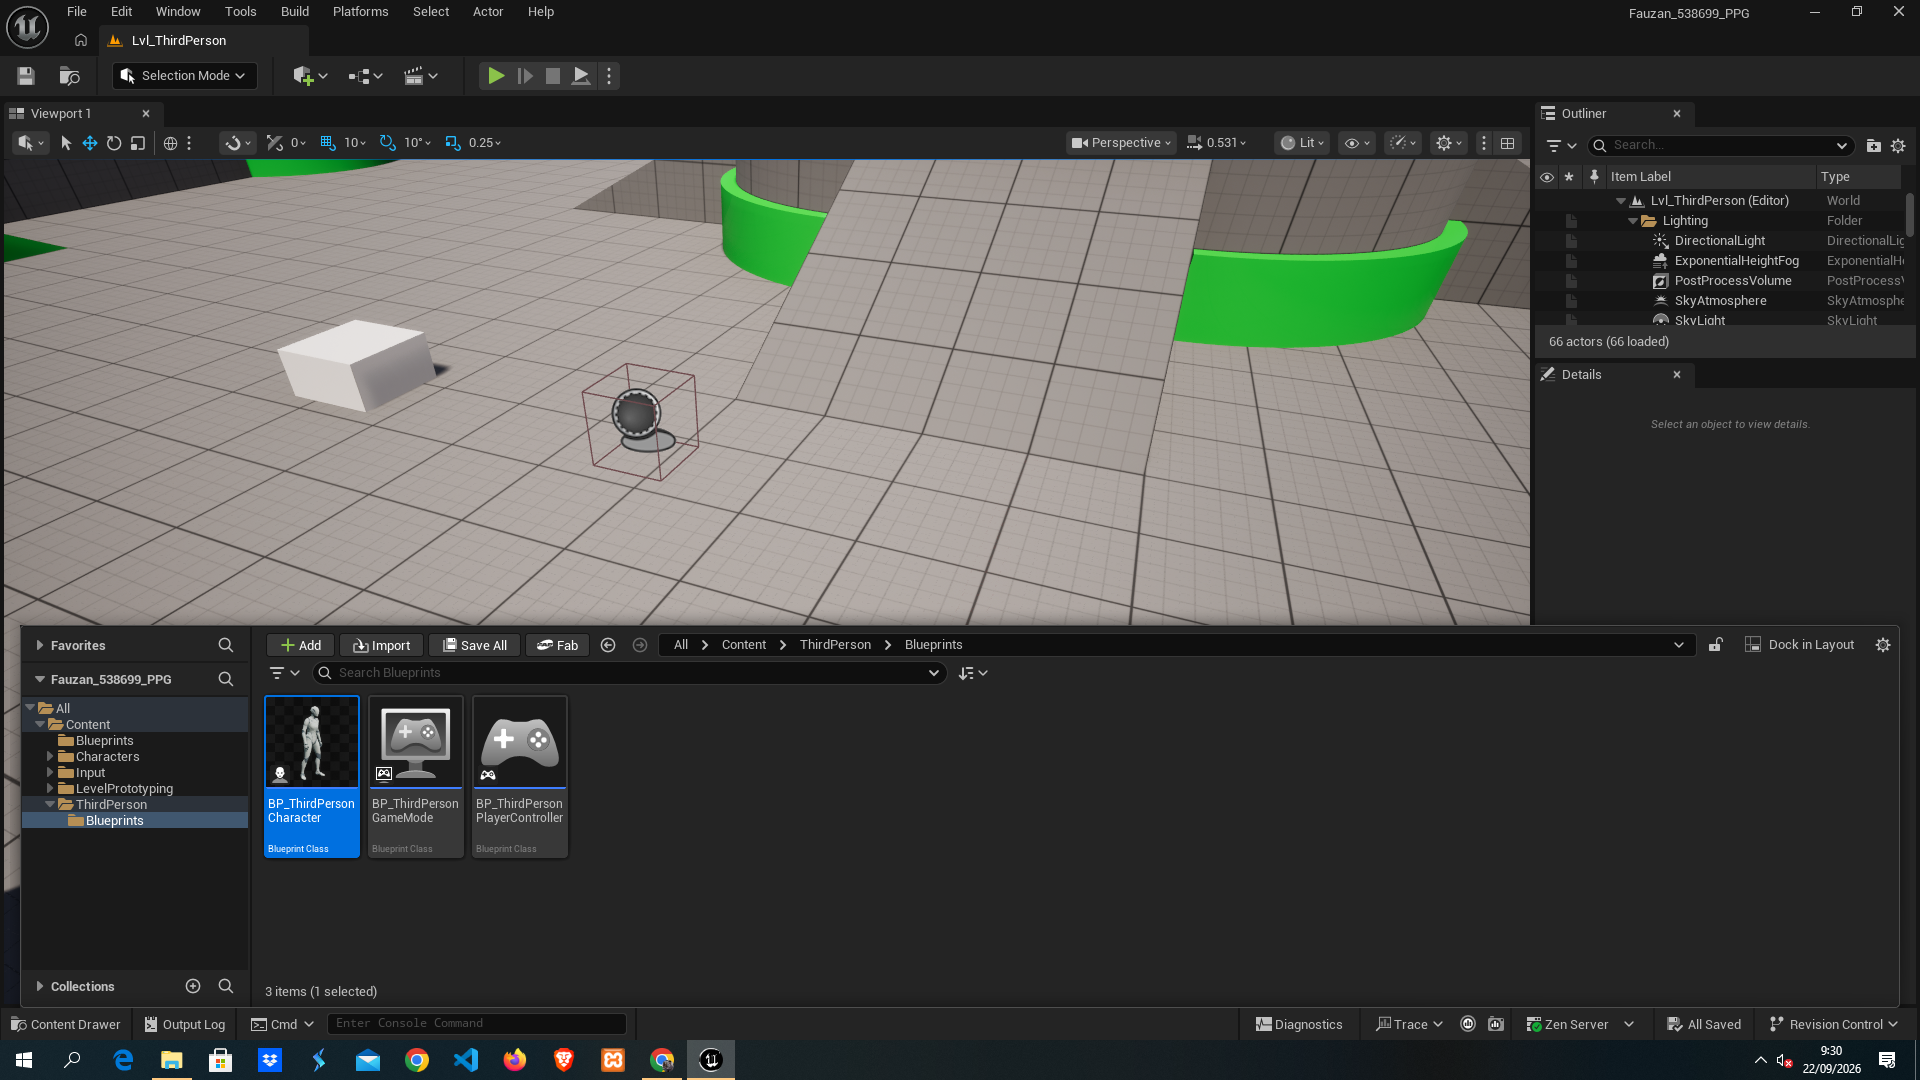
\includegraphics[width=0.8\textwidth]{resource/Dokumentasi/26.png}
  \caption{Pemanggilan Pesan Interface TakeDamage via Pin Other Actor}
  \label{fig:call-takedamage-message}
\end{figure}

\par Melanjutkan perancangan alur interaksi tabrakan, Gambar \ref{fig:call-takedamage-message} memperlihatkan integrasi pesan antarmuka pada node tabrakan. Saya menarik kabel dari pin referensi \texttt{Other Actor} milik node overlap, kemudian mencari dan memanggil fungsi antarmuka \texttt{TakeDamage (Message)}. Karena menggunakan mekanisme pesan antarmuka (\textit{Interface Message}), pemanggilan ini bersifat sangat aman dan bebas galat: apabila aktor yang menabrak kotak mengimplementasikan kontrak antarmuka \texttt{BPI\_Overlap}, perintah kerusakan akan diproses secara instan; sebaliknya jika aktor yang menabrak tidak mengadopsi antarmuka tersebut, sistem Unreal Engine akan mengabaikannya secara otomatis tanpa menimbulkan kegagalan program (\textit{crash}).

\begin{figure}[H]
  \centering
  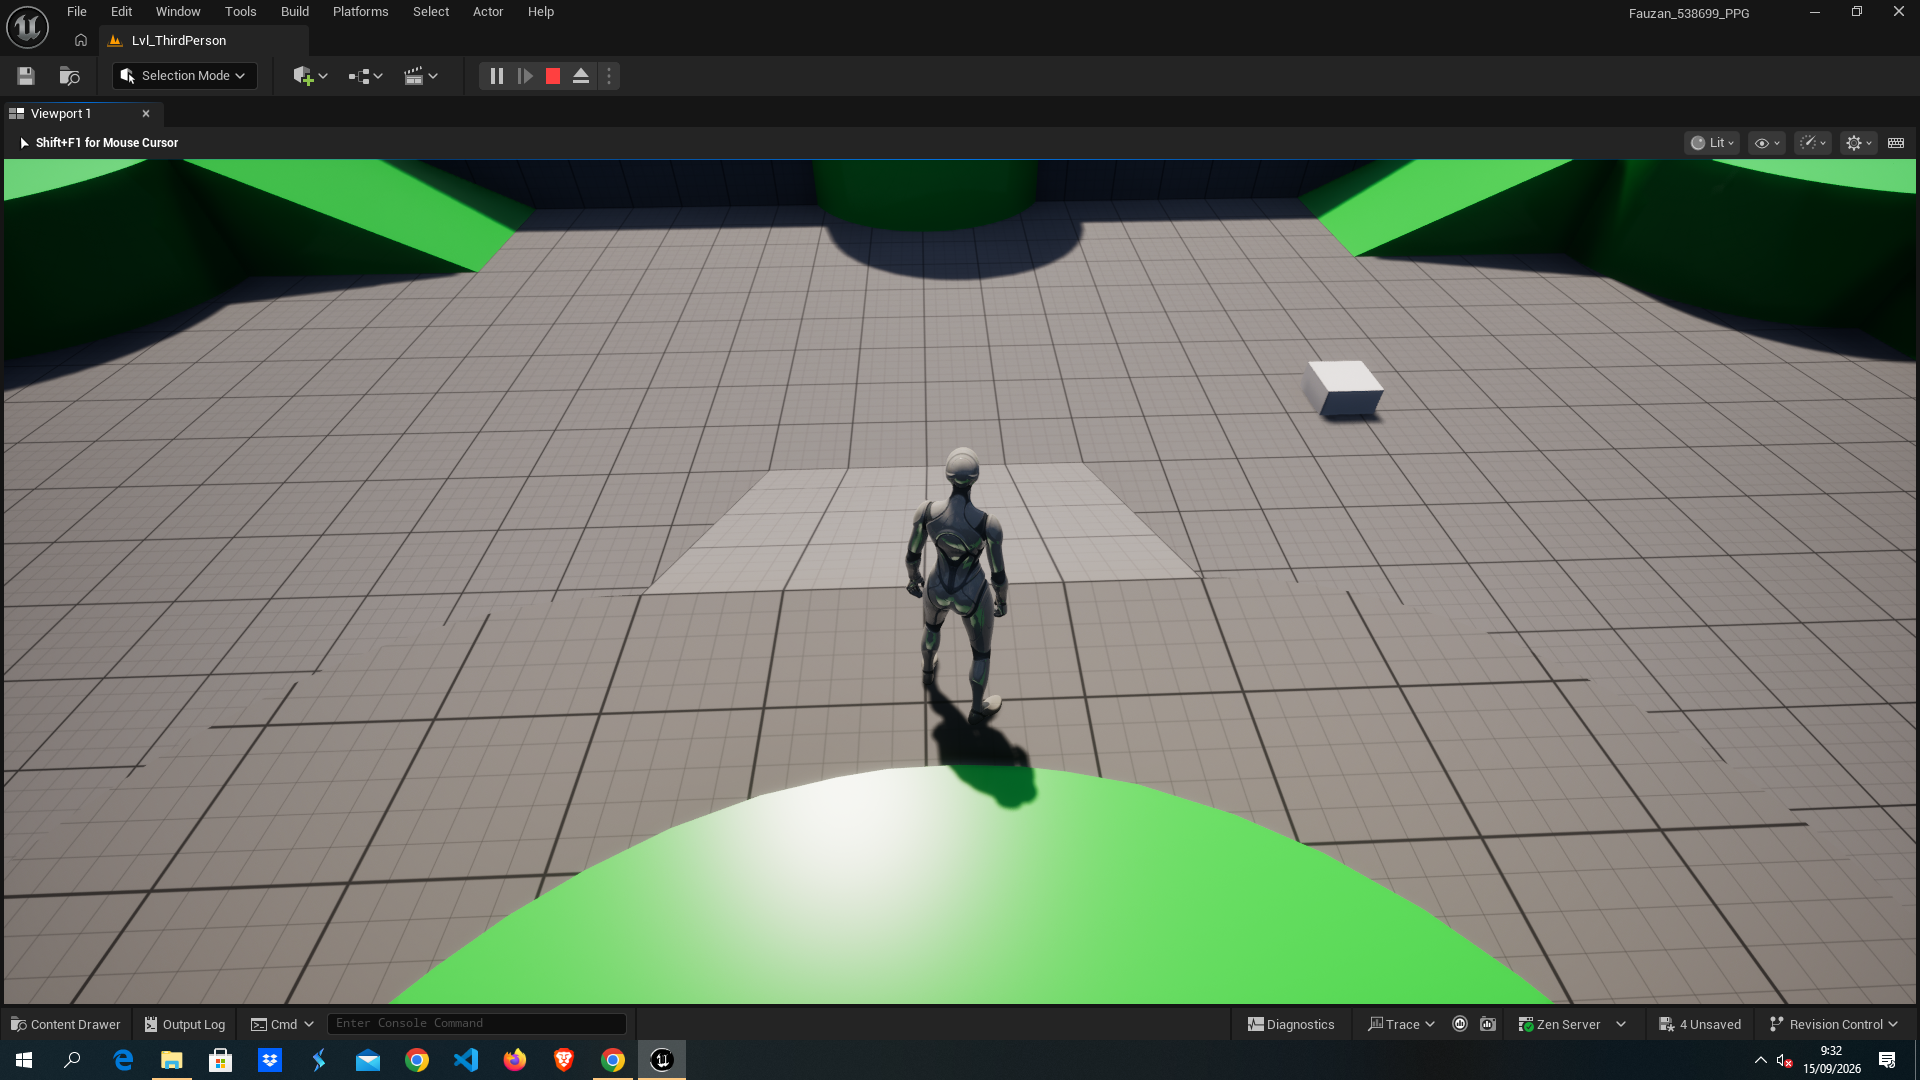
\includegraphics[width=0.8\textwidth]{resource/Dokumentasi/27.png}
  \caption{Penetapan Nilai Literal Kerusakan pada Parameter AmountDamage}
  \label{fig:set-literal-damage-value}
\end{figure}

\par Berdasarkan Gambar \ref{fig:set-literal-damage-value}, saya menetapkan nilai numerik konstan sebesar 20.0 secara langsung pada pin masukan \texttt{AmountDamage} di node \texttt{TakeDamage (Message)}. Nilai konstan ini digunakan sebagai pengujian tahap awal untuk memastikan bahwa seluruh rantai komunikasi tabrakan dan antarmuka dapat berjalan normal dalam mengurangi nilai kesehatan karakter sebelum sistem parameterisasi variabel diterapkan.

\begin{figure}[H]
  \centering
  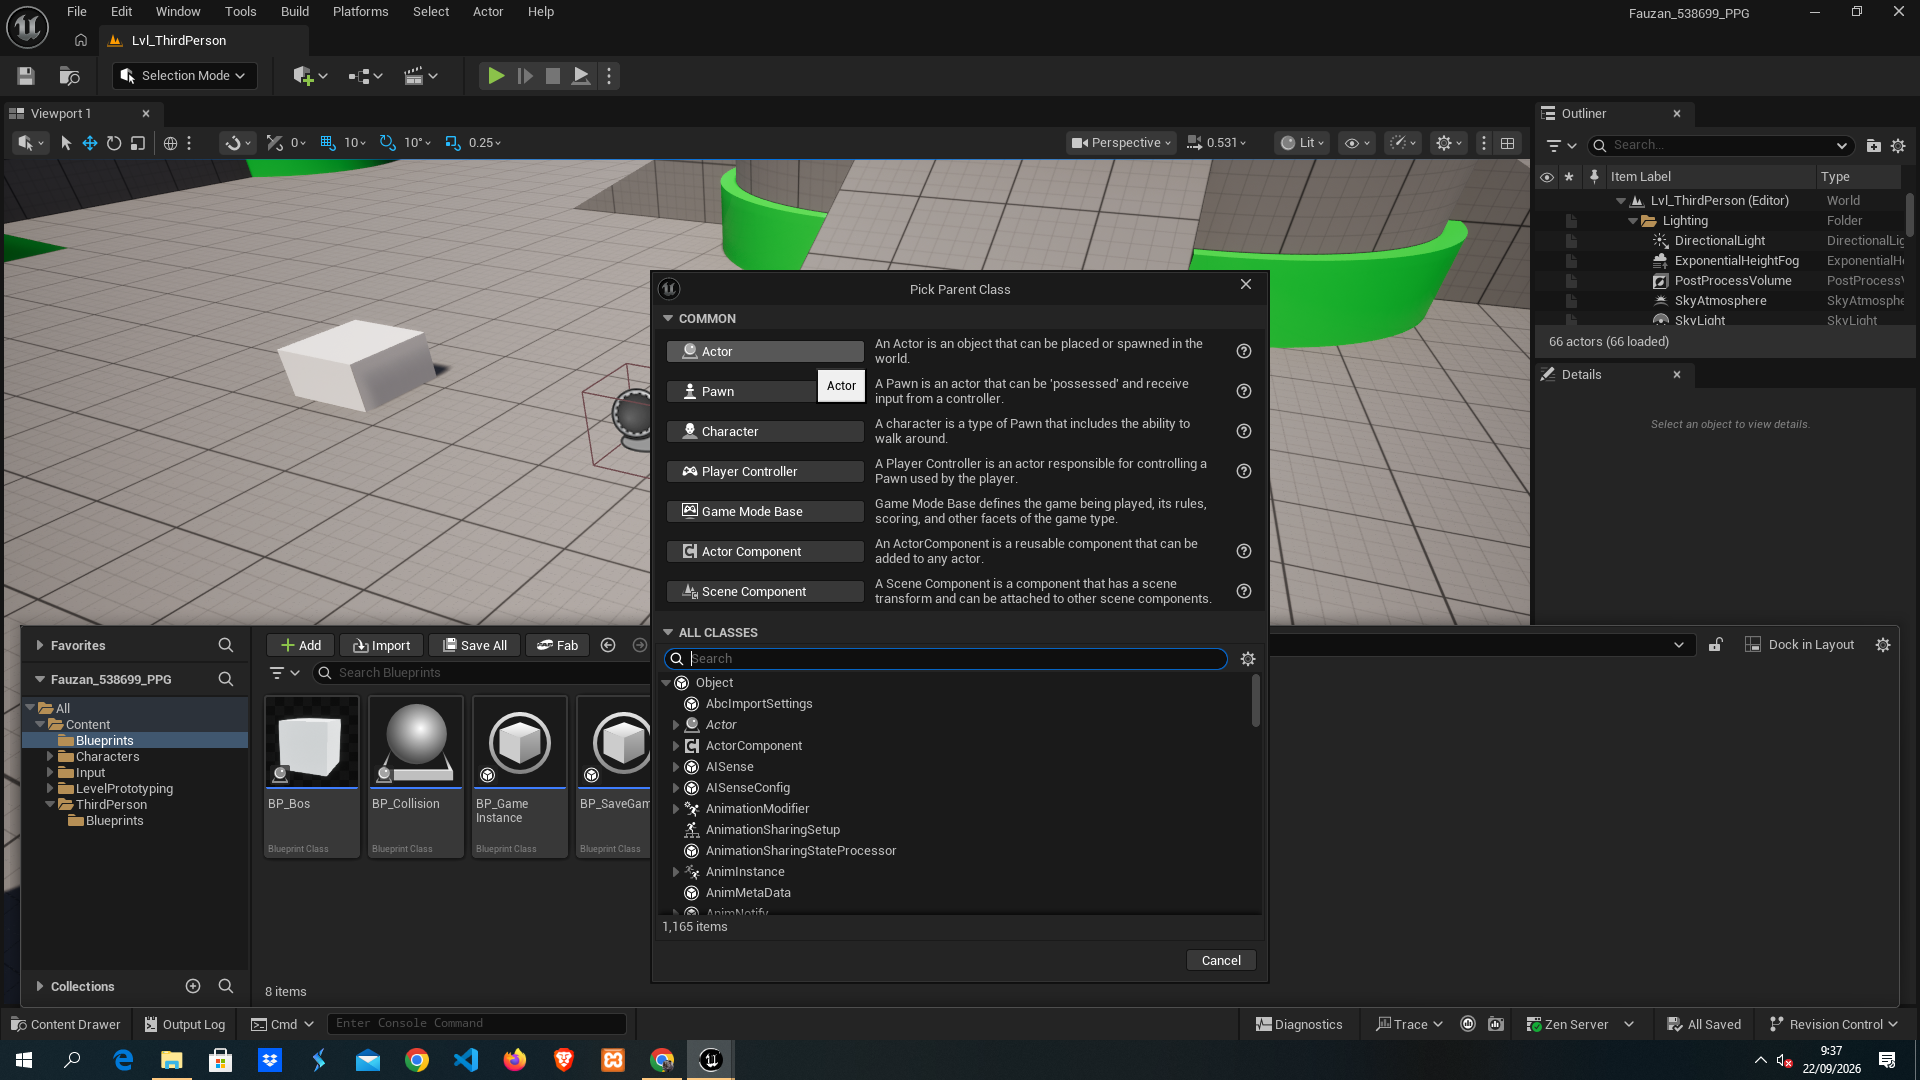
\includegraphics[width=0.8\textwidth]{resource/Dokumentasi/28.png}
  \caption{Penempatan Aset BP\_Collision ke Level Editor}
  \label{fig:drag-bp-collision-to-level}
\end{figure}

\par Pada Gambar \ref{fig:drag-bp-collision-to-level}, setelah melakukan kompilasi terhadap \texttt{BP\_Collision}, saya menyeret (\textit{drag-and-drop}) aset tersebut langsung dari Content Drawer ke dalam jendela level editor kerja. Instansiasi objek aktor ini ditempatkan tepat di atas permukaan lantai arena uji coba permainan agar dapat dijangkau dan dilintasi secara langsung oleh karakter pemain saat bergerak.

\begin{figure}[H]
  \centering
  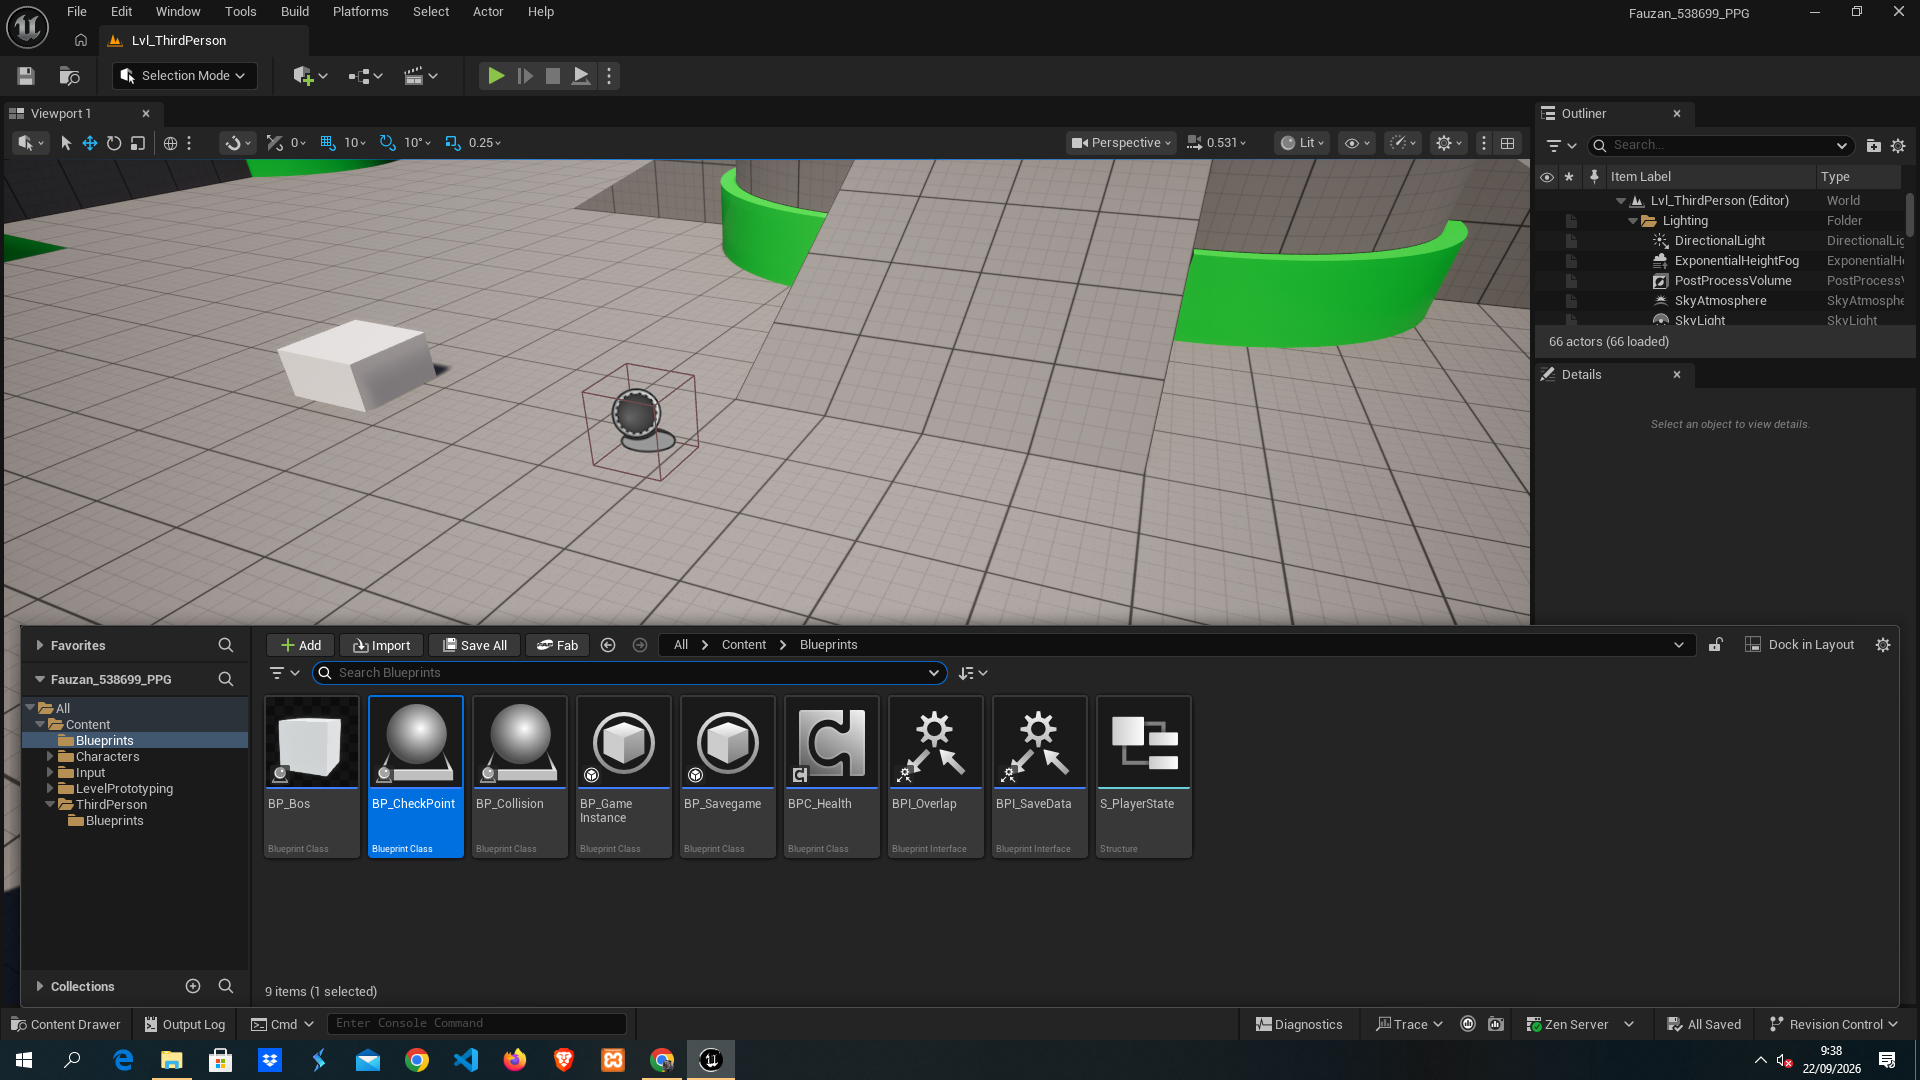
\includegraphics[width=0.8\textwidth]{resource/Dokumentasi/29.png}
  \caption{Pengaturan Transformasi dan Posisi Spasial BP\_Collision di Level}
  \label{fig:adjust-transform-bp-collision}
\end{figure}

\par Langkah berlanjut dengan menyesuaikan koordinat posisi aktor, seperti tampak pada Gambar \ref{fig:adjust-transform-bp-collision}. Menggunakan \textit{gizmo} translasi tiga sumbu di viewport level, saya menyetel ketinggian dan posisi spasial aktor \texttt{BP\_Collision} agar sejajar dengan jalur pergerakan karakter pemain. Penempatan yang presisi ini sangat krusial untuk memastikan bahwa volume tabrakan berada pada elevasi yang pas dan dapat menyentuh kapsul tabrakan karakter saat simulasi dijalankan.

\begin{figure}[H]
  \centering
  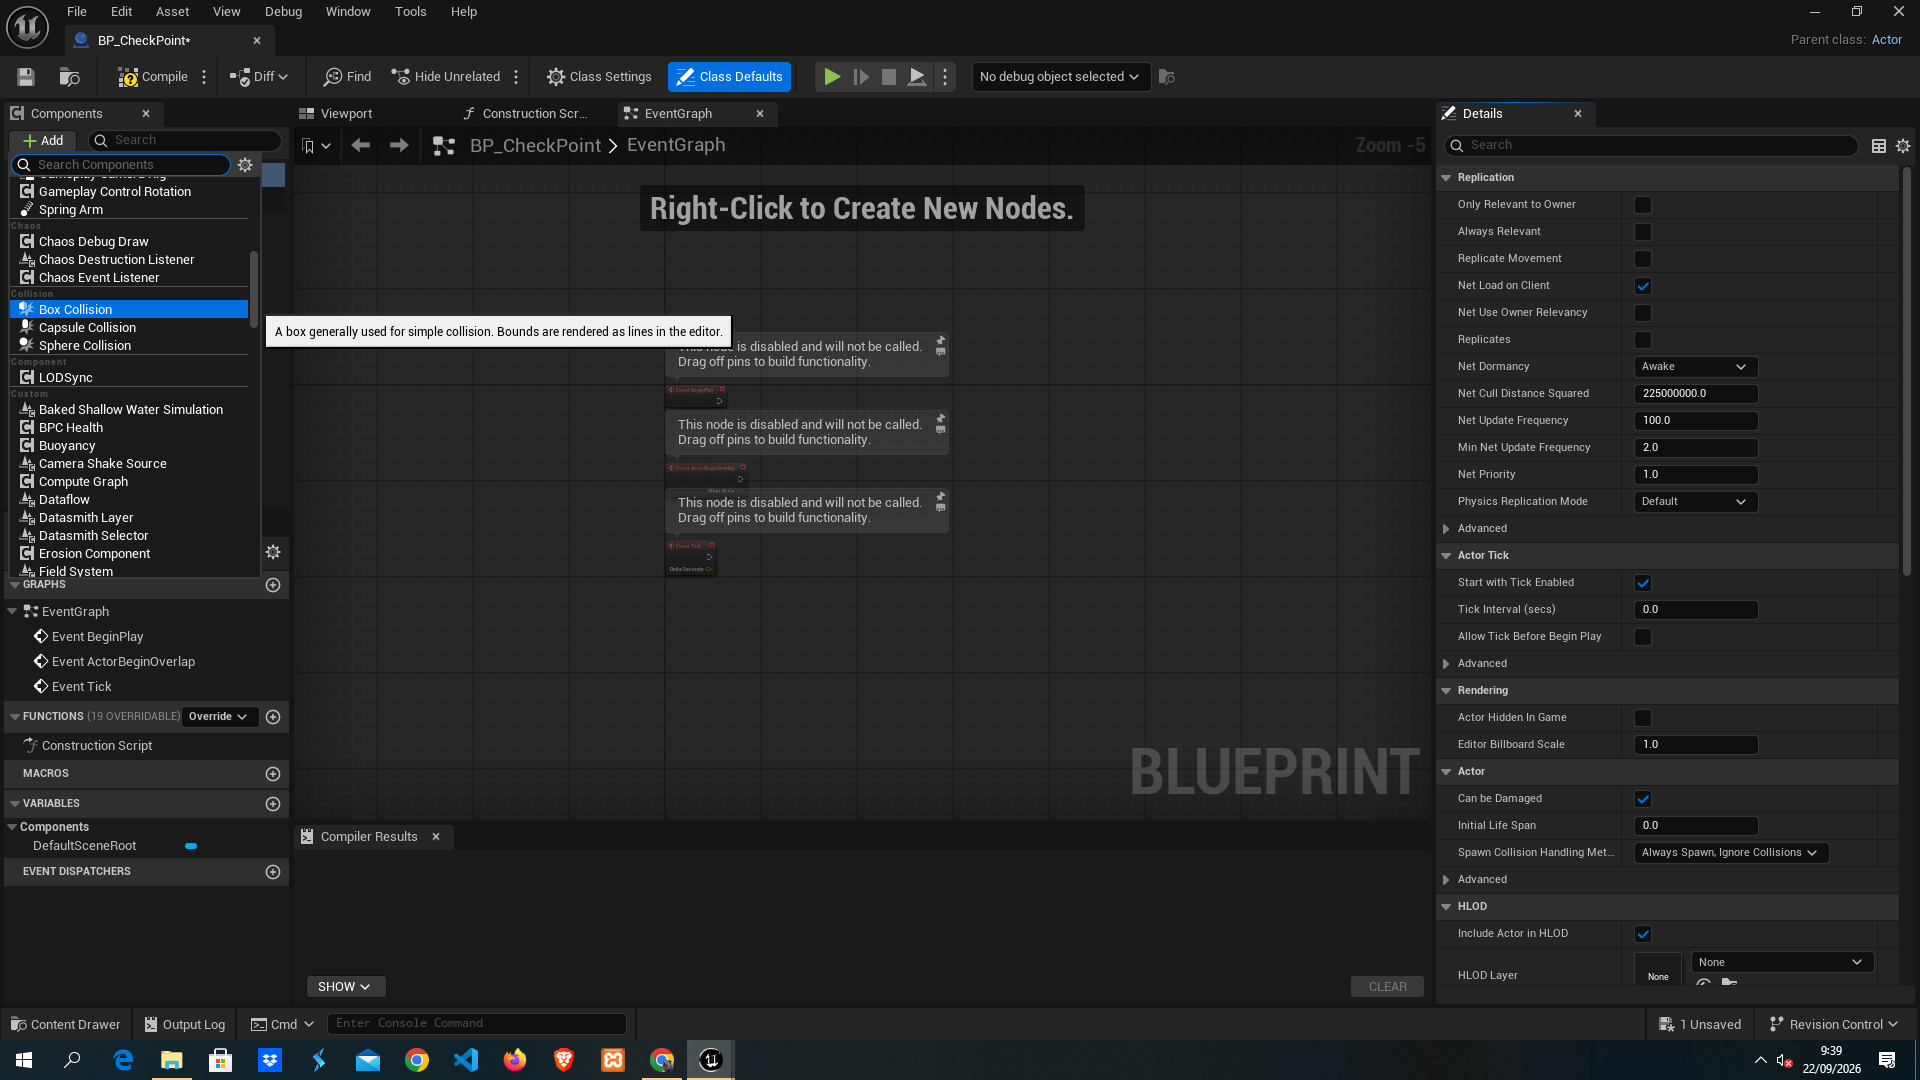
\includegraphics[width=0.8\textwidth]{resource/Dokumentasi/30.png}
  \caption{Seleksi Komponen Box pada Instance BP\_Collision di Level}
  \label{fig:select-box-component-details}
\end{figure}

\par Berdasarkan Gambar \ref{fig:select-box-component-details}, saya memilih komponen anak \texttt{Box} pada aktor \texttt{BP\_Collision} melalui panel \textit{Details} di jendela editor level. Tindakan seleksi spesifik ini membuka seluruh daftar parameter properti rendering dan perilaku fisik dari komponen kotak tabrakan tersebut, memungkinkan penyesuaian properti tampilan secara khusus saat permainan berlangsung.

\begin{figure}[H]
  \centering
  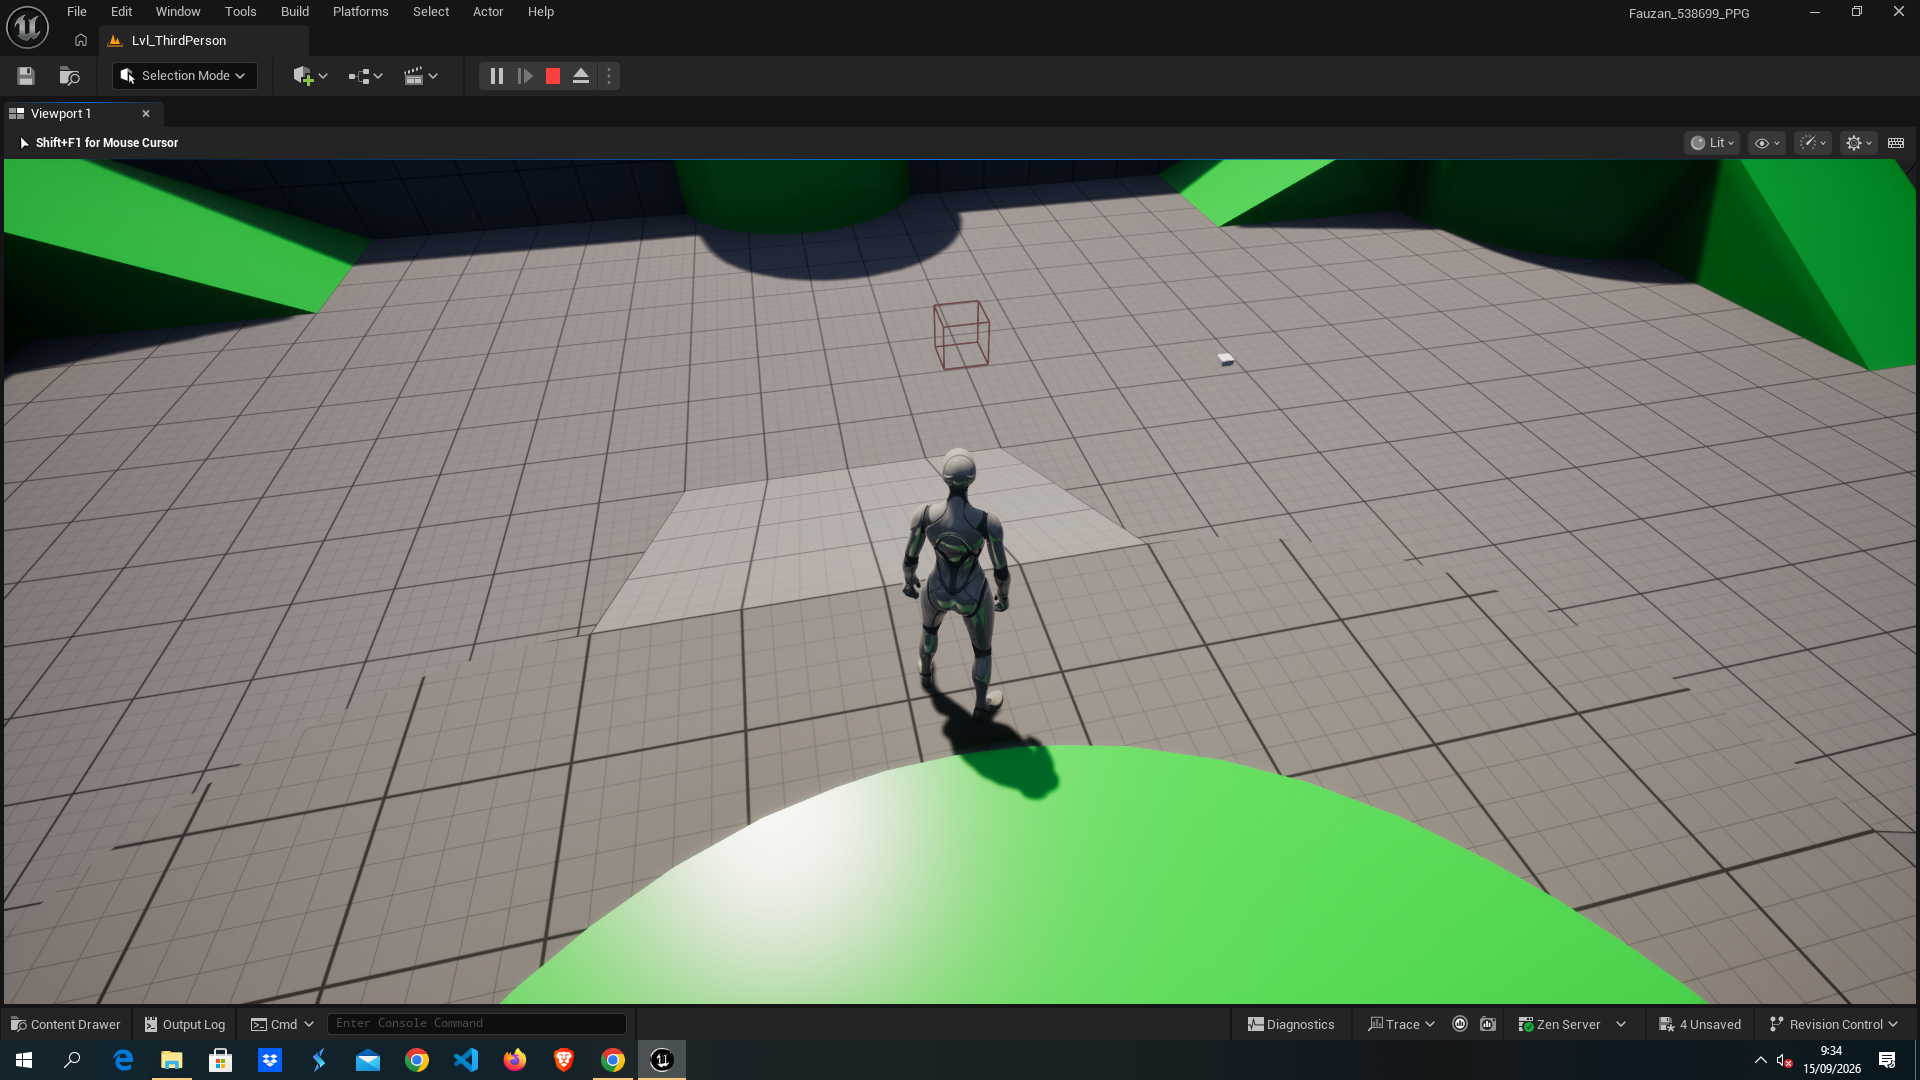
\includegraphics[width=0.8\textwidth]{resource/Dokumentasi/31.png}
  \caption{Menghilangkan Centang Opsi Hidden in Game pada Komponen Box}
  \label{fig:uncheck-hidden-in-game}
\end{figure}

\par Pada Gambar \ref{fig:uncheck-hidden-in-game}, saya menavigasi ke bagian \textit{Rendering} pada panel \textit{Details} komponen \texttt{Box}, lalu menghapus tanda centang pada opsi \texttt{Hidden in Game}. Secara baku, Unreal Engine menyembunyikan seluruh komponen volume tabrakan saat permainan dijalankan demi efisiensi visual; namun dengan mematikan opsi ini, kerangka kawat (\textit{wireframe}) berwarna kuning dari kotak tabrakan akan tetap diproyeksikan secara visual selama simulasi \textit{Play-in-Editor} berlangsung, sangat membantu proses verifikasi dan \textit{debugging} visual.

\begin{figure}[H]
  \centering
  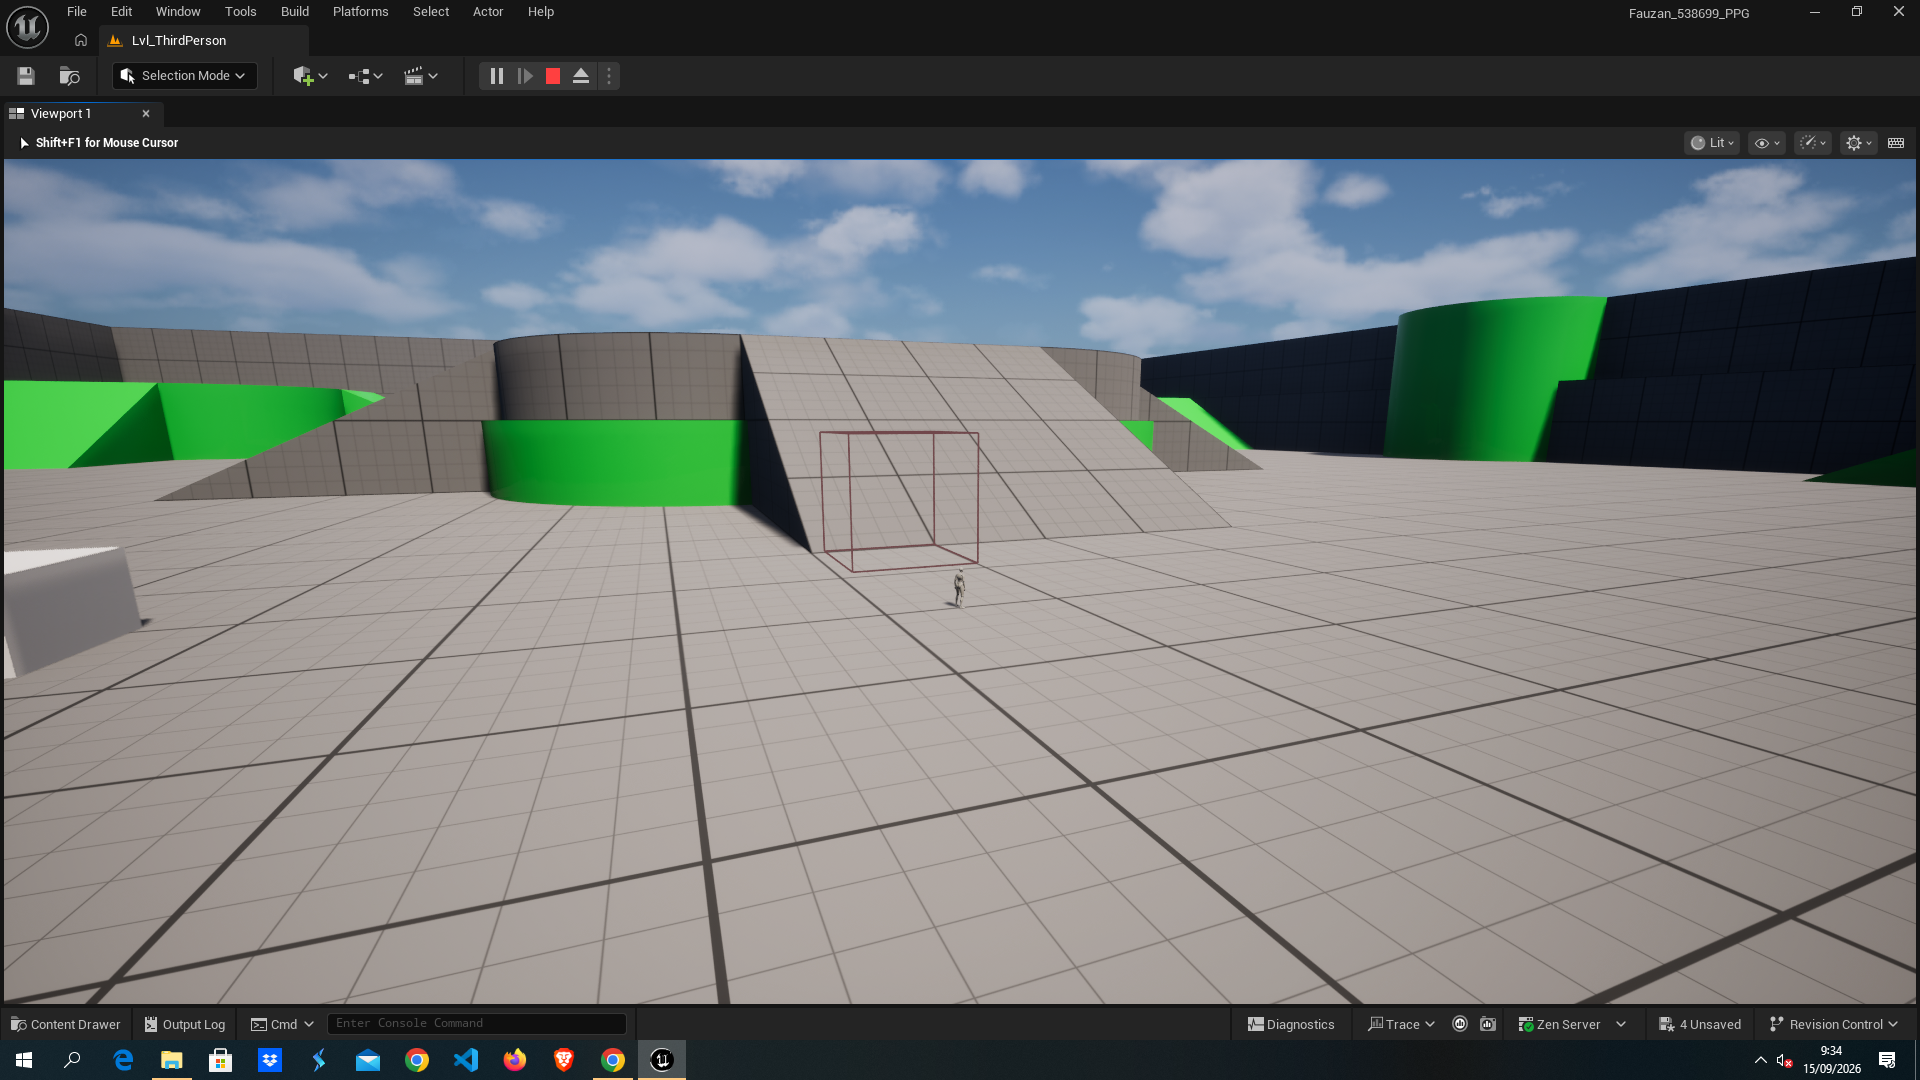
\includegraphics[width=0.8\textwidth]{resource/Dokumentasi/32.png}
  \caption{Kompilasi dan Penyimpanan Akhir Blueprint BP\_Collision}
  \label{fig:compile-save-bp-collision}
\end{figure}

\par Berdasarkan Gambar \ref{fig:compile-save-bp-collision}, saya mengompilasi dan menyimpan \textit{Blueprint} \texttt{BP\_Collision}. Tanda centang hijau pada tombol \textit{Compile} menandakan bahwa seluruh konfigurasi komponen dan grafik logika telah bebas dari galat sintaks maupun referensi, memastikan aktor perangkap tabrakan siap menerima konfigurasi variabel dinamis pada tahap selanjutnya.

\subsection{Konfigurasi Instance Editable Variable dan Validasi Simulasi Interaktif}

\par Untuk meningkatkan fleksibilitas dalam proses perancangan level (\textit{level design}), besaran nilai kerusakan yang diberikan oleh perangkap tabrakan perlu diatur secara dinamis per instansiasi objek di dunia permainan tanpa harus membuka atau memodifikasi grafik logika dasar \textit{Blueprint}. Pada subbab ini, saya mengonfigurasi variabel \textit{Instance Editable} dan memvalidasi keseluruhan alur interaksi secara komprehensif melalui simulasi interaktif \textit{Play-in-Editor}.

\begin{figure}[H]
  \centering
  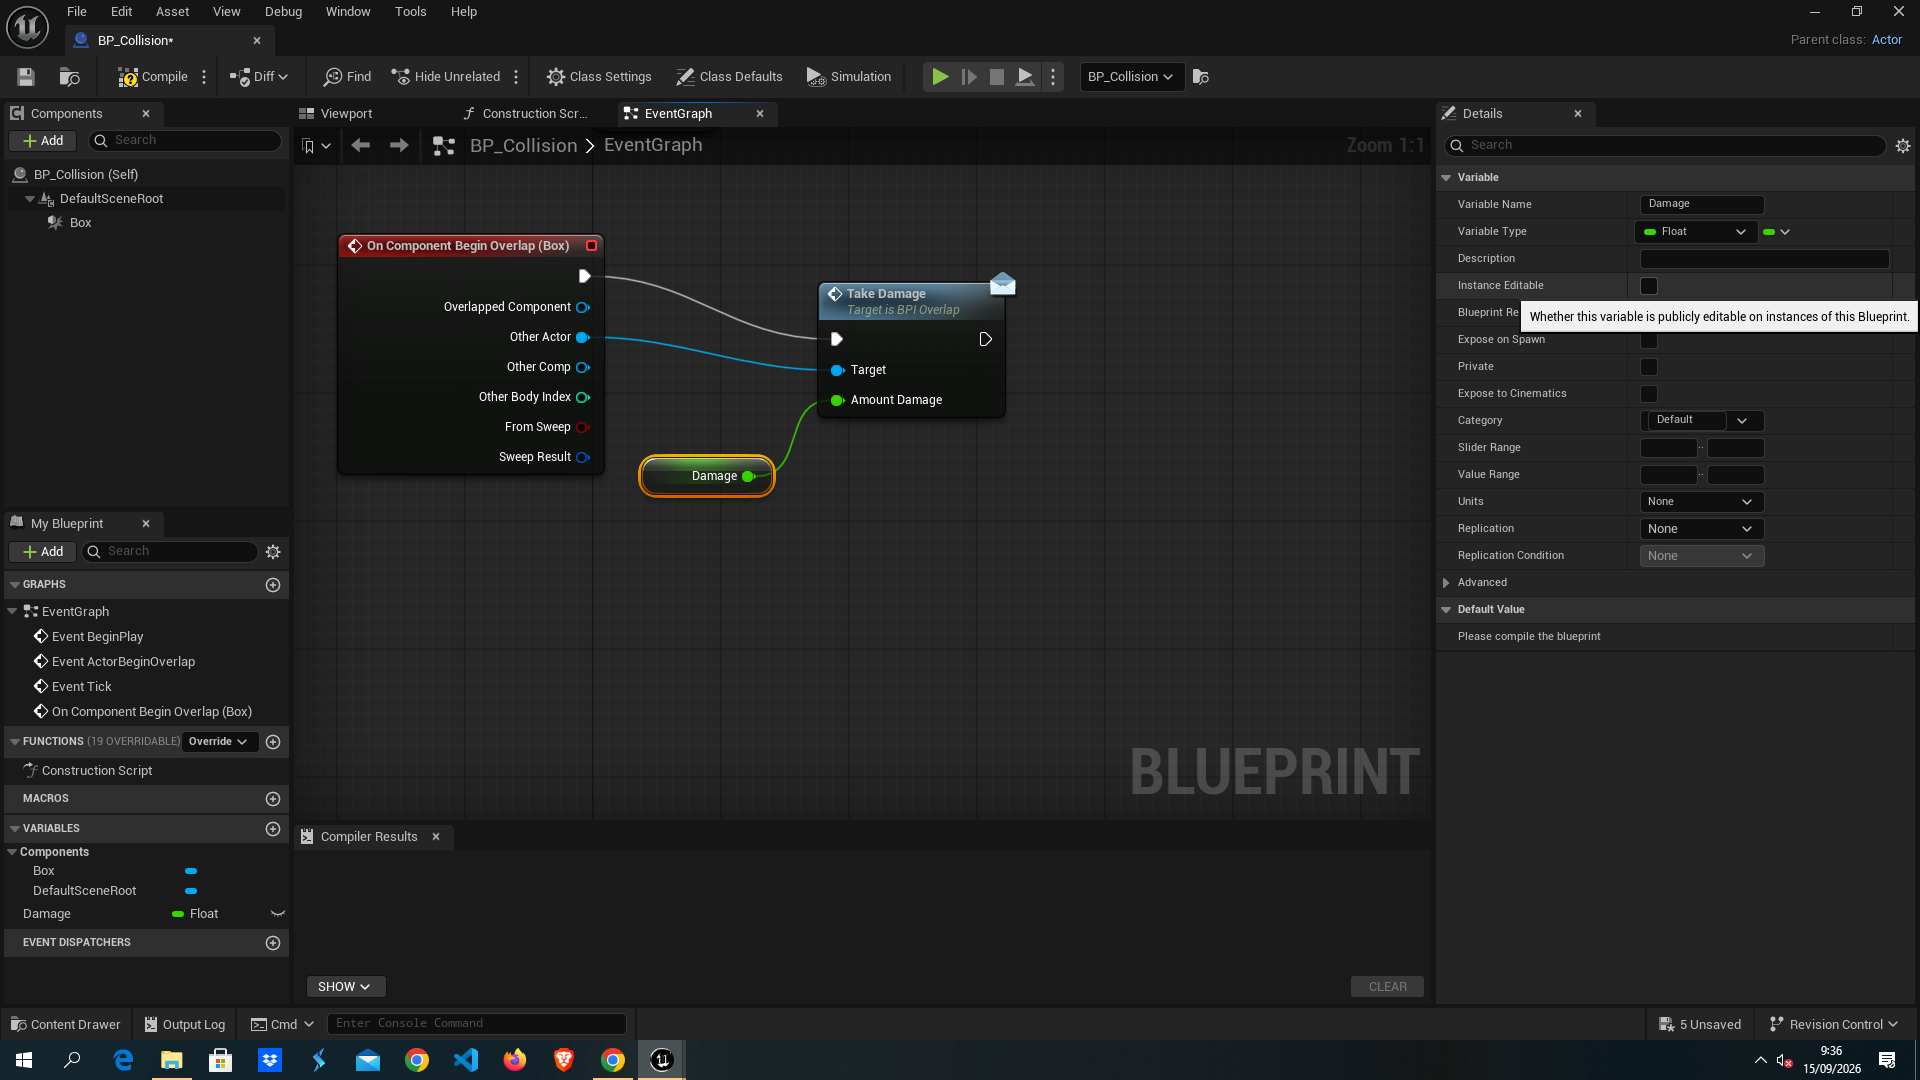
\includegraphics[width=0.8\textwidth]{resource/Dokumentasi/33.png}
  \caption{Pembuatan Variabel Damage pada BP\_Collision}
  \label{fig:create-var-damage}
\end{figure}

\par Berdasarkan Gambar \ref{fig:create-var-damage}, saya kembali ke editor \texttt{BP\_Collision} untuk mendeklarasikan variabel baru bernama \texttt{Damage} pada panel \textit{My Blueprint}. Saya menetapkan tipe datanya sebagai \textit{Float} dengan kode warna hijau terang. Keberadaan variabel ini dirancang untuk menggantikan nilai konstan literal yang sebelumnya dipasang secara statis pada pemanggilan pesan antarmuka, sehingga memberikan fleksibilitas nilai kerusakan yang adaptif.

\begin{figure}[H]
  \centering
  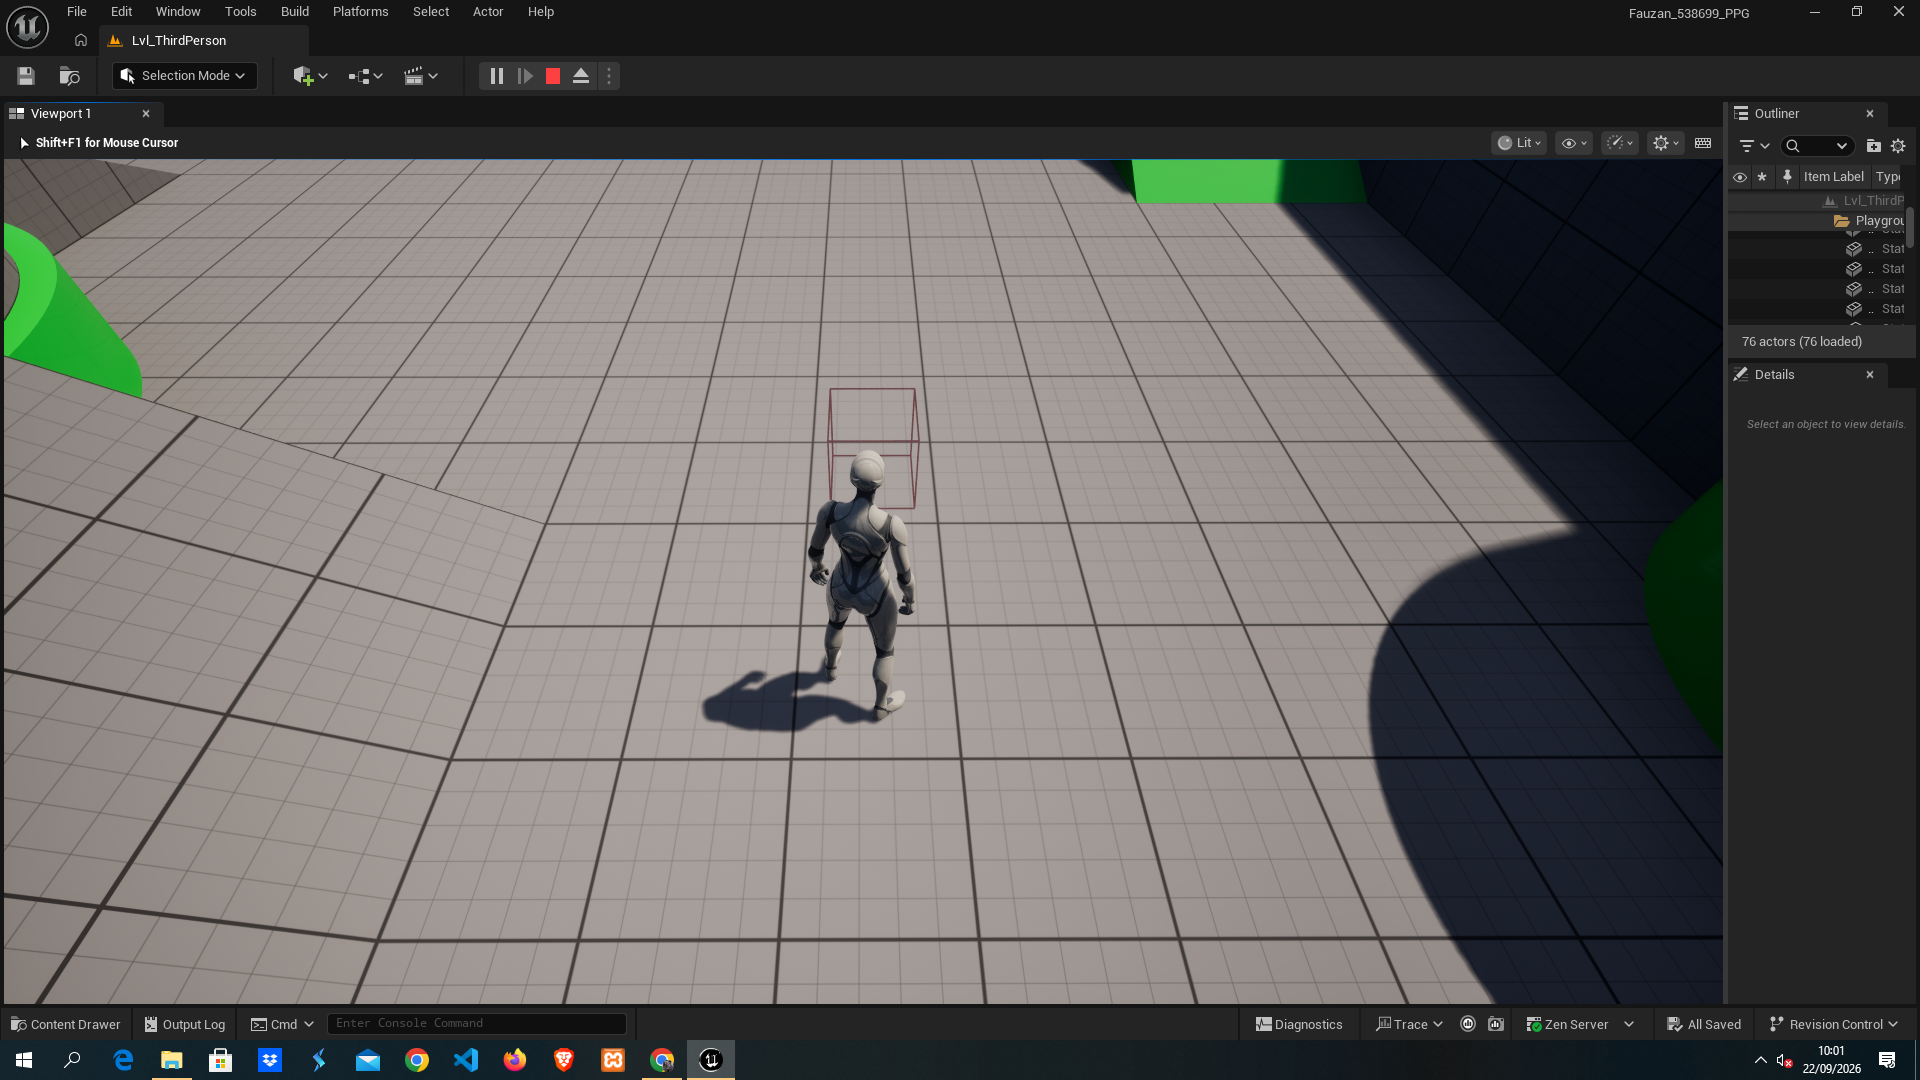
\includegraphics[width=0.8\textwidth]{resource/Dokumentasi/34.png}
  \caption{Pengaktifan Opsi Instance Editable pada Variabel Damage}
  \label{fig:enable-instance-editable}
\end{figure}

\par Pada Gambar \ref{fig:enable-instance-editable}, saya mengaktifkan opsi \textit{Instance Editable} pada variabel \texttt{Damage}. Tindakan ini dilakukan dengan mengeklik ikon mata tertutup di sebelah nama variabel hingga berubah menjadi ikon mata terbuka berwarna hijau pada panel \textit{My Blueprint}, atau dengan mencentang opsi \textit{Instance Editable} pada panel \textit{Details}. Fitur ini mengubah sifat variabel menjadi parameter publik per instans objek di level, memungkinkan setiap instans perangkap tabrakan memiliki nilai kerusakan yang berbeda-beda tanpa saling memengaruhi.

\begin{figure}[H]
  \centering
  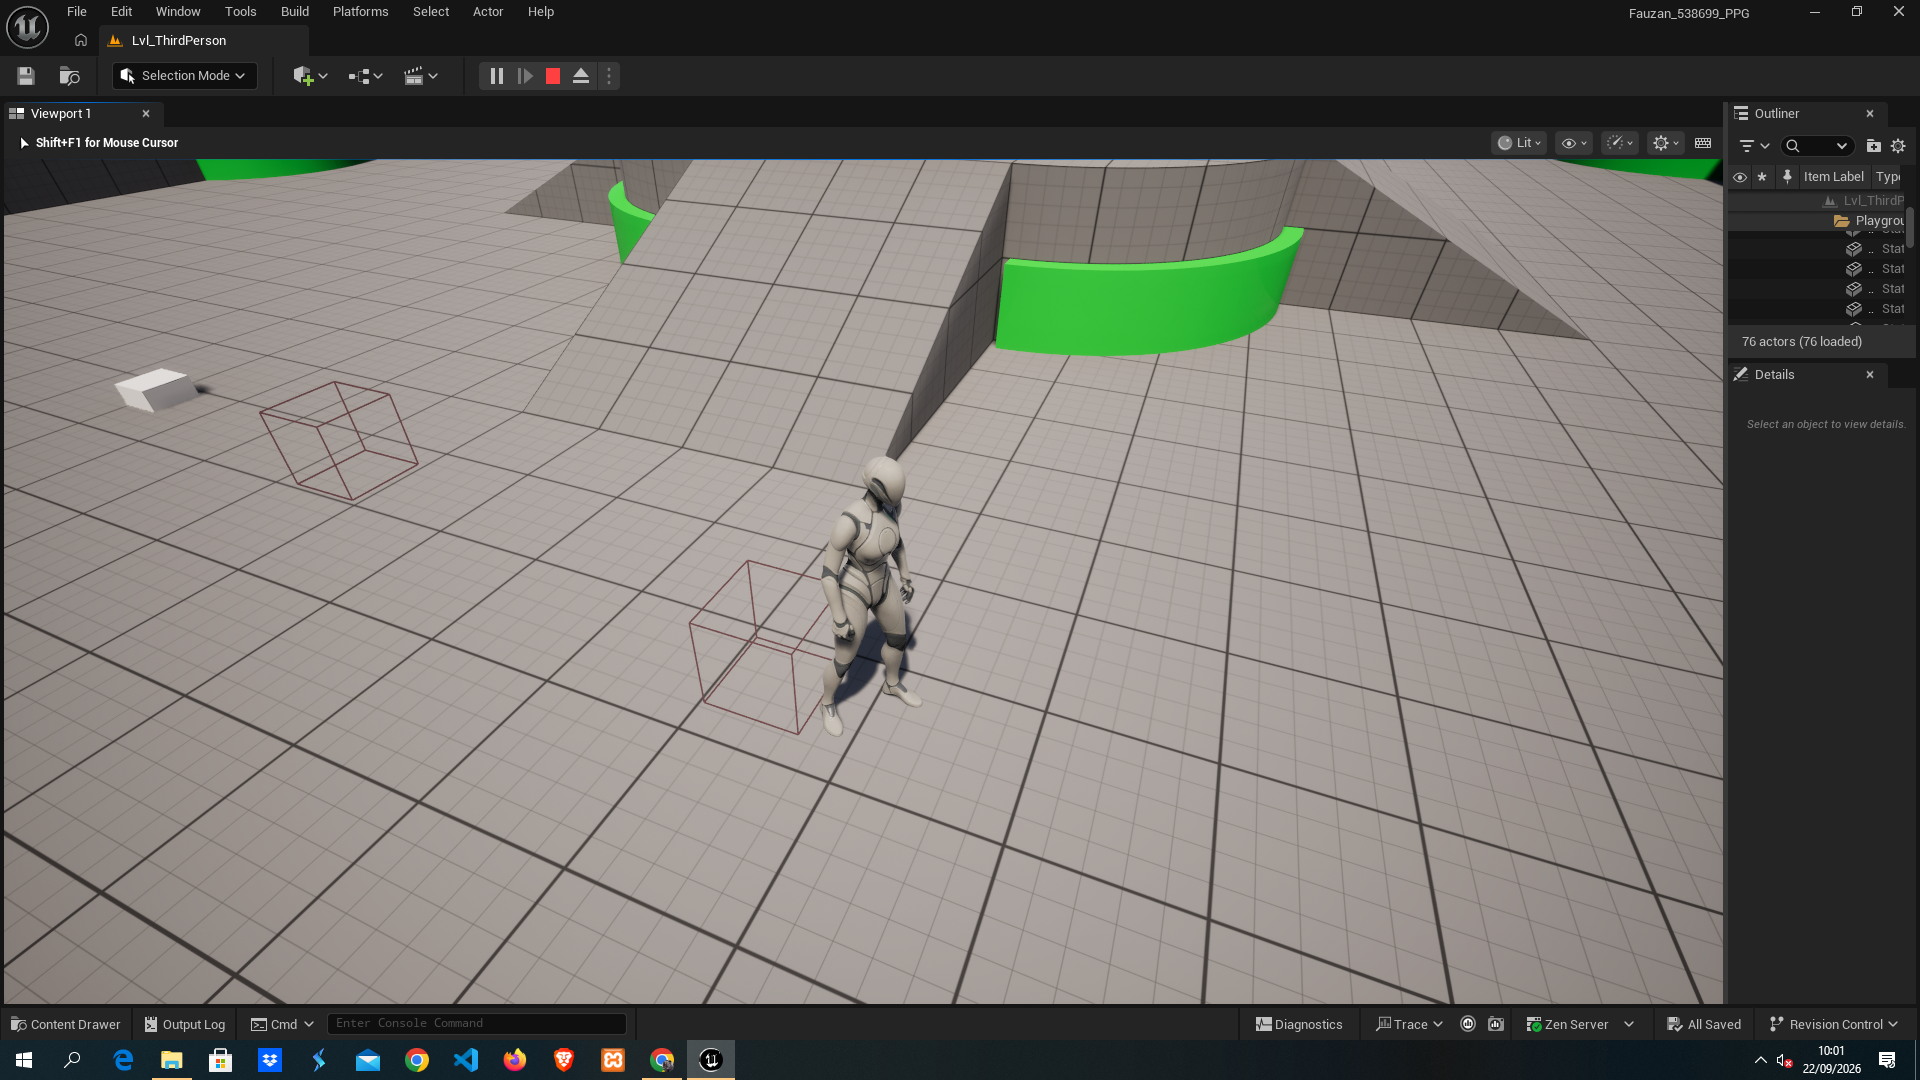
\includegraphics[width=0.8\textwidth]{resource/Dokumentasi/35.png}
  \caption{Penetapan Default Value Variabel Damage Sebesar 30.0}
  \label{fig:set-default-value-damage}
\end{figure}

\par Langkah berlanjut dengan menetapkan nilai bawaan variabel sebagaimana tampak pada Gambar \ref{fig:set-default-value-damage}. Setelah melakukan kompilasi pada \texttt{BP\_Collision}, saya mengisi angka 30.0 pada kolom \textit{Default Value} variabel \texttt{Damage} melalui panel \textit{Details}. Nilai 30.0 ini bertindak sebagai parameter kerusakan standar yang akan diterapkan secara otomatis kepada pemain setiap kali terjadi peristiwa overlap apabila desainer level tidak menentukan nilai khusus pada aktor tersebut.

\begin{figure}[H]
  \centering
  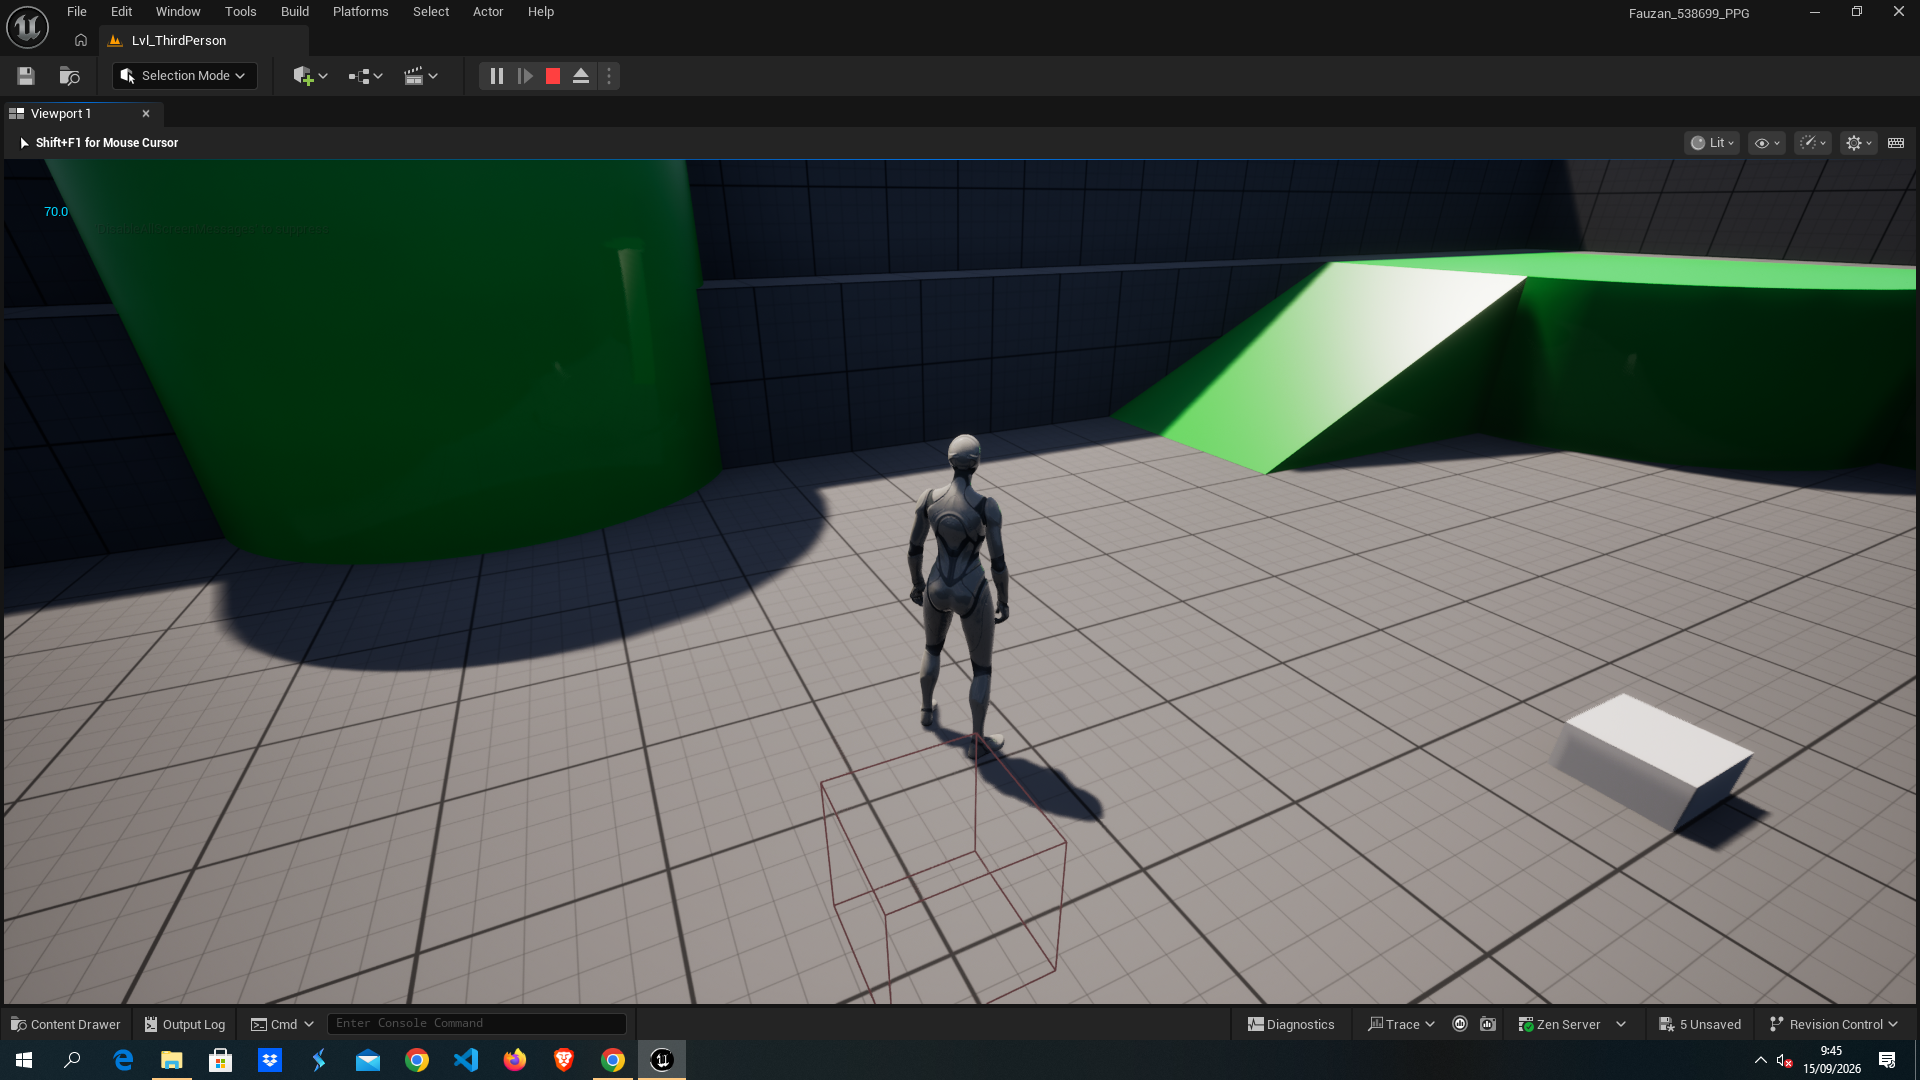
\includegraphics[width=0.8\textwidth]{resource/Dokumentasi/36.png}
  \caption{Menghubungkan Variabel Damage ke Node TakeDamage (Message)}
  \label{fig:connect-var-damage-to-message}
\end{figure}

\par Berdasarkan Gambar \ref{fig:connect-var-damage-to-message}, saya menyeret variabel \texttt{Damage} ke kanvas \textit{Event Graph} sebagai node \textit{getter}, kemudian menyambungkan pin keluarannya langsung menuju ke pin parameter masukan \texttt{AmountDamage} pada node fungsi antarmuka \texttt{TakeDamage (Message)}. Konfigurasi ini menyempurnakan alur logika visual di mana nilai kerusakan yang dikirimkan ke karakter pemain kini sepenuhnya bersumber dari variabel dinamis yang fleksibel.

\begin{figure}[H]
  \centering
  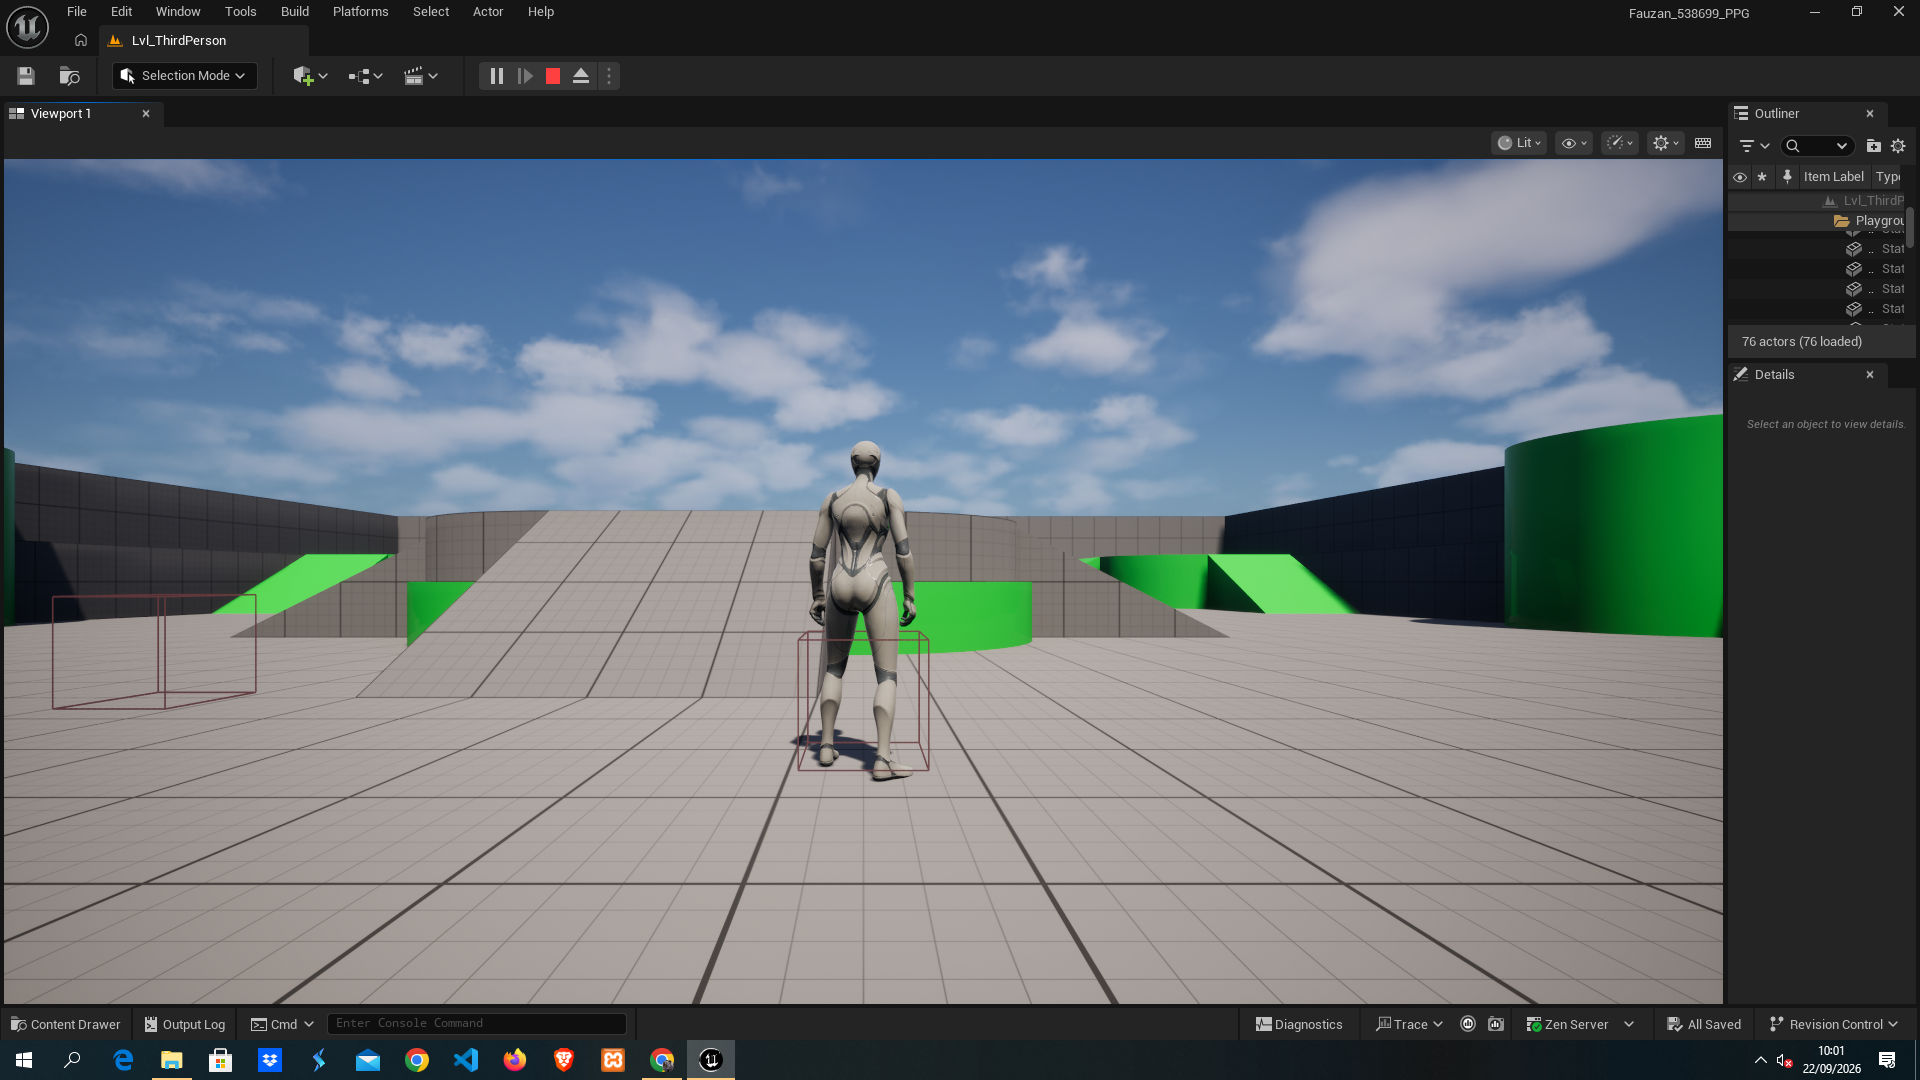
\includegraphics[width=0.8\textwidth]{resource/Dokumentasi/37.png}
  \caption{Konfigurasi Nilai Variabel Damage pada Panel Details di Level Editor}
  \label{fig:configure-damage-instance-details}
\end{figure}

\par Pada Gambar \ref{fig:configure-damage-instance-details}, saya kembali ke jendela utama level editor dan memilih aktor instansiasi \texttt{BP\_Collision} yang telah diletakkan di viewport arena permainan. Pada panel \textit{Details} di kategori \textit{Default}, variabel \texttt{Damage} kini berhasil muncul sebagai bidang masukan numerik yang dapat disunting langsung secara leluasa oleh desainer level tanpa perlu menyentuh grafik logika visual \textit{Blueprint} sama sekali.

\begin{figure}[H]
  \centering
  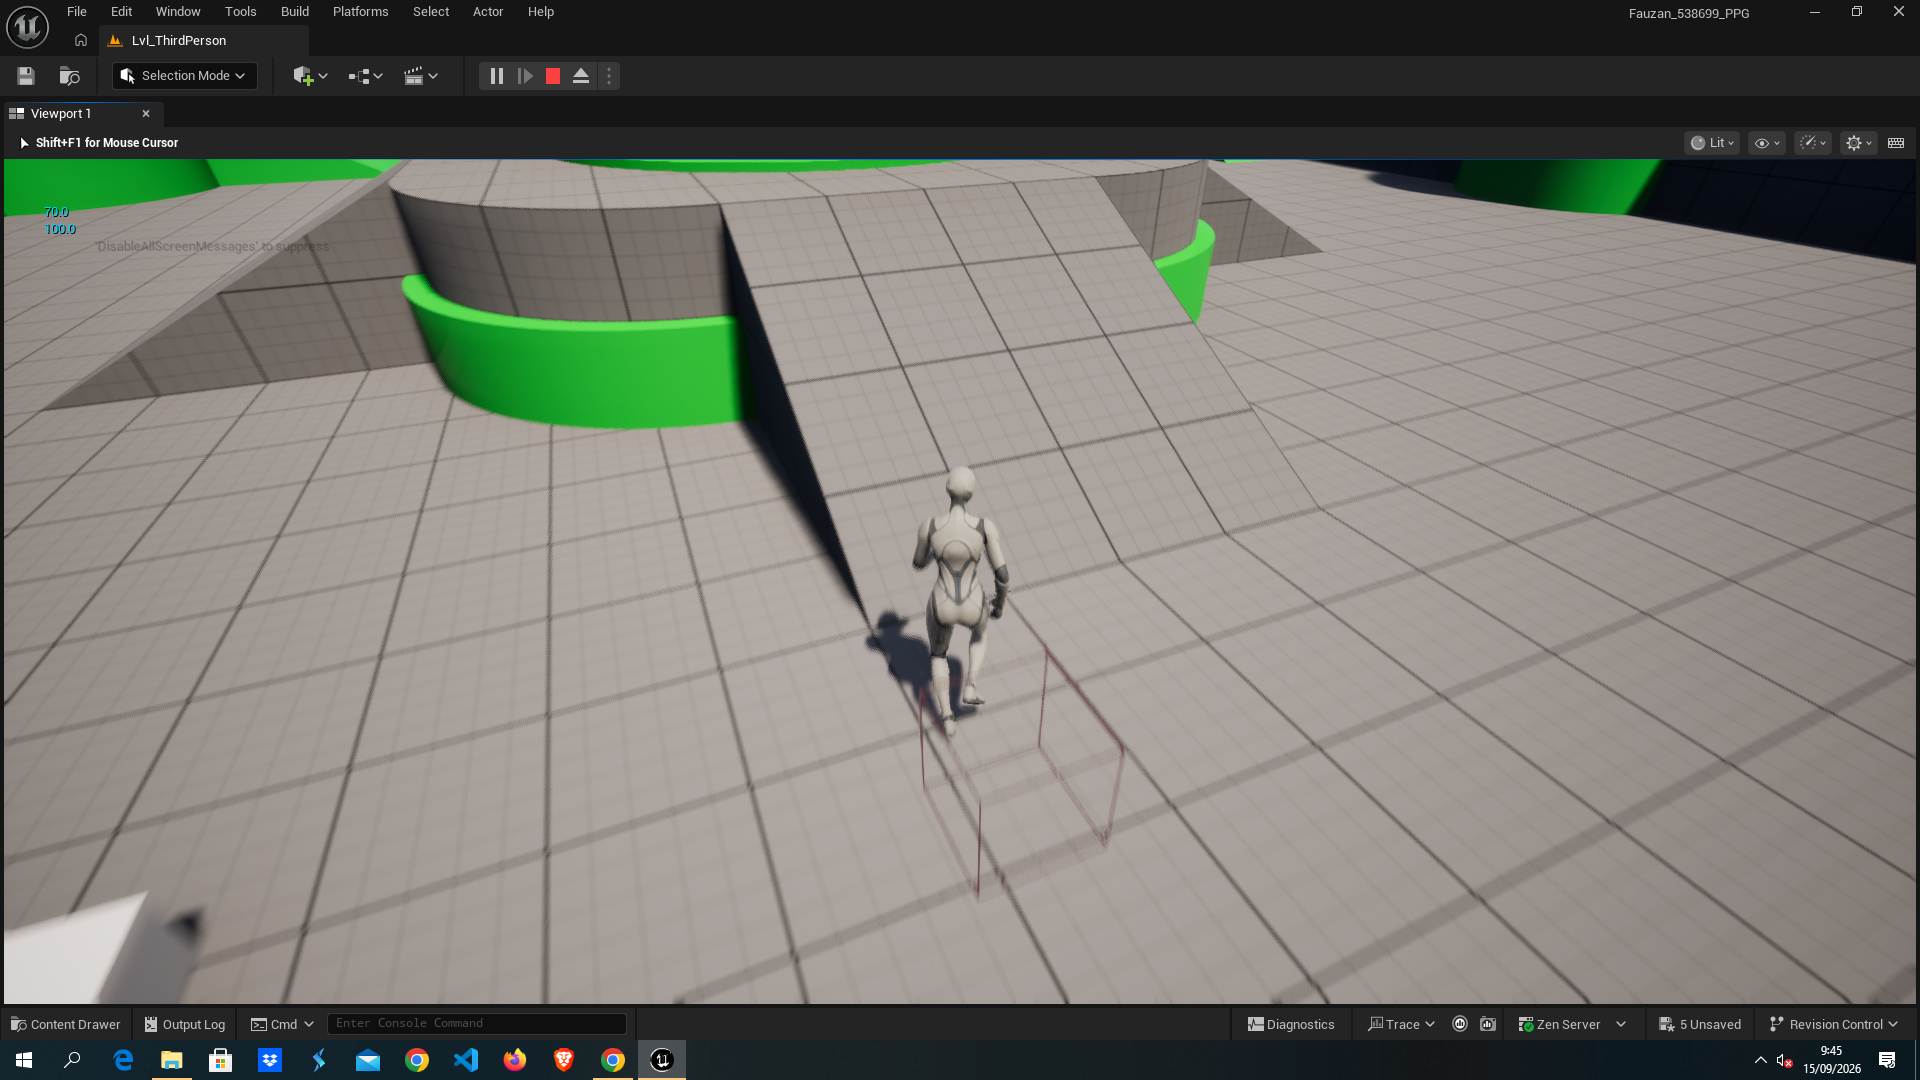
\includegraphics[width=0.8\textwidth]{resource/Dokumentasi/38.png}
  \caption{Pengujian Play-in-Editor dan Penurunan Kesehatan Karakter}
  \label{fig:pie-test-damage-overlap}
\end{figure}

\par Berdasarkan Gambar \ref{fig:pie-test-damage-overlap}, saya memulai pengujian simulasi interaktif menggunakan mode \textit{Play-in-Editor} (PIE) dengan menekan tombol pintasan \texttt{Alt + P}. Di dalam dunia permainan, volume kotak tabrakan \texttt{BP\_Collision} terlihat jelas berupa kerangka kawat kuning di lantai arena karena opsi \texttt{Hidden in Game} telah dimatikan sebelumnya. Saya menggerakkan karakter pemain memasuki area kotak tabrakan tersebut; seketika terjadi peristiwa overlap, sistem berhasil mengeksekusi pesan antarmuka \texttt{TakeDamage} dan memicu pengurangan nilai variabel \texttt{Health} karakter sebesar 30.0 secara bertahap dari 100 menjadi 70, kemudian 40, hingga menyentuh angka 10 saat karakter terus melintasi perangkap.

\begin{figure}[H]
  \centering
  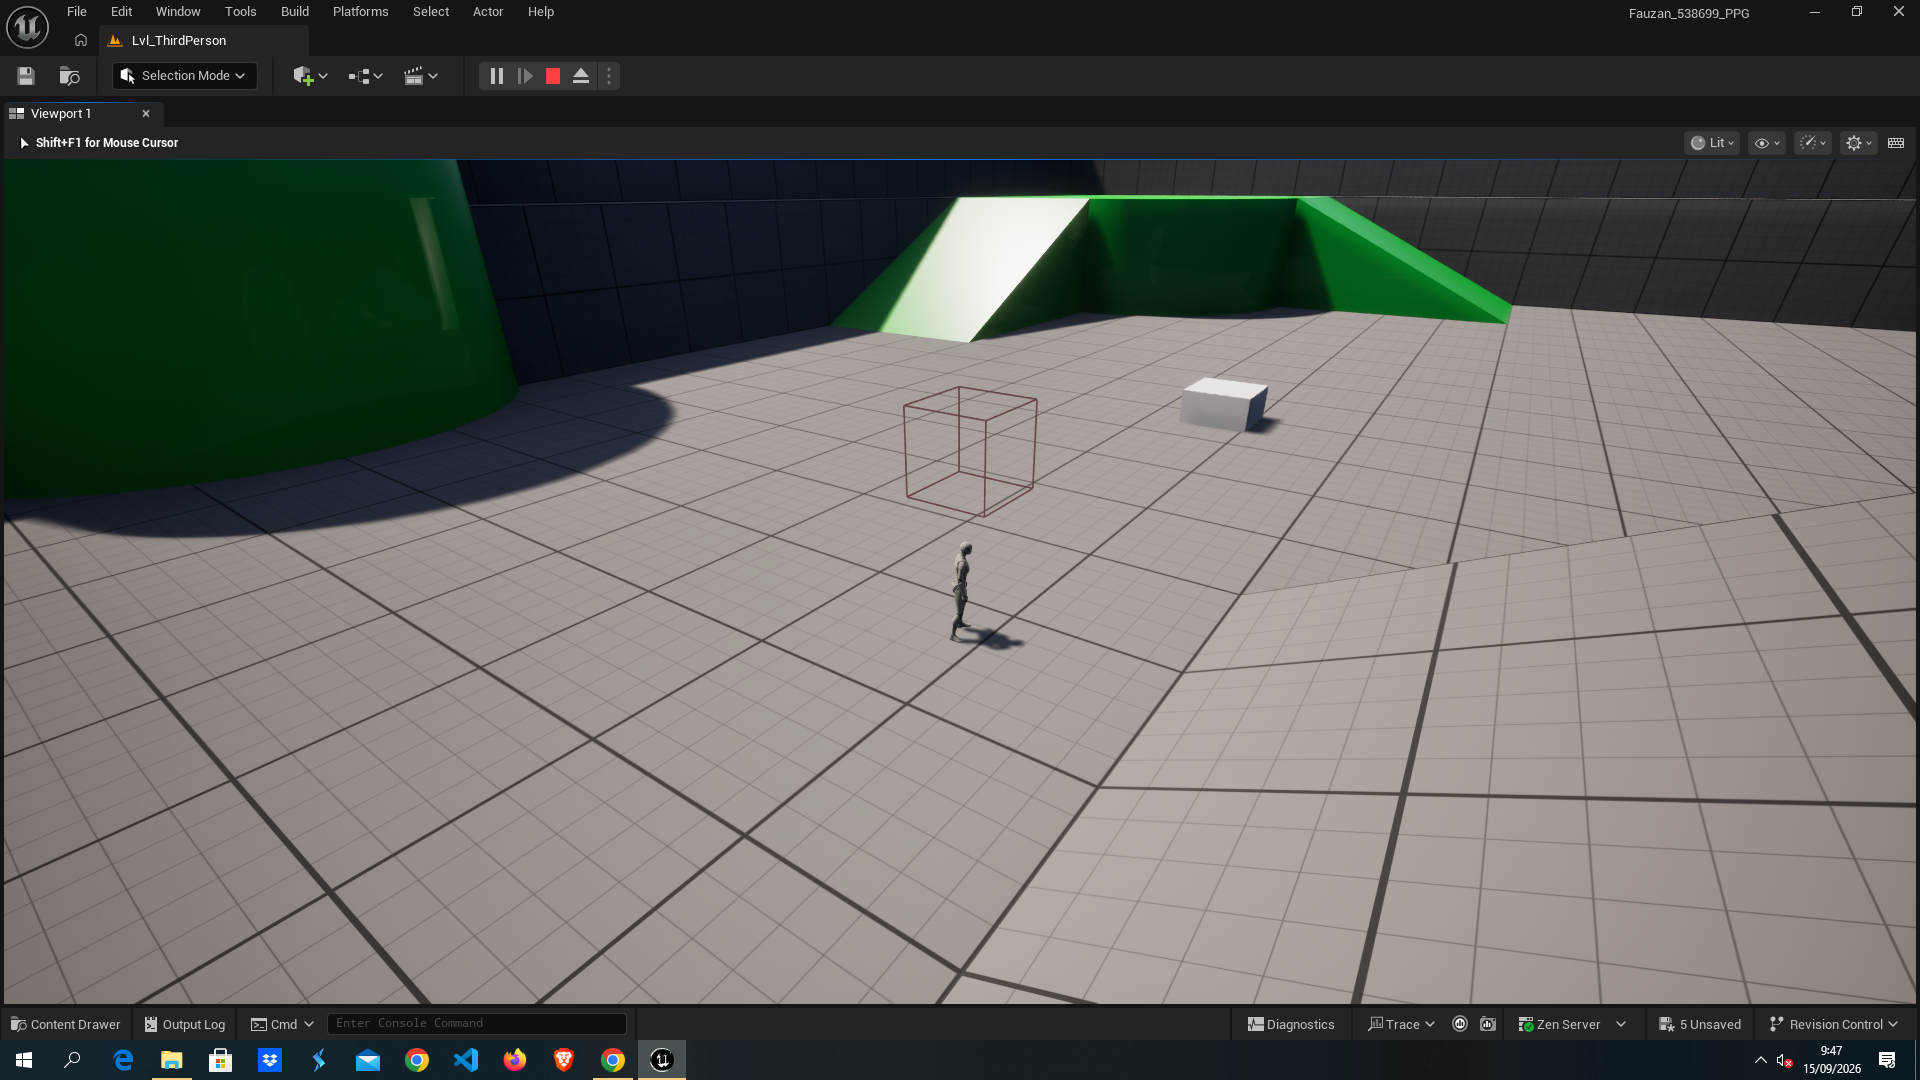
\includegraphics[width=0.8\textwidth]{resource/Dokumentasi/39.png}
  \caption{Validasi Pemicuan OnDeath dan Perubahan Skala Transformasi Karakter}
  \label{fig:pie-test-death-scale}
\end{figure}

\par Puncak pengujian divalidasi pada Gambar \ref{fig:pie-test-death-scale}, di mana saya menggerakkan karakter kembali melintasi kotak tabrakan hingga sisa nilai variabel \texttt{Health} mencapai batas minimum 0.0. Pada momen ini, fungsi \texttt{ModifyHealth} pada komponen \texttt{BPC\_Health} secara tepat mengevaluasi kondisi `Health <= 0.0` dan langsung memicu pemancaran sinyal \textit{Event Dispatcher} \texttt{OnDeath}. Karakter pemain (\texttt{BP\_ThirdPersonCharacter}) yang telah mengikat pendengar terhadap event tersebut secara responsif mengeksekusi node \texttt{Set Actor Scale 3D}, menyusutkan ukuran tubuh karakter menjadi skala 0.9 secara instan. Hasil pengamatan ini membuktikan secara konklusif bahwa seluruh rantai arsitektur sistem yang meliputi \textit{Actor Component}, \textit{Blueprint Interface}, dan \textit{Box Collision} telah terintegrasi secara utuh, harmonis, dan berfungsi sempurna sesuai rancangan teknis yang diharapkan.

\section{Hasil Akhir}

\par Berdasarkan serangkaian tahapan perancangan, implementasi, dan pengujian yang telah saya laksanakan pada Praktikum Pertemuan 4 ini, saya memperoleh sejumlah hasil akhir serta kesimpulan analitis teknis sebagai berikut:

\begin{enumerate}[label=\alph*.]
  \item \textbf{Arsitektur Logika Modular Berbasis Actor Component:}
        Saya berhasil merancang dan mengimplementasikan komponen logika kesehatan mandiri (\texttt{BPC\_Health}) yang memisahkan tanggung jawab pengelolaan atribut kesehatan dari kelas aktor utama. Dengan enkapsulasi logika penambahan, pengurangan, pembatasan nilai (\textit{clamping} antara 0.0 dan \texttt{MaxHealth}), serta evaluasi kondisi kematian, komponen ini dapat digunakan kembali secara fleksibel pada entitas aktor lain tanpa perlu menulis ulang logika yang sama.
        
  \item \textbf{Mekanisme Komunikasi Terkopel Rendah dengan Blueprint Interface:}
        Saya berhasil menerapkan komunikasi antar-Aktor melalui \textit{Blueprint Interface} \texttt{BPI\_Overlap} dengan fungsi \texttt{TakeDamage}. Metode ini meniadakan dependensi \textit{hard casting}, sehingga \texttt{BP\_Collision} dapat menyalurkan sinyal kerusakan ke aktor tujuan tanpa mengetahui kelas aslinya dan mencegah \textit{crash} bila target belum mengimplementasikan antarmuka tersebut.
        
  \item \textbf{Penerapan Paradigma Event-Driven dengan Event Dispatcher:}
        Saya berhasil memanfaatkan \textit{Event Dispatcher} \texttt{OnDeath} milik \texttt{BPC\_Health} yang diikat (\textit{bind}) oleh karakter pemain saat \textit{Event BeginPlay}. Komunikasi asinkron ini memungkinkan komponen kesehatan menyiarkan peristiwa penting ke aktor pemilik tanpa dependensi sirkular, di mana karakter langsung menyusutkan skala tubuhnya (\texttt{Set Actor Scale 3D} menjadi 0.9) saat batas kematian terpenuhi.
        
  \item \textbf{Integrasi Sistem Tabrakan Fisik Spasial:}
        Saya berhasil mengonfigurasi komponen \textit{Box Collision} pada aktor \texttt{BP\_Collision} untuk mendeteksi peristiwa perlintasan fisik (\textit{overlap}) secara akurat. Pengaturan visibilitas batas kawat dengan menonaktifkan properti \texttt{Hidden in Game} sangat membantu proses verifikasi dan \textit{debugging} di ruang tiga dimensi saat simulasi berlangsung.
        
  \item \textbf{Parameterisasi Dinamis melalui Instance Editable Variable:}
        Saya berhasil menerapkan parameterisasi nilai kerusakan pada aktor \texttt{BP\_Collision} menggunakan variabel bertipe \textit{Float} dengan opsi \textit{Instance Editable} aktif. Hal ini memberikan kemudahan bagi desainer level untuk memodifikasi parameter kerusakan per instansiasi objek secara langsung melalui panel \textit{Details} di editor level tanpa perlu menyentuh grafik logika \textit{Blueprint}.
        
  \item \textbf{Validasi Fungsional Menyeluruh melalui Play-in-Editor (PIE):}
        Melalui simulasi interaktif \textit{Play-in-Editor}, saya memvalidasi bahwa seluruh subsistem telah terintegrasi secara utuh dan bekerja sesuai alur spesifikasi teknis: karakter yang memasuki volume tabrakan secara konsisten mengalami pengurangan nilai kesehatan, terlindung dari anomali nilai negatif berkat mekanisme pembatasan matematis, dan berhasil mengeksekusi respons visual penyusutan ukuran tubuh ketika titik kesehatan mencapai angka nol.
\end{enumerate}

\end{document}